\documentclass[12pt,twoside]{book}

%encodage en XeLaTeX
\usepackage{fontspec}

\usepackage{imakeidx}
%\makeindex

%création hyperliens
\usepackage{hyperref}
\hypersetup{%
pdfauthor={Marion Charpier},
pdftitle={titre},
pdfsubject={sujet},
pdfkeywords={premier mot-clé} {deuxième mot-clé}
}

%charger les langues
\usepackage[english,french]{babel}
\usepackage{csquotes}

%\usepackage{glossaries}
%\makeglossaries

%mise en page
\usepackage[margin=2.5cm]{geometry}
\usepackage{setspace}%permet de définir l'interligne
\onehalfspacing % 1.5
\setlength\parindent{1cm} % indentation des paragraphes

\usepackage{lettrine}%pas obligatoire

%bibliographie
\usepackage[backend=biber,style=enc,maxbibnames=10,sorting=nyt]{biblatex}
\FrenchFootnotes
\AddThinSpaceBeforeFootnotes
\addbibresource{Mémoire_M2_TNAH_Charpier.bib}

%tous les paquets dont vous avez besoin : tableau, image, etc
\usepackage{url}
\usepackage{array}
\usepackage{booktabs}
\usepackage{graphicx}
\usepackage{amsmath}
\usepackage{makeidx}
\makeindex

\author{Marion Charpier}
\title{\textit{Computer vision} appliquée à l'analyse desources visuelles médiévales}
\date{Date}


\begin{document}

\begin{titlepage}

\begin{center}

    \bigskip

    \begin{large}
        ÉCOLE NATIONALE DES CHARTES\\
        UNIVERSITÉ PARIS, SCIENCES \& LETTRES
    \end{large}    


\begin{center}\rule{2cm}{0.02cm}\end{center}

\bigskip
\bigskip
\bigskip

\begin{Large}
    \textbf{Marion Charpier}
\end{Large}

%selon le cas

\begin{normalsize}
 \textit{licenciée ès lettres}\\
 \textit{diplômée de master}
\end{normalsize}

\bigskip
\bigskip
\bigskip

\begin{Huge}
\textbf{\textit{COMPUTER VISION} APPLIQUÉE À L'ANALYSE DE SOURCES VISUELLES MÉDIÉVALES}\\
\end{Huge}
\bigskip
\bigskip
\begin{Large}
    \textbf{EXPLORATION ET IMPLICATIONS HISTORIQUES}
\end{Large}

\vfill

\begin{large}
    Mémoire pour le diplôme de master\\
   \og Technologies numériques appliquées à l'histoire\fg{}\\
   \bigskip
   2023
\end{large}



\end{center}
\end{titlepage}


\frontmatter

\chapter{Résumé}

\medskip
Ce mémoire a été réalisé à la suite d’un stage de 4 mois au sein du laboratoire \textit{Digital History} de l’université Humboldt de Berlin. L'objectif principal de notre stage était d'explorer et d'appliquer divers outils technologiques de reconnaissance d'images pour analyser des données historiques, en se concentrant notamment sur les données héraldiques et les livres d'heures. Nous avons cherché à comprendre et à utiliser l'analyse sémantique des données, en mettant l'accent sur la détection de motifs iconographiques au sein des miniatures et en développant des modèles pour repérer les supports d'écriture. Notre démarche visait à intégrer la \textit{computer vision} dans le cadre d'une recherche historique portant sur des documents médiévaux. Les trois ensembles de données sur lesquels nous avons travaillé - à savoir les armoiries, les miniatures et les supports d'écriture - nous ont permis de saisir l'utilité de la \textit{computer vision }pour traiter de manière automatisée et à grande échelle des collections historiques, tout en nous confrontant aux défis inhérents à une telle approche.

Ce mémoire s’attache donc à décrire les différentes méthodologies déployées pour appliquer un traitement par \textit{computer vision} à des données iconographiques médiévales, en examinant en détail les différentes étapes cruciales afin d’assurer des résultats significatifs. Il rend également compte des résultats des différents modèles que nous avons formés. Ce faisant, nous présentons les différentes stratégies adoptées pour améliorer les détections et proposons des perspectives pour perfectionner la robustesse des modèles obtenus. 
.\\

\textbf{Mots-clés} : TNAH, \textit{Computer vision} ; \textit{Machine learning} ; Intelligence artifielle ; YOLO ; IIIF ; \textit{Digital History} ; Héraldique, Livres d'heures. \\

\textbf{Informations bibiographiques} : Marion Charpier, \textit{Computer Vision appliquée à l'analyse de sources visuelles médiévales. Exploration et implications historiques}, mémoire de master \og Technologies numériques appliquées à l'histoire\fg , dir. [Dominique Stutzmann, Torsten Hiltmann et Emmanuelle Bermès], École nationale des chartes, 2023.

\chapter{Remerciements}

\lettrine{J}e souhaite ici adresser mes remerciements à toutes les personnes qui m’ont permis de faire de cette année une belle aventure aussi bien intellectuelle qu’humaine. 

Je tiens à remercier Torsten Hiltmann pour m’avoir accueilli au sein du laboratoire \textit{Digital History }à Berlin. Je remercie également l’équipe du laboratoire, en particulier Sophie Eckenstaler et Philipp Schneider qui ont tous deux étés des aides précieuses pendant ce stage.

Je remercie chaleureusement Dominique Stutzmann pour avoir accepté de me suivre pendant ces quatre mois de stage. Sa bienveillance, sa patience et ses précieux conseils ont aiguillé ma réflexion et permis de progresser rapidement dans un domaine qui m’était, il y a quelques mois encore, inconnu.

Je tiens également à remercier Emmanuelle Bermès pour sa présence indéfectible tout au long de cette année, pour sa patience et son écoute constante.

Enfin, je souhaite remercier les copains qui m’ont accompagnée dans cette belle aventure chartiste Thomas, Aude et Giorgia. Vous êtes les meilleurs !




\chapter{Bibliographie}
\printbibliography

\chapter{Introduction}


\begin{quote}
L’historien de demain sera programmeur ou ne sera pas \footcite{le_roy_ladurie_fin_1968}.
\end{quote}.


Cette conclusion de l’article ‘La fin des érudits’ de l’historien Emmanuel Le Roy Ladurie, à la fin des années 60, témoigne de l’intérêt que revêtent les avancées technologiques et la volonté de les intégrer dans le cadre de la recherche historique. Le point premier mis en avant par l’auteur est la possibilité d’étudier de vastes corpus de documents dont le traitement manuel par un seul individu serait long, fastidieux, voire irréalisable. L’objectif affiché de ce traitement massif des données est bien de les rendre reproductibles et accessibles au plus grand nombre. Si Emmanuel Le Roy Ladurie évoque les cartes perforées bien loin de nos technologies contemporaines, il n’en reste pas moins que ces dernières décennies ont produit un nombre toujours croissant de données numériques librement accessibles. \\

L’abondance des données disponibles constitue un terrain de jeu presque sans limite pour les historiens, ouvrant le champ à de nouvelles réflexions historiques, notamment dans le domaine de l'analyse et de la reconnaissance automatique des images. Le traitement computationnel des données historiques est favorisé par l'évolution des méthodes d'apprentissage automatique, en particulier la vision par ordinateur – ou \textit{computer vision}.  Ce domaine de l’intelligence artificiel repose sur des techniques de traitement d'images, d'apprentissage automatique (\textit{machine learning}) et plus spécifiquement d'apprentissage profond (\textit{deep learning}) et permet le développement d'algorithmes et de modèles capables d'analyser et d'interpréter des données visuelles, comme des images et des vidéos, pour en extraire des informations significatives. La \textit{computer vision} permet ainsi la formation de modèles capables de faire des prédictions et classifications sur des jeux de données étendus \footcite{pedersoli_elastic_2015}. 

\newpage
L'adoption croissante du cadre international d'interopérabilité des images (IIIF) par les institutions patrimoniales est un catalyseur technologique pour le développement de projets de recherche sur les sources historiques s’appuyant sur la \textit{computer vision.} En 2019, un milliard d'images étaient disponibles, dont environ 300 millions pour la période médiévale \footcite[p.2]{aouinti_illumination_2022}. Les premières expériences d'utilisation de la \textit{computer vision} appliquée aux données historiques et du protocole IIIF sont apparues dès 2017. La première édition de la compétition internationale sur l’analyse d'ouvrages anciens « Historical Book Analysis » a fourni un protocole d'évaluation pour traiter des problèmes spécifiques liés aux méthodes d’analyse d’images de documents anciens \footcite{mehri_hba_2017}. Dans ce cadre, la Bibliothèque nationale de France a conçu un jeu de données HBA dédié à l'analyse de la structure de la mise en page d'ouvrages anciens \footcite{noauthor_hba_2017}. En 2019, les travaux menés autour de l’outil ‘dhSegment’’ ont proposé une approche générique afin de segmenter des régions et d'extraire le contenu de différents types de documents historiques \footcite{oliveira_dhsegment_2018}. La même année, Jean-Philippe Moreux a lancé une étude visant à identifier et extraire l’iconographie des images et imprimés de la bibliothèque numérique Gallica, afin d’harmoniser et d’enrichir les métadonnées descriptives de ces images grâce à la \textit{computer vison} \footcite{moreux_recherche_2019}. L'année suivante, T. Monnier et M. Aubry ont présenté ‘docExtractor’, un outil générique pour l'extraction d'éléments visuels (lignes de texte, illustrations) à partir de documents historiques sans nécessité d'annotation de données réelles \footcite{monnier_docextractor_2020}.

\newpage
Les possibilités de recherche qu’offrent ces approches computationnelles pour l’analyse des données historiques numérisées ont rapidement intéressé les historiens et historiens de l’art \footcite{ufer_large-scale_2021}, en particulier les médiévistes, premiers à s’emparer des technologies nouvelles pour les adapter la recherche \footcite{unsworth_medievalists_2012}. En témoigne les nombreux projets consacrés à la segmentation, l’extraction et l’analyse iconographiques des manuscrits médiévaux. En 2009, Costantino Grana, Daniele Borghesani et Rita Cucchiara ont travaillé à la conception d’un modèle centré sur la segmentation automatique des manuscrits numérisés afin d'en extraire les éléments graphiques, puis d'en identifier les images significatives \footcite{grana_picture_2009}. Les études consacrées à l’analyse de la structure des manuscrits se sont également multipliées. La difficulté et l’intérêt du traitement automatisé des manuscrits médiévaux tient à leur nature complexe \footcite{yang_automatic_2017}. L’utilisation des protocoles IIIF a facilité l’accès et l’analyse de ces manuscrits, notamment l’extraction des enluminures des manuscrits numérisés \footcite{aouinti_illumination_2022}. \\

A ces approches d’analyse globale des manuscrits, des projets plus spécifiques dédiés à l’iconographie se sont développés en parallèle. Les objectifs de ces projets ne reposaient non pas sur la seule extraction de données, mais sur la qualification des objets spécifiques au sein de cycles iconographiques plus larges. Le travail proposé par Schlecht, Carqué, et Ommer s’intéresse à l'interaction et la communication entre les personnes représentées dans les manuscrits, en s’appuyant sur des postures caractéristiques des bras, des mains ou même d'un seul doigt. Les gestes jouent un rôle particulièrement important pour les chercheurs en communication symbolique dans la culture juridique médiévale. Le but est d’automatiser une analyse comparative des gestes légaux utilisés dans les manuscrits médiévaux \footcite{schlecht_detecting_2011}. 
Les analyses concluantes ont permis aux auteurs de poursuivre leurs recherches plus largement sur la communication non verbale dans les manuscrits illustrés \enlargethispage{\baselineskip} \footcite{bell_nonverbal_2013}. L’amélioration constante des modèles a permis la mise en place de projet plus complexes sur la représentation du chant et des groupes de chant représentés dans les manuscrits enluminés et accessible via le protocole IIIF \footcite{ibrahim_few-shot_2022}. Enfin, le projet VHS, débuté en 2020, a pour vocation d’étudier la circulation des connaissances scientifiques en s’appuyant sur l’analyse par computer vision de l'évolution et de la transformation des images dans les corpus scientifiques illustrés du Moyen Âge et de l'époque moderne \footcite{noauthor_computer_nodate}. \\

Ainsi, la pluralité et la diversité des études des sources iconographiques médiévales témoignent de la richesse de ce patrimoine et les projets consacrés à des tâches plus spécifiques sont nombreux. Le projet de recherche \textit{Digital Heraldry}, porté par Torsten Hiltmann et le laboratoire \textit{Digital Hitsory} de l’université Humboldt de Berlin, s’inscrit dans cette démarche. Ce projet s’appuie sur les méthodes de traitement informatique des données pour améliorer la recherche en héraldique, domaine crucial pour la compréhension des cultures et des sociétés occidentales du Moyen Âge au début des temps modernes \footnote{\url{https://digitalheraldry.org/}}. En effet, les armoiries constituent un des plus importants supports visuels de ces époques, pouvant indiquer une domination territoriale, le rang social ou l’identité de la famille, apparaissant aussi bien dans les manuscrits médiévaux que sur les peintures murales, les sculptures, les vitraux et les sceaux. Malgré leur importance en tant que symboles visuels, les armoiries ont souvent été négligées, voire ignorées dans leur pertinence par la recherche historiographique. Cela s’explique à la fois par la quantité d’armoiries existantes, la pluralité des supports sur lesquels elles se déploient et la diversité de leurs contextes d'utilisation. Le projet \textit{Digital Heraldry} vise à combler ces lacunes en utilisant l'apprentissage automatique et le Web sémantique pour collecter et analyser des données historiques numérisées, facilitant ainsi la description et l'identification semi-automatiques des armoiries. 

Dans ce cadre, nous avons entraîné de nouveaux modèles de détection des armoiries. Afin d'apprécier la robustesse de ces nouveaux modèles, nous avons automatisé les processus d’évaluation en nous appuyant sur les métriques propres à la computer vision. 

\newpage
En parallèle de cette mission, nous avons également entraîné différents modèles d'intelligence artificielle à segmenter l'information visuelle sur des ressources numérisées, en nous intéressant en particulier à la détection de miniatures sur des livres d'heures médiévaux. Nous nous sommes pour cela appuyés sur la base des informations disponibles dans le cadre du projet de recherche HORAE. Ce projet, initié en 2018 et achevé en 2020, vise à analyser les pratiques religieuses du Moyen Âge tardif en combinant, à travers les livres d’heures, l’intelligence artificielle appliquée à l’analyse d’image par ordinateur et le traitement automatique des langues (TALN) \footnote{\url{https://www.irht.cnrs.fr/fr/recherche/les-programmes-de-recherche/horae}}. Malgré leur importance, les livres d'heures ont été insuffisamment étudiés jusqu'à présent en raison de leur grand nombre, de leur complexité et de la répétitivité de leurs textes. Les livres d'heures représentent un ensemble vital et étendu pour appréhender la mentalité médiévale \footcite{stutzmann_texte_2021}. L'analyse des illustrations, en particulier des miniatures, est une composante complémentaire de ce projet centré sur le texte. Ces représentations visuelles révèlent les valeurs, les connaissances et les croyances du copiste, offrant un intérêt majeur pour les historiens. La complexité de leur analyse par intelligence artificielle à grande échelle réside dans la nature même de ces illustrations dont l’ordre et le contenu présentent une grande variabilité d’un manuscrit à l’autre. Par ailleurs, la dispersion de ces manuscrits dans de nombreuses bibliothèques mondiales a longtemps entravé toute analyse automatisée à grande échelle, jusqu'à l'introduction du cadre IIIF. \\

 Ainsi, l’objectif principal de notre stage était de s’emparer des différents outils technologiques de reconnaissance d’images pour les appliquer à des données historiques, en particulier les données héraldiques et les livres d’heures. Nous nous sommes également intéressés à l'analyse sémantique des données, en nous focalisant sur la détection de motifs iconographiques au sein des miniatures et en nous attachant à entraîner des modèles capables de détecter les différents supports d’écritures. Ce faisant nous nous sommes intéressés à l’utilisation de la \textit{computer vision} dans le cadre d’une recherche historique sur des matériaux médiévaux. Les trois ensembles de données sur lesquels nous avons travaillé – armoiries, miniatures et supports d’écritures – nous ont permis d’appréhender l’intérêt de la \textit{computer vision} pour traiter automatiquement à grande échelle des collections historiques mais aussi les problématiques qui peuvent être liées à une telle approche.
 
\newpage
 Nous présentons donc ici les modalités de mise en place d’un traitement par \textit{computer vision} de données iconographiques médiévales en détaillant les différentes étapes et le rôle clé qu’elles jouent afin de garantir des résultats pertinents. Nous présenterons ensuite les résultats des modèles entraînés ainsi que les différentes stratégies à mettre en place pour améliorer les détections en fonction des objectifs de recherche. 

\mainmatter

%utiliser des \input pour chaque partie par exemple

\part{Mise en place d'un traitement de données historiques par \textit{computer vision} : principes et modélisation}

\chapter{Introduction}
Nous verrons dans cette première partie comment mettre en place un projet de \textit{computer vision} appliqué à l’étude de sources iconographiques médiévales. Il nous importera d'explorer les différents algorithmes de définir les stratégies à appliquer pour la collecte des données et la constitution des \textit{datasets} d’entraînement et d’inférence. Nous nous attacherons également à expliciter les problématiques de modélisation d’une telle approche avant de nous intéresser aux différents modèles de \textit{machine learning} exploitables en fonction des besoins de la recherche.\\

Ainsi, nous présenterons dans les chapitres suivants les différentes étapes et approches à mettre en place pour concevoir le traitement des données, la mise en place des ontologies et les modalités d’entraînement des différents modèles, en utilisant des exemples concrets issus de l’expérience acquise durant notre stage.

\chapter{Modélisation : modèles et ontologie}

\section[Le choix des modèles ]{Le choix des modèles : Approche supervisée ou non supervisée }

Le \textit{machine learning} consiste à former des modèles, grâce à l’analyse d’un jeu de données, capables de faire des prédictions utiles sur de nouvelles données. La formation des modèles passe nécessairement par une phase d’apprentissage, dite aussi d’entraînement, qui repose principalement sur deux méthodes : l'apprentissage supervisé et l'apprentissage non supervisé.

\subsection{Modèle non supervisé}

Dans l'apprentissage non supervisé, il n'y a pas de superviseur, c’est-à-dire que les données d’entraînement ne sont pas étiquetées – ou annotées. Le modèle cherche alors à trouver des régularités dans les données d'entrée et mettre en lumière des correspondances et similarités cachées dans les données. L’intervention humaine n’est pas n’est pas nécessaire dans ce processus, à l’origine de la qualification de modèle « non supervisé ». \\

Avec un algorithme d'apprentissage non supervisé, l'objectif est d'obtenir des informations à partir d’un grand volume de données, de sorte que le modèle détermine lui-même ce qui est différent ou intéressant dans l'ensemble des données. L'utilisation la plus courante de l'apprentissage automatique non supervisé consiste à assembler les données en groupes d'exemples similaires pour découvrir la structure inhérente au corpus d’entraînement. Cette technique d’apprentissage appelée \textit{clustering}, implique la partition d'un certain ensemble de données en groupes dont les composantes se ressemblent selon une mesure de similarité \footcite{alpaydin_introduction_2014}. Un cas d’application sur des données iconographiques a été produit dans le cadre du projet VHS, où un algorithme non supervisé a été entraîné sur des manuscrits médiévaux de sorte à pouvoir identifier d’une part les différentes espèces animalières présentes dans le \textit{Physiologus} grec, d’autres par les différentes essences de plantes représentées dans le \textit{De Materica Medica} de Dioscorides \footcite{kaoua_image_2021}. \\

L’apprentissage non supervisé, nécessite l’utilisation d'outils puissants et complexes pour travailler avec de grandes quantités de données non classifiées. Par ailleurs, les méthodes d'apprentissage non supervisé peuvent produire des résultats extrêmement imprécis, nécessitant finalement une intervention humaine pour affiner et valider les variables de sortie.

\subsection{Modèle supervisé}

L'apprentissage supervisé est une approche d'apprentissage automatique qui se définit par l'utilisation d’ensemble de données annotées. Ces corpus sont conçus pour former des algorithmes capables de classer les données ou de prédire des annotations avec précision. L’intervention humaine précède et détermine l’entraînement, qui est de fait « supervisé ». \\

Dans l'apprentissage supervisé, l'algorithme « apprend » à partir d’un ensemble de données étiquetées, en faisant sur elles des prédictions itératives et en s'ajustant pour obtenir des résultats conformes aux données d’entraînement. Le modèle peut ainsi mesurer sa précision et s’améliorer à chaque itération. Si les modèles d'apprentissage supervisé tendent à être plus précis que les modèles d'apprentissage non supervisé, ils nécessitent une intervention humaine initiale pour étiqueter les données de manière appropriée. L’intérêt d’une telle approche en recherche historique est que l’on peut concevoir une problématique précise et attendre des résultats pertinents pour y répondre. Dans le cas d’une recherche sur les spécificités iconographiques des différentes espèces de serpents présentes dans les bestiaires médiévaux, il serait nécessaire d’annoter chaque serpent de sorte que le modèle soit capable de détecter correctement les différentes espèces dans des données nouvelles. Les enjeux de l’exploration sont connus à l’avance. 

\subsection{Quel modèle utiliser ?}

La principale différence entre ces deux approches réside dans le fait que les modèles supervisés sont entraînés pour apprendre à prédire des résultats spécifiques en se basant sur des exemples connus, tandis que les modèles non supervisés recherchent des structures, des modèles ou des relations cachées sans avoir de résultats de référence prédéfinis. \\

Le choix de l’une ou l’autre approche se détermine en fonction de la problématique historique et des données utilisées. Dans le cadre des différents projets sur lesquels nous avons travaillé au sein du laboratoire \textit{Digital History}, l’approche supervisée a été privilégiée. Dans le cadre du projet \textit{Digital Heraldry}, l’utilisation de la \textit{computer vision} vise à identifier et classer les éléments et motifs héraldiques, ainsi que les formes sur lesquels ils se déploient. Dans le cadre des projets \textit{Miniatures} et \textit{Books in Books}, il s’agit également de détecter des objets précisément identifiés et non de rechercher des structures sous-jacentes. Ainsi, le choix s'est naturellement porté sur des modèles supervisés.\\ 

La classification des données volumineuses peut être un véritable défi pour l'apprentissage supervisé, mais les modèles produits sont plus précis et fiables. L'apprentissage non supervisé peut quant à lui traiter de grands volumes de données en temps réel, mais engendre un manque de transparence dans la façon dont les données sont regroupées et un risque plus élevé de résultats inexacts.

\section[Architecture supervisée]{Architecture supervisée}


\subsection{Modèles à deux temps (Two-stage detection)}

Les modèles à deux temps, tels que R-CNN (\textit{Region-based Convolutional Neural Network}) et ses variantes, proposent une approche en deux étapes distinctes pour identifier et localiser les objets d'intérêt dans une image. Cette approche, comme celle à un temps, repose sur une classe de réseaux de neurones profonds, dit réseaux de neurones convolutifs -- \textit{Convolutif Neuronal Network} -- spécialement conçus pour traiter des données structurées en grille, ou matrices, telles que des images et des vidéos. Un réseau neuronal convolutif typique se compose d'une combinaison des couches suivantes :

\newpage

\begin{itemize}
    \item Couche convolutive (\textit{convolutional layers}) : Couche d'un réseau neuronal profond dans laquelle un filtre convolutif passe le long d'une matrice d'entrée. La convolution consiste à appliquer un filtre à une petite région de l'image, puis à déplacer le filtre sur toute l'image pour créer une carte de caractéristiques.
    \item Couche de \textit{pooling} (\textit{pooling layers}) : Réduction d'une matrice (ou de matrices) créée(s) par une couche convolutive antérieure en une matrice plus petite. Cela réduit le nombre de paramètres du modèle tout en préservant les caractéristiques importantes.
    \item Couche dense (\textit{fully connected layer)} : Une couche cachée dans laquelle chaque nœud est connecté à chacun des nœuds de la couche cachée suivante \footnote{\url{https://developers.google.com/machine-learning/glossary?hl=fr\#convolutional_neural_network}}
\end{itemize}

\paragraph{}Les CNN sont composés de plusieurs couches de convolution et de \textit{pooling} empilées les unes sur les autres. Plus le réseau est profond, plus il est capable d'apprendre des caractéristiques abstraites et complexes. \\

La détection d'objets en deux temps utilise donc deux passages de l'image d'entrée pour prédire la présence et l'emplacement des objets. Le premier passage est utilisé pour générer un ensemble de propositions ou d'emplacements potentiels d'objets. Ces propositions sont indépendantes de la catégorie, ce qui signifie qu'elles ne sont pas encore associées à des types d'objets spécifiques. Le second passage est utilisé pour affiner ces propositions et faire des prédictions finales. Les régions d'intérêt générées précédemment sont soumises à des CNN qui classifient chaque région d'intérêt en prédéfinissant à quelle classe d'objet elle appartient (par exemple boa ou aspic), puis ajuste la position et la forme de la boîte englobante autour de l'objet détecté grâce aux couches denses. Cela permet d'obtenir des détections plus précises en ajustant les boîtes de délimitation autour des objets \footcite[p. 2-3]{jiao_survey_2019}. \\

Les modèles en deux temps permettent une analyse plus fine des régions d'intérêt, ce qui peut conduire à des prédictions plus précises. En revanche, cette approche nécessite deux passages pour chacune des images à analyser, ce qui en fait un modèle plus coûteux en termes de calcul. 

\newpage

\subsection{Modèles à un temps (One-Stage detection)}

Les modèles à un temps, tels que YOLO (\textit{You Only Look Once}) et SSD (\textit{Single Shot MultiBox Detector}), effectuent la détection d'objets en un seul passage de l’image. Ils prédéfinissent un ensemble de boîtes englobantes à différentes échelles et positions dans l'image, puis utilisent des réseaux neuronaux convolutifs pour prédire les probabilités de classe et les ajustements de localisation pour chaque boîte englobante. Cela signifie que la détection et la classification sont effectuées simultanément pour chaque région prédéfinie. \\

L’intérêt essentiel de cette approche est que le modèle peut traiter l'ensemble de l'image en un seul passage, détection et localisation, permettant d’accroître la vitesse de traitement des images. Ces algorithmes peuvent être utilisés pour détecter des objets en temps réel dans des environnements où les ressources sont limitées. En revanche, la précision de détection, notamment sur des petits objets ou des chevauchements de nombreux objets, sera beaucoup moins performante. \\

La principale différence entre ces deux approches réside dans le compromis entre vitesse et précision. Les modèles à un temps sont généralement plus rapides car ils effectuent la détection en un seul passage, mais ils peuvent être moins précis dans la localisation fine des objets. Les modèles à deux temps, en revanche, sont plus précis dans la localisation car ils effectuent des étapes séparées pour générer des propositions de régions et pour effectuer la détection finale, mais ils sont généralement plus lents en raison de ces étapes distinctes.



\subsection{YOLO}

\textit{You Only Look Once} (YOLO), comme son nom l’indique, est un modèle de détection d'objets à un temps. YOLO propose d'utiliser un réseau neuronal entièrement convolutif (CNN) de bout en bout afin de prédire les boîtes englobantes (\textit{bounding box}) et les probabilités de classe en une seule fois. Cette approche diffère de celle adoptée par les algorithmes de détection d'objets précédents qui réutilisaient des classificateurs pour effectuer la détection \footcite{redmon_you_2015}. \\

L'architecture spécifique du modèle CNN pour YOLO est plus précise que les autres modèles à un temps. YOLO divise une image d'entrée en une grille de taille S x S. Si le centre d'un objet tombe dans une cellule de la grille, cette cellule est responsable de la détection de cet objet. Chaque cellule de la grille prédit des boîtes de délimitation et des scores de confiance pour ces boîtes. Ces scores de confiance reflètent le degré de confiance du modèle dans la présence d'un objet dans la boîte et le degré de précision de la boîte prédite.\\

Plusieurs boîtes englobantes sont prédites par cellule de la grille. Lors de l'apprentissage, il est important que chaque objet soit attribué à un seul prédicteur de boîtes pour que la prédiction soit la plus précise possible. Lorsqu'un objet est détecté, YOLO attribue la prédiction de la boîte englobante à un prédicteur spécifique en fonction de la proximité du centre prédit de la boîte englobante par rapport au centre réel de l'objet (coordonnées du centre de la vérité terrain). Cela signifie que le prédicteur dont la prédiction de centre est la plus proche du centre réel de l'objet est désigné comme « responsable » de la prédiction de cet objet. En attribuant la prédiction d'une boîte englobante en fonction de la proximité du centre, YOLO s'assure que chaque objet est associé à un seul prédicteur pour une détection précise. Cette approche favorise la spécialisation des prédicteurs, ce qui signifie que chaque prédicteur devient plus compétent pour prédire des objets de certaines tailles, formes ou catégories, ce qui permet d’accroître les performances globales du modèle en termes de détection d’objets. \\

Depuis le lancement de YOLO en 2015, de nombreuses versions toujours plus performantes se sont succédées. L’équipe du laboratoire \textit{Digital History} utilisait jusqu’à notre arrivée la version 4, notre but était d’entraîner de nouveaux modèles avec YOLOv7 plus performant, plus précis et rapide que la version 4 \footcite{redmon_you_2015}. Cependant, le déploiement de YOLOv8, encore plus performant que YOLOv7 et utilisable avec Python, a convaincu le laboratoire de l’utiliser en priorité \footcite{yolov8_ultralytics}. Les modèles entraînés avec YOLOv4 ont dû être délaissés en raison de l’incompatibilité entre les différentes architectures de YOLO, conçues pour améliorer les performances et la précision. Ces changements architecturaux rendent difficile la compatibilité entre les versions. \\

\paragraph{Conclusion}Ainsi, le choix des modèles et des architectures doit être défini en fonction des besoins de la recherche et de la problématique dans laquelle le traitement des données par \textit{computer vision} se déploie. Le cadre mis en place par le laboratoire \textit{Digital History} est l’utilisation d’un modèle supervisé à un temps, l’algorithme YOLOv8 a été privilégié en raison de ces performances en termes de puissance et de rapidité.

\newpage
\section{Ontologie et structuration des données}

Le principe de l’ontologie, selon Gruber, est une spécification explicite d'une conceptualisation, c’est-à-dire une représentation simplifiée et compréhensible d'un concept pensée dans un but spécifique \footcite{gruber_translation_1993}. L’ontologie contient donc les objets, les concepts et les autres entités qui sont supposés exister dans un certain domaine d'intérêt et les relations qui existent entre eux. La construction de l’ontologie permet de définir un cadre conceptuel applicable à divers scénarios et peut être utilisée comme guide de référence lors de la production de données lisibles. 

\subsection{Les principes de l’ontologie en \textit{machine learning}}

Dans le cadre d’un travail de \textit{computer vision} avec modèle supervisé, le jeu de données qui sert à l’entraînement des modèles repose sur l’annotation des images et des différents objets que l’on cherche à identifier. L’ontologie est ici constituée de l’ensemble des classes à annoter et des descriptions formelles, explicites et précises de ces mêmes classes dans le but de créer un jeu de données qui permettra de répondre à la problématique initiale. Les propriétés de chaque classe décrivent leurs diverses caractéristiques et attributs ; les restrictions énoncent des conditions qui doivent toujours être respectées pour garantir l’intégrité sémantique de l’ontologie. \\

Comme nous l’avons souligné ci-dessus, un modèle conceptuel est nécessairement réducteur, dans la mesure où il est adapté à l’exécution de tâches très spécifiques, et cela dans le cadre d’un domaine particulier. C’est précisément cette « réduction » des concepts d’un domaine à leur expression essentielle et suffisante qui rend leur interprétation possible et permet leur partage et leur échange entre les différents acteurs. La facilité de diffusion et d'appréhension de ces connaissances est l’un des points fondamentaux d’un modèle ontologique. Ainsi, les différentes classes se doivent d’être conçues de manière cohérente et rigoureuse afin de garantir une homogénéité dans l’annotation et d’évincer au maximum les biais qui pourraient survenir en raison d’une définition trop large ou ouverte à l’interprétation de chacun des acteurs amenés à annoter les données \footnote{\url{https://www.bnf.fr/fr/mediatheque/presentation-projects-annotating-datasets-computer-vision-recognise-architectural-and}}. 

\subsection{Mise en place des ontologies}

Les images du jeu de données d’entraînement doivent choisies de manière à posséder au moins un des objets décrits dans les classes d’annotation, de sorte qu'aucune image non annotée ne soit soumise au modèle. Nous présentons ici les différentes ontologies sur lesquelles ont reposés les premiers entraînement de modèle. 

\subsubsection{Ontologie \textit{Digital Heraldry}}

L'ontologie du projet \textit{Digital Heraldry} a été conçue avant notre arrivée. Nous la désignerons par le nom de \textit{Coat of Arms}, nom d'usage de cette ontologie au sein du laboratoire \textit{Digital History}. Elle se compose de onze classes d'annotation définies de la manière suivante : \\ 

\begin{center}
\begin{table}
    \begin{tabular}{|c|c|p{12cm}|}
    \hline
    \textbf{Label} & \textbf{Classe} & \textbf{Définition}  \\
    \hline
    0 & coa & Représentations d'armoiries en forme d'écu (aussi bien obliques que droites) \\ 
    \hline
    1 & stamp & Tampon ; ne fait pas partie du manuscrit, généralement rouge \\ 
    \hline
    2 & banner-coa & Représentations d'armoiries sur des bannières \\ 
    \hline
    3 & pennant-coa & Représentation d'armoiries sur des fanions  \\ 
    \hline
    4 & clothing-coa & Représentation d'armoiries sur des vêtements et des couvertures (couvertures de cheval). Important : ne s'applique que si les armoiries ne sont pas représentées sur les vêtements sous forme d'écusson. \\ 
    \hline
    5 & structure-coa & Représentations d'armoiries sur des structures solides (pas sous forme d'écusson) ; cette catégorie comprend par exemple les bordures murales. \\ 
    \hline
    6 & timbre & Armoiries supérieures, c'est-à-dire les parties d'un écusson qui ne sont pas représentées sur l'écusson, mais au-dessus de celui-ci. Il s'agit du heaume, de l'ornement du heaume et de la coiffe du heaume. Si plusieurs armoiries supérieures sont attribuées à un blason, chacune d'entre elles est annotée comme un élément individuel. Les blasons supérieurs existants (sans écu) sont également annotés. Les casques avec ornement de casque sont également annotés en tant qu'armoiries supérieures (p. ex. pour les représentations de chevaliers dans le Codex Manesse).\\ 
    \hline
    7 & knight & Représentation d'un guerrier à cheval. Les figures doivent être annotées indépendamment du fait qu'elles contiennent ou non des représentations héraldiques. Si des représentations héraldiques sont présentes, elles doivent être annotées séparément en tant que telles (coa, clothing-coa, timbre, etc.).\\ 
    \hline
    8 & reverse-coa & Représentations héraldiques en transparence sur la page opposée d'un folio (parfois identifiées à tort comme coa par le détecteur). \\
    \hline
    9 & non-shield-coa & Toutes les représentations d'armoiries qui ne se trouvent pas sur des boucliers : fanions, vêtements, couvertures, bordures murales. \\ 
    \hline
    10 & empty-coa & Représentations d'armoiries en forme d'écu sans contenu (aussi bien obliques que droites). Il s'agit ici de blasons pré-dessinés qui sont vides et ne contiennent pas d'éléments héraldiques. Les blasons qui contiennent des éléments héraldiques mais qui ne sont pas colorés doivent être annotés comme coa. \\ 
    \hline
\end{tabular}
\caption{Ontologie pour l'entraînement du modèle \textit{Coat of Arms}}
\end{table}
\end{center}

\newpage
\subsubsection{Ontologie ‘Miniatures’}

L’ontologie Miniature a dans un premier temps été structurée autour d’une seule classe d’annotation ‘Miniature’, dont le code est 0. Tout élément iconographique représentant une scène historiée dans les livres d’heures est annoté comme miniature. Cela inclus également les majuscules historiées, mais pas les majuscules ornées, c’est-à-dire les majuscules dans lesquels se déploient des éléments iconographiques de décors non historiés (rameaux, fleurs, motifs géométriques etc.). Il semble pertinent dans un premier temps de rechercher toutes les occurrences qui correspondent à la classe miniature, avant de spécifier, si besoin, les différents types de miniatures.   

\subsubsection{Ontologie de \textit{Books in books}}

L'ontologie mise en place pour la recherche des livres dans les miniatures des livres d’heures a été conçue sur celle présentée et définie dans le cadre du projet BASIRA. Le projet BASIRA, fondé en 2014, explore les interconnexions entre l'histoire du livre et l'art visuel pendant la Renaissance européenne dans le but de contribuer à une ressource de recherche pour les études sur l'histoire de l'art, la culture matérielle, l'histoire religieuse, la technologie de l'impression et l'iconographie \footnote{\url{https://basiraproject.org}}. Le projet BASIRA n’a défini que les classes, leurs définitions sont celles que nous avons appliquées. 

\newpage

\begin{center}
    \begin{table}[h]
    \centering
    \begin{tabular}{|c|c|p{12cm}|}
    \hline
    \textbf{Label} & \textbf{Classe} & \textbf{Définition}  \\
    \hline
    0 & Codex &  Livre au format rectangulaire ou carré. Tous les \textit{codices}, qu’ils soient ouverts, fermés, en train d’être lus ou écrits, seront annotés dans cette classe.\\ 
    \hline
    1 & Scroll &  Les \textit{rotulus} (rouleau qui déroule de haut en bas), volumen, (qui se déroule horizontalement de gauche à droite) et rouleaux fermés sont annotés dans cette classe.\\ 
    \hline
    2 & Banderole & Les phylactères qui sont un moyen graphique semblable à une petite banderole sur laquelle se déploient les paroles prononcées par le personnage attenant. Le plus souvent le phylactère se caractérise par un mouvement d’envolée et de fait prend pas part dans la narration de la scène (c’est-à-dire qu’il s’agit d’un objet extérieur à la scène). \\ 
    \hline
    3 & Horn Book  & Tablette à une face comprenant parfois des combinaisons de voyelles, des chiffres ou des vers courts. \\ 
    \hline
    4 & Single-Sheet Document & Document d'une seule feuille se différenciant des rouleaux par l’absence de volute aux extrémités et parfois par la présence d’un cadre prévu pour recevoir l’écriture. \\ 
    \hline
    5 & Wooden tablet codex  & Codex constitué de tablettes en bois \\ 
    \hline
\end{tabular}
\caption{Ontologie pour l'entraînement du modèle \textit{Books in books}}
\end{table}
\end{center} 

\paragraph{Conclusion}
La construction rigoureuse de l’ontologie doit donc s’appuyer sur les buts précis de la recherche historique en \textit{computer vision} et se doit être la plus explicite possible pour être appréhendée par le plus grand nombre. Les trois ontologies avec lesquelles nous avons travaillé respecte ses principes de transparence et de transmissibilité. Leur complexité variable est dictée par la différence des enjeux de recherches de chacun des trois jeux de données.

\newpage
\section*{Conclusion}
La modélisation repose donc sur deux piliers principaux que sont le choix des modèles et des architectures, définis en fonction des besoins de la recherche et de la problématique historique. Le choix d’utiliser un modèle supervisé à un temps s’appuie sur une définition claire des objectifs de la recherche, tout autant que sur la performance et la puissance du modèle choisi. L’utilisation d’un modèle supervisé nécessite la création d’ontologies claires et rigoureusement définies. Celles-ci doivent refléter la complexité des tâches de la recherche à accomplir tout en étant un moyen de communication efficace quant à la définition des données du corpus. Chacun des projets sur lesquels nous avons travaillé présente des stratégies différentes, motivées par des objectifs de résultats distincts. Le choix des modèles et des ontologies doit être déterminé en amont et pensé afin de répondre à des questions précises définie par une problématique solide.


\chapter{Stratégie, collecte et traitement des données}
Après avoir déterminer les modèles et les ontologies il est nécessaire de concevoir le jeu de données, la manière dont il va être collecté et conservé.

\section[Jeu de données]{Jeu de données : principes et formalisation}
\subsection{Principes généraux }
Dans le cadre d’un travail de recherche fondé sur l’utilisation de la \textit{computer vision}, la création du jeu de données, ou \textit{dataset}, constitue l’étape préliminaire cruciale \footnote{Les deux termes étant synonyme nous nous autorisons à utiliser les deux termes de manière interchangeable.}. Sa conception doit garantir la formation d’un modèle robuste et adapté aux problématiques de la recherche. L’enjeu est de pouvoir s’assurer que l’entraînement permettra de générer un modèle capable d’apprendre des caractéristiques robustes et discriminantes. Il s’agit de garantir une grande précision de détection et de reconnaissance des objets, tout en limitant les risques de biais et d'erreurs de généralisation. Cela implique que le jeu de données réponde à deux critères fondamentaux : la diversité et la pluralité des données \footcite{hutchison_dataset_2006}.

\newpage
La diversité des données doit refléter la multiplicité des objets que l’on souhaite apprendre au modèle. Cela implique une bonne représentation des différents types d’objets que l’on souhaite extraire, tout autant qu’une diversité d’angles, de couleurs, de formats, de taille. Il est également primordial de contextualiser l’objet à détecter, un objet ne vient jamais seul et doit donc être présenté dans son « élément naturel ». Cela signifie que si l’on souhaite extraire des miniatures dans les manuscrits des livres d’heures, il est indispensable de soumettre au modèle à entraîner l’ensemble des folios et non uniquement les miniatures. De même, la recherche de motif iconographique plus précis, comme des supports d’écriture, nécessite de soumettre l’ensemble de la scène où se trouve les \textit{codices}, rouleaux, phylactères, etc.

\begin{figure}[h]
    \centering
    \begin{minipage}[b]{0.45\textwidth}
        \centering
        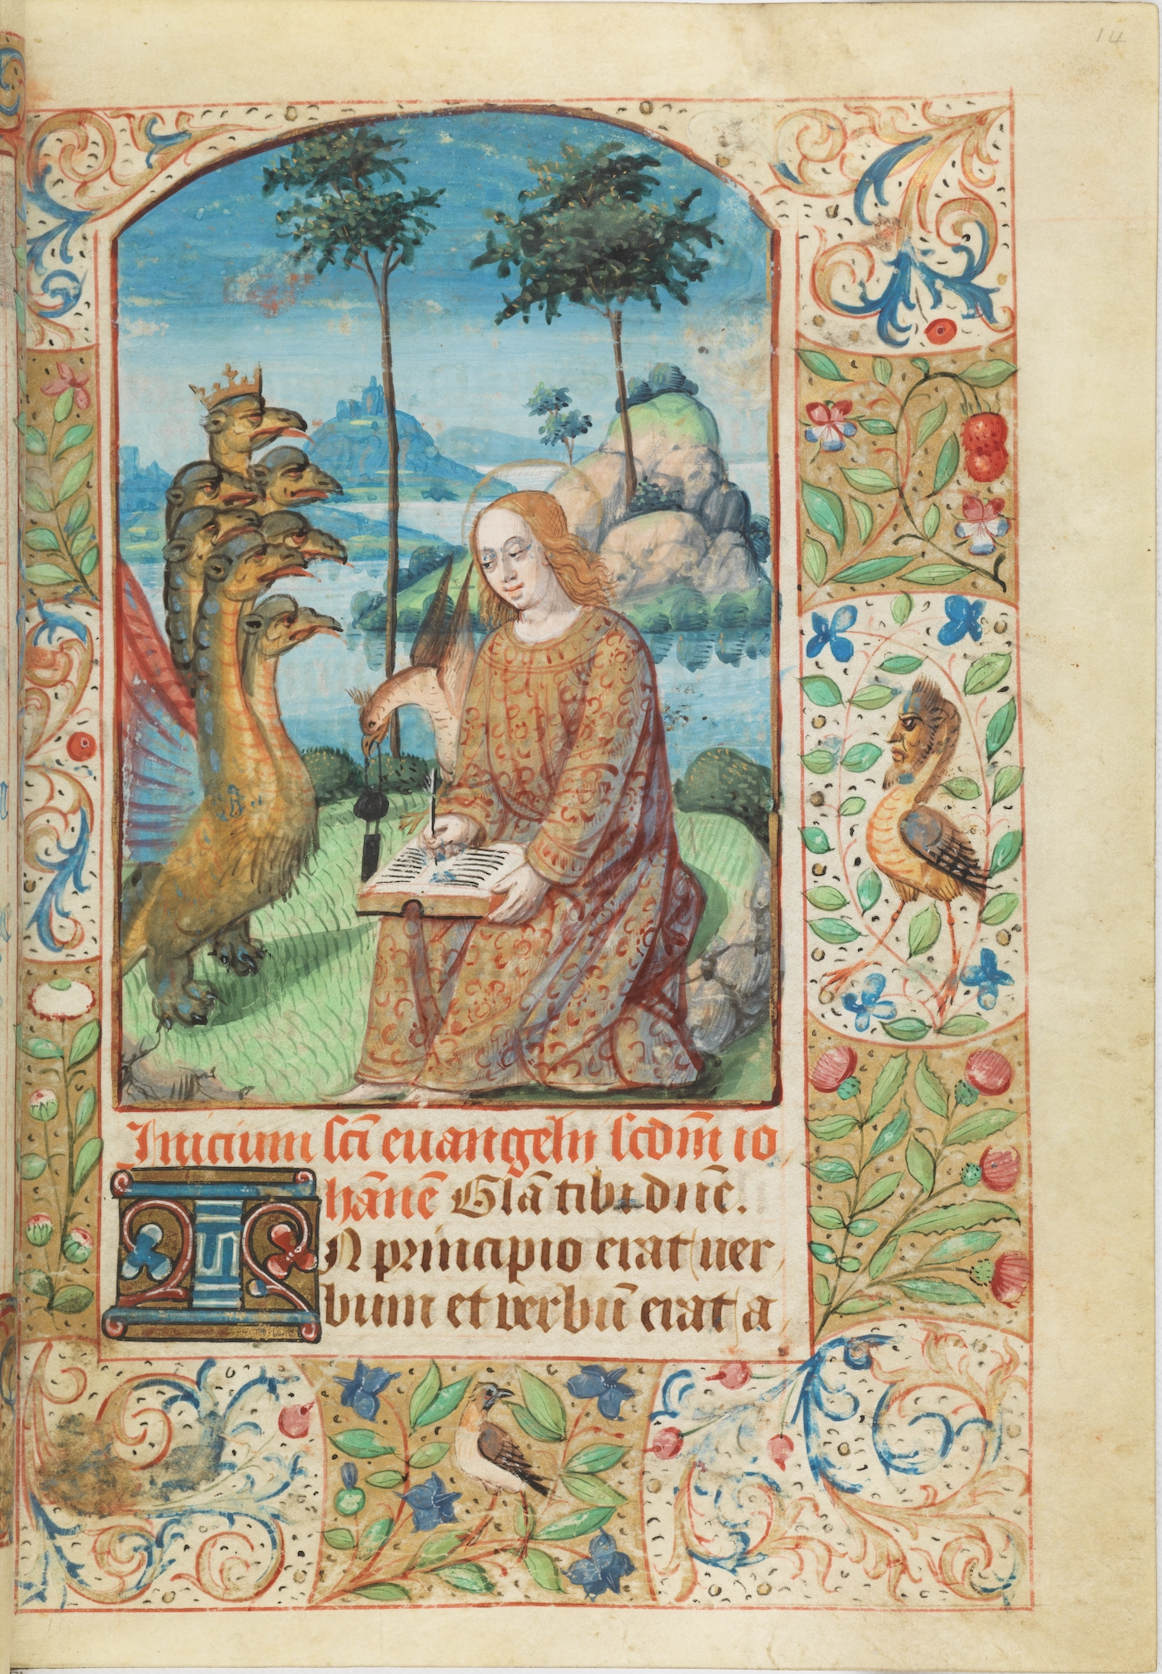
\includegraphics[width=\textwidth]{IMG_1a.png}
    \end{minipage}
    \hfill
    \begin{minipage}[b]{0.45\textwidth}
        \centering
        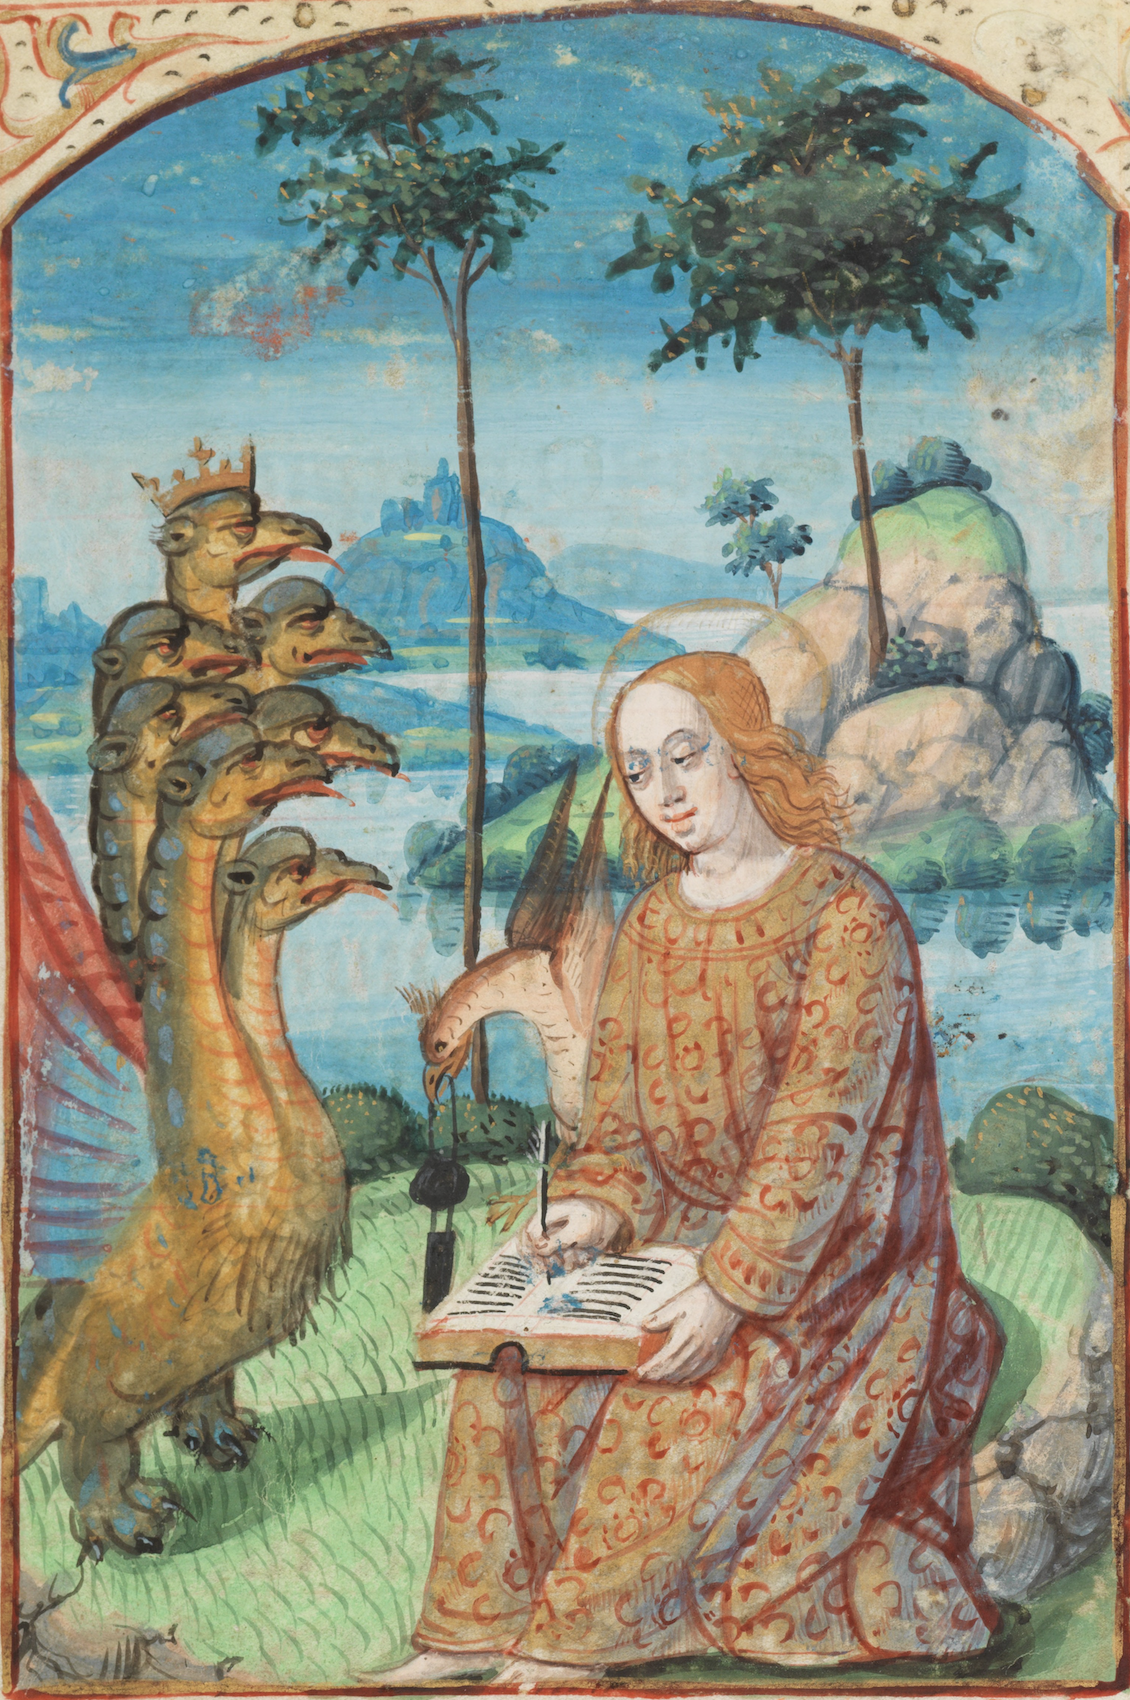
\includegraphics[width=\textwidth]{IMG_1b.png}
    \end{minipage}
    \caption{Genève, Bibliothèque de Genève, Livre d’heures de Philibert de Viry à l’usage de Genève (Ms. lat. 367), f°14r : l’image de gauche pour rechercher les miniatures et celle de droites les livres (\url{https://www.e-codices.unifr.ch/fr/mirador/bge/lat0367/bge-lat0367_014r}}.
\end{figure}

Il est également indispensable de présenter différents niveaux de complexité. Cela implique une variation d’angles (de face, côté), de niveaux d’occultation (objet tronqué par un élément extérieur), tout en gardant une certaine homogénéité. \\

Enfin, un \textit{dataset} doit être suffisamment important pour permettre à l'algorithme un apprentissage profond des objets à détecter. Le nombre de données disponibles est souvent l’un des enjeux clé pour obtenir un modèle robuste. Il est nécessaire de prendre en compte que la recherche d’exhaustivité ne doit pas se faire au détriment de la multiplicité des données et de leur qualité. 

\subsection{Jeux de données utilisés}

Le jeu de données ‘\textit{Coat of Arms’} a été conçu par l’équipe du laboratoire \textit{Digital History}, nous n’avons pas participé à sa conception. Celui-ci se compose de manuscrits européens ornés de représentations héraldiques, dont une partie importante d’armoriaux.
Les jeux de données ‘Miniatures’ et ‘\textit{Books in books}’ ont été conçus à partir des livres d’heures sélectionnés et des données collectées dans le cadre du projet HORAE \footnote{\url{https://github.com/oriflamms/HORAE/blob/master/Corpus/BooksOfHours_MSS_Manifests.csv}} La présente liste est basée sur un recensement plus large des livres d'heures et se limite aux manuscrits numérisés entièrement disponibles par le biais de l'IIIF. Nous avons sélectionné les manuscrits dont au moins un des folios contient une miniature.\\

Les 480 folios qui composent le jeu de données ‘Miniatures’ ont été sélectionnés aléatoirement dans un corpus déjà existant \footnote{\url{https://demo.arkindex.org/browse/cd38d0a4-bfd6-4bef-a44f-1d4da09226fd?type=illustration\&order=random }}. Dans le cadre de l’entraînement que nous avons mis en place, il nous importait de pouvoir entraîner un modèle à détecter des miniatures sans autres contraintes que celle de la présence de cycles iconographiques au sein de manuscrits comportant du texte et des images, le plus souvent les deux sur un même folio. Il n’y a donc pas nécessité d’avoir une pluralité de types de représentations puisqu'il s’agit de séparer les cycles iconographiques du texte. En revanche, toutes les données choisies présentent, à minima, une miniature. \\

Le \textit{dataset }‘\textit{Books in books}’ a été conçu à partir du même corpus que celui dont est issu le \textit{dataset} ‘Miniatures’. Dans le cadre de ce jeu de données, nous avons sélectionné manuellement les miniatures dans lesquelles au moins un support d’écriture est présent : codex, phylactère ou rouleau. Nous nous devions d’avoir une représentativité la plus homogène possible des différents types de supports d’écritures que nous cherchions à détecter (\textit{codices}, phylactères, rouleaux). Malheureusement, la représentation naturelle des différents supports est très variable, avec une forte présence de \textit{codices} par rapport aux autres supports. Ainsi, notre jeu de données se compose de 495 miniatures, qui ne sont pas systématiquement les mêmes que celles du jeu de données ‘Miniatures’

\paragraph{Conclusion}Chacun des \textit{datasets} a été pensé et construit de manière précise, dans le but de répondre à des questionnements spécifiques afin de former les modèles les robustes, fiables et les moins biaisés possibles. Toutes les données ont été collectées depuis des manifestes IIIF. 

\section{Les standards IIIF et le traitement automatisé des données}
\subsection{Principes et intérêts des standards IIIF pour la collecte de données historiques}

IIIF -- \textit{International Image Interoperability Framework} -- est une spécification technique qui permet de diffuser, présenter et annoter des images et documents numériques \footnote{\url{https://iiif.io/ }}. Ce standard a été conçu pour pallier le manque d’interopérabilité entre les différentes institutions patrimoniales. Il offre un accès unifié à un ensemble de données numériques sur les documents anciens et permet de visualiser, de consulter et d'interroger des manuscrits numérisés, des catalogues et des bases de données spécialisées sur divers aspects de l'étude du patrimoine écrit. L’intérêt pour le traitement automatisé des images dans le cadre d’une recherche sur les sources iconographiques médiévales fondée sur la \textit{computer vision}, repose sur l’API Image, permettant de récupérer facilement les méta-données techniques, et surtout sur l’API Présentation de IIIF. \\

L’API Présentation constitue à la fois un format d’échange, structuré en JSON-LD, et un modèle décrivant la représentation numérique d’un objet. L’API Présentation permet donc de spécifier les méta-données descriptives, structurelles (en particulier la liste ordonnée des images qui le constitue, leurs identifiants et leurs dimensions en pixels) et techniques des objets numériques -- dans le cadre de notre problématique les manuscrits -- dans un fichier appelé manifeste. Ainsi, les manifestes IIIF, offrent de précieux avantages pour le traitement des manuscrits médiévaux. En particulier pour la collecte et l’organisation des données grâce leur structure standardisée qui permet de collecter les données depuis différentes institutions et un traitement industrialisé des collections de manuscrits numérisés.

\subsection{Spécificités IIIF pour les manuscrits médiévaux}

La standardisation des manifestes et de leur format, permet la mise en place de scripts de téléchargements automatisés pour constituer dans le même temps des jeux de données et une bibliothèque virtuelle avec des manuscrits issus de multiples institutions répartis dans différents pays. 
Selon la spécification IIIF, un manifeste décrit la structure et la disposition d'un objet numérisé, notamment celle des folios. Sur la base du modèle de données \textit{Shared Canvas} \footnote{\url{http://iiif-io.us-east-1.elasticbeanstalk.com/model/shared-canvas/}}, un manifeste a la structure suivante : \\
\begin{itemize}
    \item Une ou plusieurs séquences,
    \item Chaque séquence (ordre des vues) doit comporter au moins un canevas,
    \item Chaque canevas (conteneur virtuel) doit avoir une ou plusieurs ressources de contenu (telles que des images ou des textes dans un manuscrit). L'association des images à leurs canevas respectifs se fait par le biais d'annotations. 
\end{itemize}

\paragraph{Conclusion}Dans le cas spécifique des manuscrits médiévaux, chaque canevas contient l’image d’un folio. Cette spécification IIIF  nous permet de collecter dans le même temps les images et leurs métadonnées.

\subsection{Stratégie de téléchargement des manuscrits à partir des manifestes IIIF}

La normalisation des manifestes facilite grandement le développement de code pour la récupération et la gestion d'images, car il peut être conçu de manière générique pour interagir avec des manifestes IIIF provenant de diverses sources, tout en garantissant une cohérence dans la manière dont les données sont extraites et conservées. En nous appuyant sur la structure normée des manifestes nous avons pu mettre en place un pipeline de téléchargement \footnote{\url{https://github.com/Chaouabti/Memoire_TNAH_2023/blob/main/Training\_model\_workflow/0\_Download\_processing.ipynb}}. En parcourant les canevas de la séquence du manifeste, le code permet, pour chaque image, d’extraire le label du canevas, l'URL de l'image et son format. Ces informations sont utilisées pour générer un nom de fichier unique en combinant le nom du manifeste, le numéro du canevas et l'extension du fichier image. Cela garantit que toutes les images téléchargées sont stockées au même format, simplifiant ainsi la gestion ultérieure.

\newpage
Nous avons également pu automatiser le processus de téléchargement en soumettant comme paramètre d’entrée une liste de manifestes dans un CSV à deux colonnes : la première contenant l’URL du manifeste, la seconde le nom du manuscrit. \\

\begin{verbatim}
'''EXAMPLE OF CSV file:x
'''
'''
Image_basename;Manifest_URL
MS Typ 1006;https://fragmentarium.ms/metadata/iiif/F-y5pq/manifest.json
MS Lat 451;https://fragmentarium.ms/metadata/iiif/F-j8m5/manifest.json
'''

\end{verbatim}

Pour la construction des jeux de données ‘Miniatures’ et ‘\textit{Books in books}’, nous avons créé un script dédié qui prend en entrée le CSV des miniatures du projet HORAE \footnote{\url{https://github.com/Chaouabti/Memoire\_TNAH\_2023/blob/main/Data/Export\_stutzmann\_horae\_t98\_image\%20zone.csv}}. Pour chaque miniature, c’est-à-dire chaque ligne du CSV, l’image du folio a été téléchargée intégralement à partir des données contenues dans la colonne [‘image\_URL’] et le folio entier en remplaçant les coordonnées de la boîte d’annotation. Les coordonnées absolues des boîtes d’annotations sont directement indiquées dans l’URL de la miniature. L’API Image de IIIF spécifie une syntaxe URL normalisée pour la transmission d'une image par le biais d'une requête HTTP standard. Cette syntaxe s'applique à deux types de demandes différentes pour la même image : la demande de l'image elle-même (fichier image) et la demande d'informations techniques sur l'image (fichier JSON). Le modèle d'URL pour demander une image doit être conforme au modèle d'URL suivant :
 
\begin{center}
    \makebox[\textwidth][c]{\small
    \texttt{\{scheme\}://\{server\}/\{prefixe\}/\{identifiant\}/\{région\}/\{taille\}/\{rotation\}/\{qualité\}.\{format\}}}
\end{center}
 
Ainsi en remplaçant les coordonnées de la région, par ‘full’ afin de récupérer l’image dans son ensemble, nous pouvons télécharger directement le folio.

\newpage
\begin{figure}[ht]
    \centering
    \begin{minipage}[b]{0.45\textwidth}
        \centering
        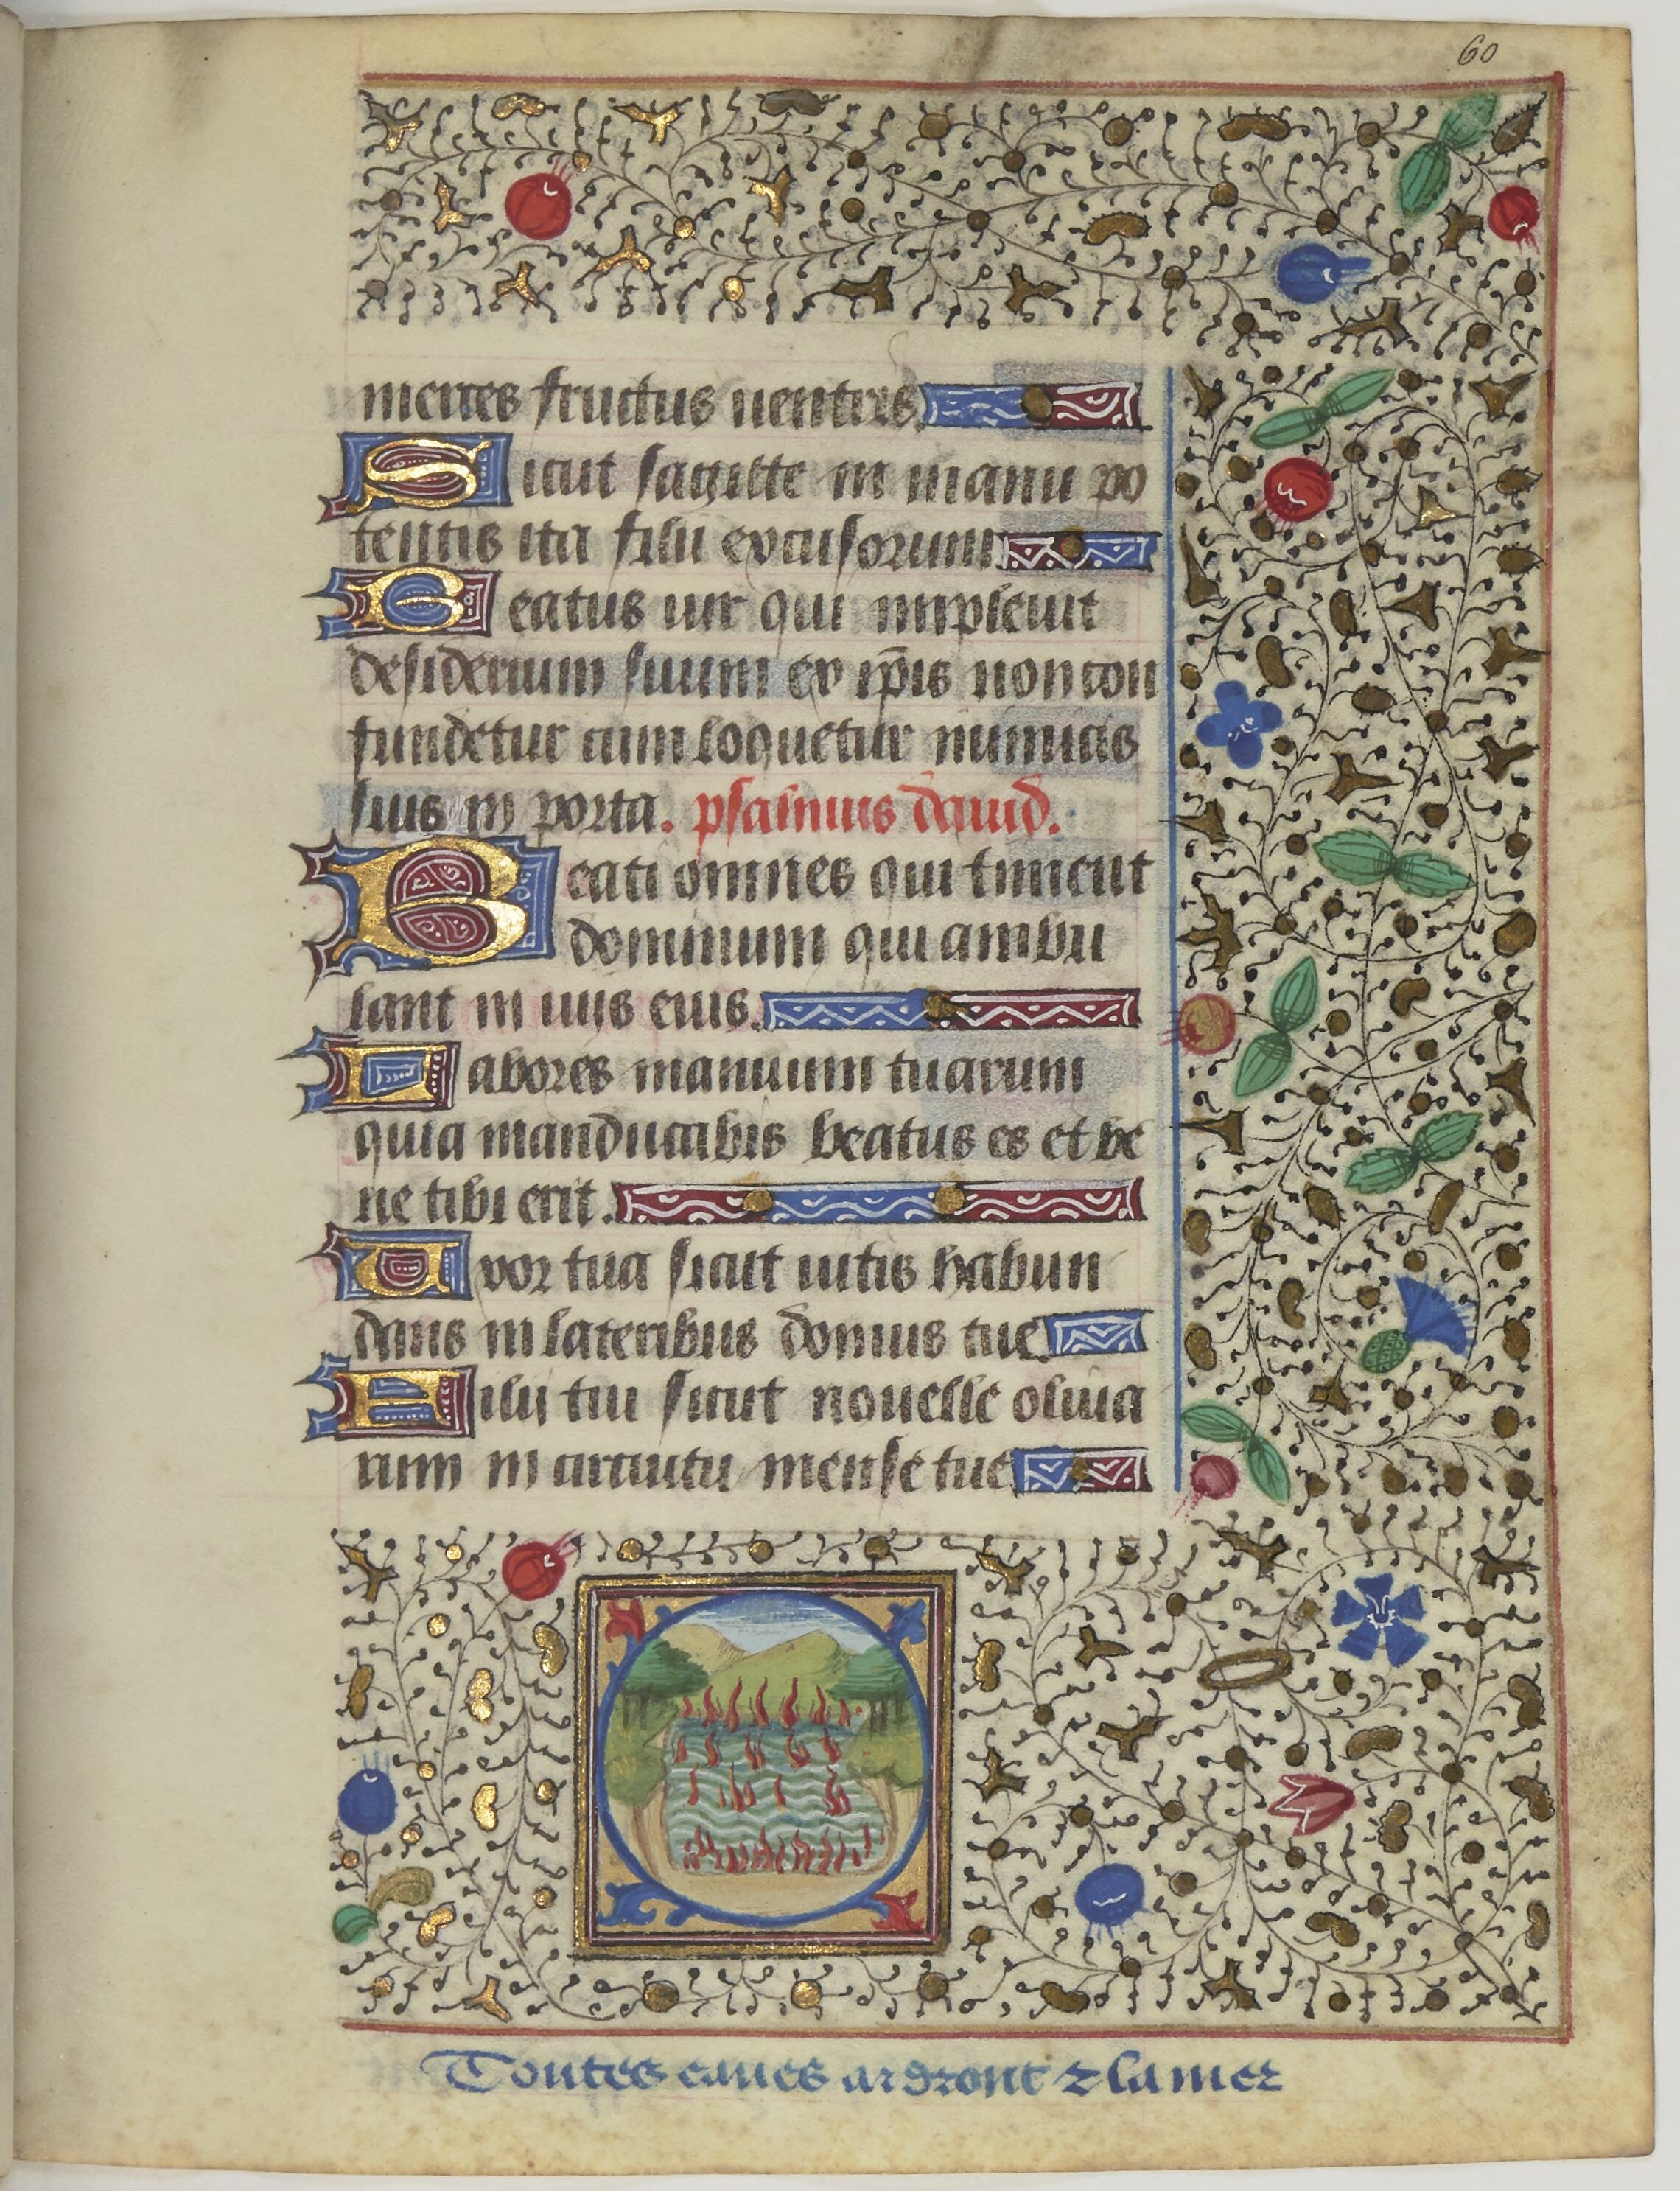
\includegraphics[width=\textwidth]{Exemple_IMG_FULL.jpg}
        \caption{\url{https://gallica.bnf.fr/iiif/ark:/12148/btv1b10527644s/f127/full/full/0/default.jpg}}
    \end{minipage}
    \hfill
    \begin{minipage}[b]{0.45\textwidth}
        \centering
        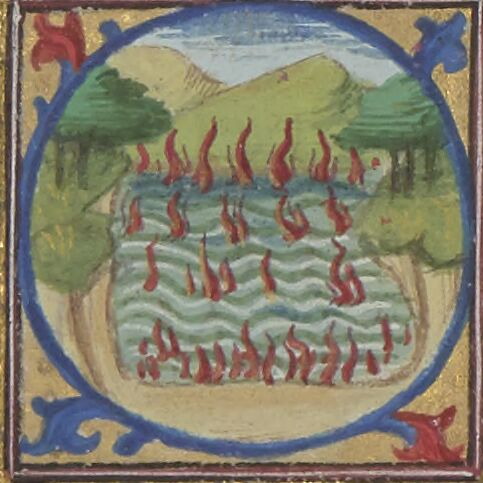
\includegraphics[width=\textwidth]{Exemple_IMG_NOT_FULL.jpg}
        \caption{\url{https://gallica.bnf.fr/iiif/ark:/12148/btv1b10527644s/f127/790,2158,483,483/full/0/default.jpg}}
    \end{minipage}
\end{figure}

Ces deux approches fonctionnent grâce au standard IIIF, qui permet également la production, en parallèle du téléchargement, de fichiers contenant les métadonnées des images téléchargées. Les modifications que nous avons apportées au script préexistant étendent les fonctionnalités afin de gérer des ensembles de manifestes, documenter les téléchargements et conserver les métadonnées des différentes images dans des fichiers CSV. Ceux-ci seront utilisés dans la suite du traitement des données, en particulier pour évaluer la robustesse des modèles entraînés. 

\subsection{Collecte des métadonnées}

Après téléchargement chaque manuscrit fait l’objet de la création d’un dossier dont le nom est celui indiqué dans la colonne ‘name’ du CSV. Pour chaque manuscrit les images sont conservées dans un dossier au nom du manuscrit contenant le manifeste IIIF, les images et un fichier CSV éponyme suivi de ‘\_image\_data.csv’.  Le fichier CSV contient les métadonnées de chacune des images du manifeste, qu’elle soit téléchargée ou non. Cela inclus l'URL du manifeste, l'ID du canevas, l'URL de l'image, le chemin absolu du dossier créé pour stocker les images téléchargées, le nom de l'image tel qu'il est déclaré dans le manifeste, la largeur et la hauteur de l'image telle qu'elles sont déclarées dans le manifeste et le code HTML pour vérifier si l'image a bien été téléchargée. Si l’image est correctement téléchargée, le code HTML est 200 et les données de l’image téléchargée sont indiquées : le nom du fichier (nom du dossier/fichier image), les dimensions de l’image téléchargée, c’est-à-dire sa largeur et sa hauteur. \\

La conservation de ces données permet de savoir exactement qu’elles sont les données disponibles et leurs caractéristiques. Par exemple, le suivi du téléchargement des images et la possibilité de relancer le script de téléchargement si des images venaient à manquer sans retélécharger l’ensemble des images du manifeste grâce au code HTML conservé dans le fichier CSV.Pour le téléchargement des images HORAE présentent dans le fichier‘Export\_stutzmann
\_horae\_t98\_image zone.csv’, les méta-données conservées sont identiques à celles téléchargées depuis un manifeste IIIF. Pour la conservation des coordonnées des miniatures et pouvoir les traiter plus facilement par la suite, une colonne avec les coordonnées relatives, appelée ‘relative\_coordinates’, a été créée et contient : \\
\begin{itemize}
    \item Le numéro de la classe (toujours 0 puisque le modèle à entraîner doit détecter uniquement les miniatures)
    \item -	La valeur x du centre de la \textit{bounding box}, la valeur y du centre de la \textit{bounding box}, la largeur relative et la hauteur relative. 
\end{itemize}

\paragraph{Conclusion}La mise en place et la constitution du jeu de données est cruciale pour un traitement automatisé par computer vision. Dans le cadre d’un travail sur les manuscrits médiévaux l’utilisation des données au format IIIF joue un rôle crucial pour le recollement, le traitement et la conservation des données. Dans le cadre du stage effectué au sein du laboratoire \textit{Digital History} nous avons adapté le code de téléchargement déjà mis en place par l’équipe scientifique de manière à automatiser les processus de téléchargement et à conserver les méta-données des images que nous utiliserons pour l’entraînement des modèles et pour l’inférence. 

\section{Annotations des données}
\subsection{Annoter des données historiques : principes}

Un des enjeux de l’annotation repose sur la cohérence sémantique dans les annotations et explication de la documentation de l'ontologie. La procédure d'annotation se doit d’être conçue de sorte à être la plus harmonieuse possible. Cela implique trois notions essentielles que sont la cohérence, la précision et l’exhaustivité. \\

La cohérence, de sorte que l'annotation des images soit homogène en termes de définition des classes (éviter les notions trop vagues), de placement des boîtes de délimitation (laisser un espace entre l’objet annoté et la boîte d’annotation) et de définition des points de vue et de la troncature (faut-il annoter l’objet s’il est tronqué par un autre élément iconographique ou s’il sort du cadre de l’image). La précision, de sorte que le nombre d'erreurs d'annotation soit aussi faible que possible, et l’exhaustivité, de sorte que toutes les instances d'objets soient étiquetées. Dans la mesure du possible, l'ensemble des objets annotés doivent être inclus dans la \textit{bounding box}. Idéalement, une petite zone autour de l’objet devrait également être incluse dans la boîte d'annotation. De cette manière, le modèle est mieux entraîné à reconnaître les limites des éléments de l'image. Chaque élément doit scrupuleusement être annoté, y compris si les boîtes d’annotations se chevauchent. Par ailleurs, si une partie de l’objet à annoter est en partie recouvert par autre chose, la partie recouverte devrait également se trouver dans la \textit{bounding box}. De même, Si des éléments d'image à annoter se trouvent en partie en dehors du scan, ils devraient tout de même être annotés dans la mesure où ils sont visibles \footcite{everingham_pascal_2010}.\\



\subsection{\textit{Label Studio}}

Pour l’annotation des différents \textit{datasets} nous avons utilisé l’outil d’étiquetage \textit{Label Studio}, anciennement \textit{LableImg} \footnote{\url{https://labelstud.io}}. Les avantages de cet outil sont la compatibilité avec différents formats de données de boîtes englobantes, une interface utilisateur simple et la possibilité d’extraire les données directement utilisables pour un entraînement YOLO.\\

Par ailleurs, il est également possible de modifier directement les boîtes d’annotations générés par YOLO. Dans cette perspective les scripts ont été conçus pour pouvoir charger les images, les annoter et les corriger qu’elles soient conservées localement ou accessible en ligne. L'annotation se fait sur un serveur local et les données d'exports contiennent :
\newpage
\begin{itemize}
    \item Un fichier ‘notes.json’ : contenant sous la forme d'un dictionnaire les différentes classes annotées. La clé correspond au numéro de label d'une classe (int) et la valeur est le nom de la classe (str).
    \item Un fichier classes.txt : contenant une liste les différentes classes sans leur code (une classe par ligne) ;
    \item Un dossier labels contenant des fichiers 'txt':
    \begin{itemize}
        \item Un fichier par image (le même nom que l'image annotée, seul l'extension .txt change)
        \item Chaque fichier contient le numéro de la classe annotée et les coordonnées relatives des boîtes d’annotations. 
    \end{itemize}
    \item Un dossier images contenant toutes les images annotées sans les \textit{bouding boxes} au format .jpg.
\end{itemize}

\paragraph{}
Chaque \textit{bounding box} est représentée par une ligne. Ainsi, chaque fichier ‘.txt’ contient autant de ligne de que boîtes d’annotions, c’est-à-dire d’objets à détecter dans l’image. Les colonnes représentent respectivement :
\begin{itemize}
    \item Le code de la classe (de 0 à x),
    \item Les coordonnées relatives de la \textit{bounding box} qui indiquent la position de la box dans l'image au format x,y,w,h :
    \begin{itemize}
        \item x: indique la position horizontale du centre de la \textit{bounding box},
        \item y : indique la position verticale du centre de la \textit{bounding box},
        \item w (weight) : la largeur de la \textit{bounding box} par rapport à la largeur totale de l'image,
        \item h (height) : la hauteur de la \textit{bounding box} par rapport à la hauteur totale de l'image.
    \end{itemize}
\end{itemize}

Ces coordonnées doivent être normalisées en fonction des dimensions de l'image (c'est-à-dire avoir des valeurs comprises entre 0 et 1). Les numéros de classe sont indexés par zéro.

\paragraph{}
Il est important de noter que \textit{Label Studio} modifie les noms des fichiers lors de la récupération des données au format YOLO. La modification consiste en l’ajout d’une série aléatoire de 8 chiffres ou lettres et d’un ‘-’. Il est nécessaire de modifier les nom des fichiers .txt et des fichiers images.

\newpage
\subsection{Générer des annotations depuis l'URL des images}

Les coordonnées des miniatures telles sont indiquées dans l’URL ont été utilisées pour générer des annotations pour chaque image sous la forme d’un fichier .txt de sorte que :
\begin{itemize}
    \item Le fichier a exactement le même nom que l’image à laquelle il est lié (seule l’extension change)
    \item Il contient :
    \begin{itemize}
        \item Le code de la classe miniature (par défaut 0),
        \item Les coordonnées relatives de la \textit{bounding box}
    \end{itemize}
\end{itemize}


\paragraph{}
 Seule une transformation des coordonnées des miniatures depuis {taille} en valeurs relatives a été effectuée. Ainsi, les fichiers .txt créés peuvent être utilisés tels quels pour l’apprentissage YOLO. Pour chaque image annotée un fichier ‘txt’ a été généré portant le même nom que l’image contenant les coordonnées de la ou des boîtes d’annotations de chaque miniature. \\

 \paragraph{Conclusion}L’annotation est une étape clé et fondamentale pour l’entraînement et la robustesse des modèles entraîné. Une vérité terrain homogène accroît la robustesse des modèles entraînés. Label Studio est un outils particulièrement efficace pour l'annotation de données en vue d'un entraînement YOLO. Il est tout aussi judicieux d'envisager d'autres traitements pour l'annotation des données si celles-ci sont pertinents.

 \section{Conclusion}

La construction du \textit{dataset} doit donc répondre à des critères simples mais essentiels que sont la diversité et la pluralité des données. L’utilisation de données issues de manifestes IIIF représente un véritable atout pour la construction de jeu de données historiques utilisées dans le cadre d’une analyse par \textit{computer vision} grâce à la facilité de recollement et de conservation des métadonnées. Enfin, l’annotation des données, qui repose en grande partie sur l’ontologie doit garantir un jeu de données cohérent pour créer les modèles les plus robustes possibles. Chacun des \textit{datasets} a été pensé et construit de manière précise, dans le but de répondre à des questionnements spécifiques afin de former les modèles les robustes, fiables et les moins biaisés possibles. Toutes les données ont été collectées depuis des manifestes IIIF.

 \chapter{Analyse des données d'entraînement et production de modèles}

Dans ce chapitre nous analyserons les données utilisées pour l’entraînement des premiers modèles et nous présenterons la construction des \textit{datasets} d’entraînement et de validation puis les paramètres choisis pour les différents entraînements.  

\section{Analyse des données d’entraînement}
\subsection{Principes d'analyse}

Le nommage normalisé des images téléchargées permet de facilement analyser et comprendre la structure des données utilisées pour former les différents modèles. Dans cette perspective nous avons inclus dans le traitement des données des scripts permettant d’analyser la répartition des données \footnote{\url{https://github.com/Chaouabti/Memoire_TNAH_2023/blob/main/Training_model_workflow/1_Statistics_for_training_data.ipynb}}. Tous ces scripts sont conçus pour traiter des données images et textes de même nom (à l'exception de l'extension) contenus dans deux dossiers, l'un nommé 'labels' avec tous les fichiers .txt et l'autre 'images' avec toutes les images. Les résultats obtenus devraient permettre d'évaluer la pertinence des corpus utilisés pour les différents entraînements et d'étudier les raisons de la robustesse ou la faiblesse du modèle.\\

Pour analyser les données nous avons choisi d’explorer la répartition des images par manuscrits, le nombre d’annotations par image et la distribution des classes annotées. Les résultats de chacune de ces données sont conservés dans des fichiers CSV, nommés respectivement ‘img\_per\_ms.csv’, ‘annotations\_per\_img.csv’ et ‘class\_distribution.csv’. La connaissance des répartitions est essentielle pour cerner les biais qui pourraient exister dans l’entraînement des modèles, comme une sur-représentation d’une classe par rapport aux autres ou une trop grande hétérogénéité quant à l’origine des images. Le nombre d’annotations par image permet de s’assurer de la diversité des cas qui peuvent exister quant à la présence multiple d’objets d’une même classe dans une seule image. \\

Enfin, nous pouvons avoir une vue d’ensemble grâce au fichier nommé ‘global\_data.csv’ qui nous renseigne sur le nombre de manuscrits dont sont issues les images, le nombre de d’images non annotées et le nombre total d’annotations.

\subsection{Description des jeux de données d'entraînement}

\subsubsection{Jeux de données \textit{Coat of Arms}}

Les données du \textit{dataset} \textit{Coat of Arms} correspond au jeux de données ‘train\_group\_7’ du laboratoire \textit{Digital History} et se compose de 2498 images, issues de 136 manuscrits différents. 

\begin{figure}[ht]
    \centering
    \begin{minipage}[b]{0.45\textwidth}
        \centering
        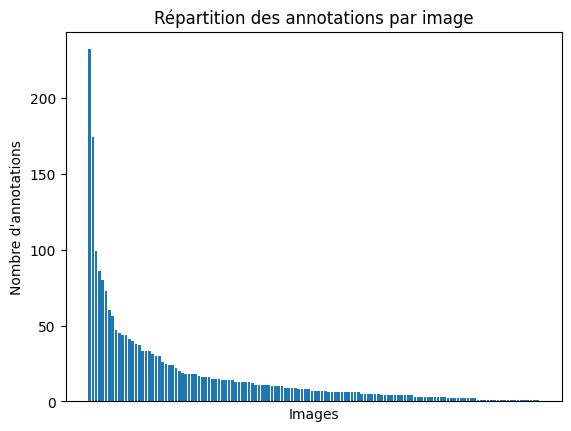
\includegraphics[width=\textwidth]{IMG_training_group_7_Annotations_per_img.png}
        \caption{Annotations par images pour le \textit{dataset Coat of Arms}}
    \end{minipage}
    \hfill
    \begin{minipage}[b]{0.45\textwidth}
        \centering
        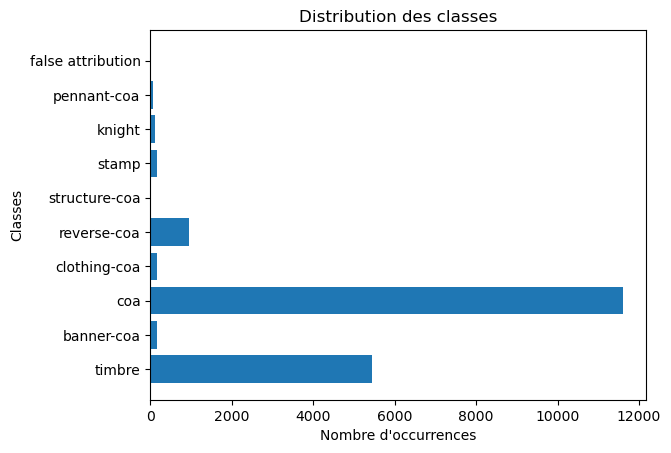
\includegraphics[width=\textwidth]{class_distribution_COA.png}
        \caption{Distribution des classes d'annotation pour le \textit{dataset Coat of Arms}}
    \end{minipage}
\end{figure}

Le nombre d’images par manuscrit est très hétérogène, allant de 232 à 1. Près de 57\% des manuscrits présentent moins de 10 images et plus de 25\% du corpus est représenté par 5 manuscrits (armoriaux datés entre la seconde moitié du XVe siècle et le XVIIe siècle). Seules 94 images ne sont pas annotées. De même que le nombre d’images par manuscrit est très hétérogène, la répartition des annotations varie de 110 à 0. \\

Malgré un nombre important de classes d’annotations, 91\% du corpus est représenté par deux classes : coa 62\% et timber 29\%. La surreprésentation de ces deux classes est liée à la nature même du \textit{dataset} initial issu en grande partie des armoriaux où sont représentées les armes des familles sur des boucliers et des heaumes. 

Sur les 9\% de données non annotées comme timber ou coa, plus de la moitié est représentée par la classe reverse-coa. Cela signifie que 7 des 10 classes concernent moins de 5\% du \textit{dataset}. S’il est très dangereux d’anticiper les résultats d’un entraînement, il est tout de même possible d’envisager les problématiques engendrées par la disparité et la grande variabilité dans le jeu de données COA. La sur-représentation de certaines classes et la quasi-absence d’autres, risque d’entraîner une grande disparité dans la robustesse du modèle qui sera plus à même à détecter certaines classes et d’en omettre d’autres. 

\subsubsection{Jeu de données Miniatures}

Le jeu de données ‘Miniatures’ se compose de 480 images issues de 143 manuscrits différents.

\begin{figure}[ht]
    \centering
    \begin{minipage}[b]{0.45\textwidth}
        \centering
        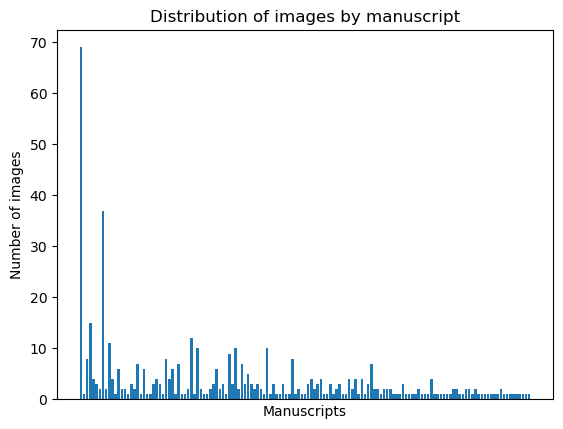
\includegraphics[width=\textwidth]{img_per_ms_Miniatures.png}
        \caption{Annotations par images pour le \textit{dataset} Miniatures}
    \end{minipage}
\end{figure}

Ce jeu de données ‘Miniatures’ ne présente qu’une classe d’annotation et une provenance homogène, à l’exception de deux manuscrits dont est issu près d’un quart du\textit{ dataset} (112 images).

\newpage
\subsubsection{Jeu de données \textit{Books in books}}

Le jeu de données ‘\textit{Books in books}’ se compose de 495 images issues de 136 manuscrits différents.

\begin{figure}[ht]
    \centering
    \begin{minipage}[b]{0.45\textwidth}
        \centering
        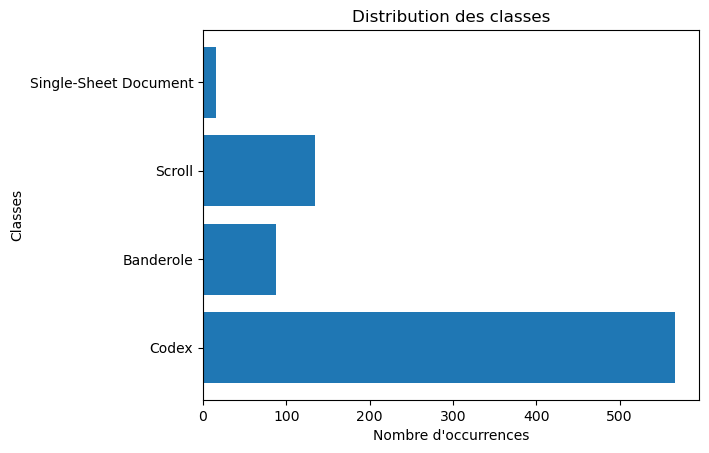
\includegraphics[width=\textwidth]{class_distribution_BiB.png}
        \caption{Annotations par images pour le \textit{dataset Books in books}}
    \end{minipage}
    \hfill
    \begin{minipage}[b]{0.45\textwidth}
        \centering
        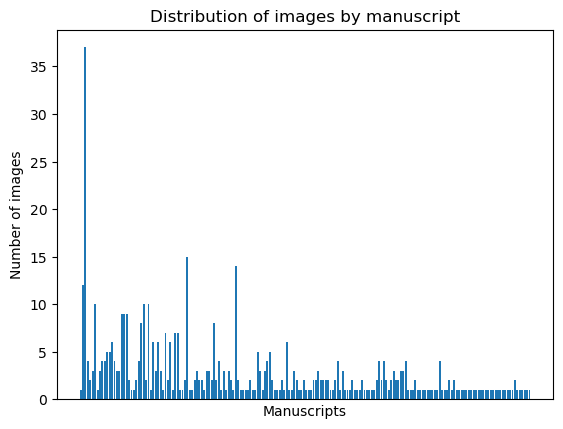
\includegraphics[width=\textwidth]{img_per_ms_BiB.png}
        \caption{Distribution des classes d'annotation pour le \textit{dataset Books in books}}
    \end{minipage}
\end{figure}

Le jeu de données ‘\textit{Books in Books}’ est peu étendu (moins de 500 images et 805 annotations). Les différentes classes ne sont pas toutes aussi bien représentées avec une prépondérance de la classe codex (567 des 805 annotations). Certaines classes minoritaires, comme ‘\textit{Scroll}’ ont été ciblées vers la fin de l'opération d'annotation afin d'en augmenter le nombre. Il s'est avéré impossible de collecter des exemples de certaines classes, comme les ‘\textit{Horn Book}’ et ‘\textit{Woden tablet codex}’, en raison de l'absence total d’objet relevant de l’une ou l’autre de ces deux classes dans les miniatures explorées. 

\paragraph{Conclusion} Malgré notre volonté d’avoir une représentation équilibrée et homogène des classes d’annotations, nos différents jeux de données présentent une forte hétérogénéité en raison de la nature même des corpus dont ils sont issus. Il nous importera donc de commenter les impacts de cette disparité de représentation des classes sur la qualité des modèles entraînés.

\newpage
\section{Répartition des données et spécifications YOLOv8}

\subsection{Répartition des données d'entraînement}

La répartition des données d'entraînement est une étape essentielle dans le processus de préparation des données pour l'apprentissage automatique (\textit{machine learning}). Cette répartition consiste à diviser l'ensemble des données en plusieurs ensembles distincts pour différentes phases de l'apprentissage automatique, répartis généralement de la manière suivante : \\
\begin{itemize}
    \item Un ensemble d’entraînement (\textit{train}) : ensemble des données à partir duquel le modèle apprend et affine ses paramètres pour effectuer des prédictions. Il représente la majorité des données annotées.
    \item Un ensemble de validation (\textit{val}) :  cet ensemble permet d’ajuster les hypermètres du modèle.
    \item Un ensemble de test : cet ensemble est utilisé pour évaluer la performance finale du modèle. Il se constitue de données que le modèle ne connaît pas et permet donc de juger la capacité du modèle à analyser et prédire la présence des objets sur des données neuves. A l’inverse des deux ensembles précédents, celui-ci est facultatif. 
\end{itemize}

\paragraph{}Il n’existe pas de règle précise quant à la répartition des données dans ces différents ensembles, des ajustements sont nécessaires en fonction de la quantité des données à disposition. Lors de notre arrivée dans le laboratoire \textit{Digital History}, la pratique était une division 70/20/10, où 70\% des données sont utilisées pour l'entraînement, 20\% pour la validation et 10\% pour le test. Pour le \textit{dataset Coat of Arms} nous avons conservé cette répartition. Pour les jeux ‘Miniatures’ et ‘\textit{Books in books}’, en raison de la taille restreinte des jeux de données, nous n'avons pas créé d’ensemble test et privilégié une répartition 80/20 (80\% pour l’entraînement et 20\% pour la validation). Nos tests ont été déployés directement sur des manuscrits – pour l’entraînement ‘Miniatures’ -- ou des miniatures -- pour le jeu ‘\textit{Books in books}’ -- en s’assurant au-préalable qu’aucune image n’a été utilisée pour l’entraînement des modèles respectifs. 

\newpage
\subsection{Spécifications de YOLOv8}

Par défaut, YOLOv8 attend que le chemin vers le dossier d’entraînement soit [CheminVersDossierRacine]/datasets. Les données d’entraînements sont envoyées dans un dossier éponyme (i.e. le nom du dossier dans lequel sont contenues les données). Les images sont envoyées dans un dossier ‘images’ et les fichiers d’annotations dans un dossier ‘labels’. Chacun de ces dossiers contient deux sous-dossiers contenant les données d’entraînement et de validation nommés respectivement ‘train’ et ‘val’. Nous avons automatisé la répartition des données dans les différents dossiers à partir de fichiers ‘txt’ : un nommé ‘traindata.txt’, contenant la liste des images utilisées pour l’entraînement, et un ‘valdata.txt’ contenant la liste des images utilisées pour la validation. Enfin, nous générons un fichier ‘training\_dataset’ contenant la liste des images utilisées pour l’entraînement et la validation\footnote{\url{https://github.com/Chaouabti/Memoire\_TNAH\_2023/blob/main/Training\_model\_workflow/2\_Data\_preparation\_and\_training.ipynb}}. Enfin, les fichiers sont déplacés dans les dossiers correspondants. La structure des dossiers contenant les données respecte les paramètres par défaut attendus par YOLOv8.\\

LLes détails de l'ensemble des données d’entraînement des modèles sont définis dans fichier ‘.yaml’, dont nous avons également automatisé la création. Celui-ci est requis pour que l’entraînement de modèle avec YOLOv8 puisse prendre en compte les chemins d’accès aux données ainsi que la répartition des différentes classes d’annotations. Pour YOLOv8, les informations doivent être structurée de la manière suivante :
\begin{center}
\begin{verbatim}
path: training_Dataset/
train: 'train/images'
val: 'val/images'

#class names
names:
  0: ' classe_0_name'
  1: ' classe_1_name'
  2: ' classe_2_name'  
  3: ' classe_3_name'

\end{verbatim}    
\end{center}

\newpage
Par défaut ce fichier doit se trouver dans le répertoire racine du projet, c’est-à-dire au même niveau que les dossiers ‘train’ et ‘val’.

\section{Paramètres d'entraînement}
\subsection{Les paramètres YOLO}

Les paramètres d'entraînement des modèles YOLO font référence aux différents hyperparamètres et configurations utilisés pour entraîner le modèle sur un ensemble de données. Ces paramètres ont une incidence sur les performances, la vitesse et la précision du modèle. Il est donc important d'ajuster et d'expérimenter soigneusement ces paramètres afin d'obtenir les meilleures performances possibles pour une tâche donnée. Nous ne commenterons pas ici l’ensemble des hypermètres modifiables mais seulement ceux que nous avons modifiés pour nos entraînements \footnote{La liste est disponible sur le site d’Ultralytics : \url{https://docs.ultralytics.com/modes/train/\#arguments}}. Nous avons concentré notre attention sur les paramètres suivants : \\
\begin{itemize}
    \item model : nom du modèle pré-entraîné pour répondre à différentes tâches et exigences de performance. Pour la détection il existe cinq modèle pré-entraînés yolov8n.pt, yolov8s.pt, yolov8m.pt, yolov8l.pt, yolov8x.pt. Chacun de ces modèles est plus puissant et plus lourd que le précédent. Si yolo8x.pt est le plus puissants des cinq modèles, il est aussi le plus lourd le plus susceptible de saturer la mémoire. 
    \item img-size : Ce paramètre correspond à la taille de l'image en pixels. Pour YOLO l'image doit être carrée, ainsi l'image originale est redimensionnée tout en conservant le rapport hauteur/largeur. Le côté le plus long de l'image est redimensionné à ce nombre. Le côté le plus court est complété par une couleur grise. Une plus grande résolution de l’image permet un entraînement plus robuste mais ralentit le processus et risque d’entraîner une saturation de la mémoire. 
    \item data : Le fichier Data YAML contient des informations sur l'ensemble de données : 
    \begin{itemize}
        \item le chemin d'accès aux images,
        \item le nombre d'étiquettes de classes,
        \item les noms des étiquettes de classe.
    \end{itemize}
    \item batch : La taille du batch correspond au nombre de paires image-caption propagées dans le réseau à un moment donné de la formation. 
    \item epochs : Nombre d'époques pour lesquelles la formation doit être effectuée. Cette valeur correspond au nombre total de passages de l'apprentissage du modèle sur l'ensemble du jeu de données.
    \item workers : Indique le nombre de processeurs alloués à l'apprentissage. Plus le nombre de workers est élevé plus l’apprentissage sera rapide. Il est important de noter qu’un nombre de workers trop élevé peut saturer la mémoire du GPU et interrompre le processus d’entraînement.
    \item name : Nom du dossier dans lequel les différents résultats de l'apprentissage, tels que les poids et journaux d'apprentissage, sont conservés.
    \item project : ce paramètre permet de contraindre YOLO à envoyer les données d’entraînement dans un dossier spécifique. Sans modification de ce paramètre les dossiers contenant les résultats d’entraînement et d’inférence sont envoyés dans le même dossier source. 
\end{itemize}

\paragraph{}Dans le cas d’une interruption non prévue de l’entraînement, il est possible de reprendre à la dernière époque (pour vérifier l’état d’avancement de l’entraînement, YOLOv8 produit un fichier results.csv dans le dossier runs/dataset\_name.) \\

Pour relancer un entraînement interrompu, il est nécessaire de conserver exactement les mêmes paramètres, à l’exception de : \\
\begin{itemize}
    \item model : indiquer le chemin d'accès au dernier poids, correspondant au fichiers 'last.pt' du dossier 'weights'
    \item resume : le paramètre doit être ajouté avec la valeur \textit{True} afin de reprendre à la dernière époque entraînée.
\end{itemize}

\subsection{Prévenir les risques}

Lors de l'apprentissage, un modèle peut être sous-adapté (\textit{underfitting}) ou suradapté (\textit{overfitting}).\\

L'\textit{underfitting} signifie que le modèle possède une faible capacité de prédiction en raison de l'impossibilité de capturer la complexité des données lors de l'apprentissage. Cela peut être dû à jeu de données trop restreint, une mauvaise représentation des différentes classes ou une vérité terrain mal préparée. Un mauvais paramétrage d’entraînement, un nombre insuffisant d’époques ou un taux d'apprentissage trop faible, peuvent également produire un modèle à capacité de prédiction réduite. 

\newpage
A l’inverse l’\textit{overfitting}, signifie que le modèle est trop adapté aux données d'apprentissage et ne parvient pas à faire des prédictions correctes sur de nouvelles données. YOLOv8 permet de suivre à chaque époque le taux d’erreur -- de perte -- (\textit{loss}), celui-ci devant diminuer au fur et à mesure des époques. Si la courbe stagne ou remonte, cela signifie que le modèle est surentraîné. Une des stratégies les plus efficace est l’augmentation des données d’entraînement : plus les exemples seront nombreux et différents, plus le risque d’avoir un modèle surentraîné diminue. \\

Ainsi, les paramètres autant que les jeux de données, doivent être pensés en amont ou ajustés au besoin. Un des avantages de YOLOv8 est la distinction entre le dernier modèle créé (qui correspond à la dernière époque entraînée) et le modèle le plus robuste (celui dont toutes les métriques sont les plus élevées). Il est donc recommandé d’utiliser pour l’inférence le meilleur modèle nommé ‘best.pt’. \\

Dans notre script d’entraînement nous avons déterminé ces différents paramètres de la manière suivante \footnote{\url{https://github.com/Chaouabti/Memoire\_TNAH\_2023/blob/main/Training\_model\_workflow/2\_Data\_preparation\_and\_training.ipynb}}:
\begin{center}
    \begin{verbatim}
        model = 'yolov8m.pt'
        img_size = 640 
        epochs = 100 
        batch = 8 
        workers = 24 
    \end{verbatim}
\end{center}

Ces arguments proposés "par défaut" sont ceux que nous avons évalués comme étant les plus équilibrés pour l'entraînement des différents modèles en ce qui concerne la robustesse, la limitation du risque de saturation de la mémoire et la vitesse. Il s'agit de suggestions plutôt que de recommandations, qui doivent être adaptées aux données et à la capacité de l'équipement utilisé.

\newpage
\subsection{Déploiement du modèle (inférence)}

L’inférence, ou prédiction, permet de déployer le modèle entraîné sur un jeu  de données que le modèle n’a pas encore vu, c’est-à-dire des données différentes de celles qui ont servi pour l’entraînement et la validation. De même que pour l’entraînement, l’inférence peut être paramétrée en fonction des données que l’on cherche à recueillir \footnote{L’ensemble des paramètres de l’inférence est consultable sur le site d’Ultralytics \url{https://docs.ultralytics.com/modes/predict/\#inference-arguments}}. Nous ne présenterons ici que les paramètres que nous avons modifiés :\\

\begin{itemize}
    \item model : chemin absolu vers le meilleur modèle entraîné (best.pt). 
    \item source: chemin vers le \textit{dataset} sur lequel appliqué le modèle.
    \item	save : par défaut le paramètre est \textbf{False} et ne produit pas de fichier de sortie avec les \textit{boudingboxes}. \textbf{True} permet de générer des images sur lesquelles les \textit{bounding boxes} sont indiquées. Ce paramètre peut être utile à activer si l’on souhaite avoir les annotations directement sur les images. A noter cependant que toutes les images sur lesquelles passent le modèle seront dédoublées, y compris celles sur lesquelles aucune détection n’aura été faite. 
    \item imgsz : indiquer la même taille que pour l'entraînement,
    \item name: dossier de sortie des résultats
    \item save\_txt=\textbf{True}: permet de conserver le fichier .txt avec les coordonnées des \textit{bounding boxes}. Les coordonnées des \textit{bounding boxes} sont conservées dans un dossier 'labels'. Ce dossier contient un fichier .txt pour chaque image analysée par le modèle et pour laquelle il existe une prédiction. Chaque fichier .txt contient une ligne par élément.
    \item save\_conf=\textbf{True}: permet de conserver le score de confidence de la détection dans le fichier .txt. Par défaut le paramètre est sur \textbf{False}.
    \item save\_crop : permet de conserver uniquement les zones de l’image où un objet a été détecté. Par défaut, le paramètre est \textbf{False}
	\item hide\_labels : permet d’afficher le nom de la classe détectée. Si une seule classe est à détecter il est possible de paramétrer hide\_labels=\textbf{True} pour rendre les visualisations plus lisibles. 
\end{itemize}

\paragraph{}
Dans notre script d’inférence nous avons fait le choix d’activer uniquement le paramètre save\_txt de sorte à ne conserver que les coordonnées des objets détectés. Ce choix a été motivé pour limiter la démultiplication des images et conserver les détections au même format que les annotations. 

\paragraph{Conclusion} La répartition des données d'entraînement doit être pensée en fonction des données disponibles. Le choix des différents paramètres au moment de l'entraînement doit être pensé en fonction des capacité de la machine et en cherchant à limiter les risques d'\textit{overfitting} ou d'\textit{underfitting}. Une fois les modèles entraînés la production des données de sortie doit être évaluée en fonction des besoins de la recherche et du traitement global des données. Nous avons fait le choix de se limiter à la production de fichier .txt contenant les boîtes d'annotations.

\chapter{Conclusion}

Nous avons pu détailler les différentes étapes de la mise en place d’un projet de recherche sur les données historiques s’appuyant sur la \textit{computer vision}. La modélisation constitue le point d’ancrage de tout projet de recherche, dans le cas spécifique d’un traitement computationnel des données il est nécessaire de déterminer en amont de la recherche les modèles et les architectures à utiliser. Ce choix aura un impact sur la construction de l’ontologie. Celle-ci se doit d’être la plus complète, solide et explicite possible. Dans le cadre de notre stage, nous avons travaillé avec le modèle supervisé YOLOv8, dont le choix a été déterminé en raison de sa puissance et de sa rapidité. Ce choix a donc nécessité la création de trois ontologies, rigoureusement construites avec des spécificités propres qui répondent à des objectifs de recherche précis.\\

Afin d’entraîner différents modèles nous avons collecté des jeux de données importants grâce aux spécifications IIIF qui nous ont permis d’automatiser le téléchargement des images et de leurs métadonnées. Les images ont été annotées grâce à l’interface Label Studio et par l’utilisation de scripts s’appuyant sur les URL IIIF. Nous avons souligné la complexité que constitue la création d’un jeu de données homogène, en raison de la nature même des manuscrits qui composent notre corpus. \\

Enfin, nous avons présenté les spécifications de YOLOv8 pour l’entraînement et l’inférence. Les choix que nous avons faits pour l’entraînement des modèles ont été dictés par une volonté de créer des modèles robustes en limitant les risques d’\textit{overfitting} et d’\textit{underfitting}.



\part{Stratégies d'analyse et analyses des modèles}

\chapter{Introduction}

Afin de pouvoir garantir la robustesse des modèles produits, il est nécessaire de les évaluer et de penser aux stratégies à mettre en place pour les perfectionner. Les métriques qui permettent d’évaluer la robustesse des modèles sont celles utilisées dans le cadre des défis PASCAL Visual Object Classes (VOC). Organisés annuellement entre 2005 et 2012, ces défis et leurs ensembles de données associés sont devenus la référence en matière de détection d'objets \footnote{\url{http://host.robots.ox.ac.uk/pascal/VOC/}}. L'objectif principal de ces défis était de fournir un ensemble de données standardisées et de métriques d'évaluation pour permettre une comparaison équitable entre différents algorithmes de détection d'objets. Les différents défis ont donc fournis des procédures d'évaluation standard pour évaluer les différents modèles de \textit{computer vision}. \\

Ces métriques jouent un rôle prépondérants dans l’appréhension des données et permettent, de par leurs résultats, de confirmer ou de repenser les questionnements qui sous-tendent les projets de \textit{computer vision} appliqués aux sources historiques. La particularité des données iconographiques médiévales repose sur leur grande diversité des styles et les disparités considérables entre les représentations artistiques des objets. Nos différents jeux de données sont donc plus complexes que les jeux de données utilisés pour tester les différents algorithmes, qui s'appuient sur des données photographiques. Par ailleurs, nos jeux de données sont aussi plus limités en termes de volume en raison de leur nature même. Nous présenterons ici les différentes métriques d’évaluation des modèles, les résultats des modèles que nous avons entraînés et les stratégies pour améliorer leur robustesse. 

\chapter{Évaluation des modèles : métriques}

\section{Introduction}

Nous présentons ici différentes métriques utilisées pour évaluer la robustesse des modèles en \textit{computer vision}. Ces métriques ont été conçues et évaluées comme les plus significatives, dans le cadre des challenges PASCAL VOC, afin de comparer les différents types de modèles entraînés de la manière la plus objective possible \footcite{everingham_pascal_2010}.  Nous présenterons les méthodes de calcul et leur utilisation pour comprendre et améliorer les performances d’un modèle. Certaines de ces métriques sont également calculées lors de la phase d’entraînement et permettent d’avoir une première évaluation du modèle avant son déploiement.

\section{Intersection over Union (IoU)}

L'intersection sur l'union -- Intersection over Union --, en abrégé IoU, mesure la précision et calcule les erreurs de localisation dans les modèles de détection d'objets. Il s’agit de comparer l’union entre la boîte de localisation prédite et la boîte de la vérité terrain pour le même objet. Supposons que nous ayons deux boîtes d’annotation pour la même classe, une prédite par le modèle et une issue de la vérité terrain, c’est-à-dire annotée. L'Intersection over Union correspond alors à la surface, en pixels, de chevauchement de ces deux boîtes d’annotations divisée par la surface totale couverte par les deux ensembles sur l'image, c’est-à-dire grâce à l’opération suivante : 

\newpage
\begin{center}
\begin{align*}
    IoU &= \frac{\text{Zone de chevauchement}}{\text{Zone d'union}}
\end{align*}
\end{center}

La zone de chevauchement correspond à la zone couverte par la boîte prédite et la boîte de la vérité terrain, c’est-à-dire la surface commune aux deux boîtes d’annotation. La zone d’union englobe la surface totale couverte par les deux boîtes d’annotations. Plus le résultat se rapproche de 1, plus la précision de la localisation de l’objet détecté est précise.

\begin{figure}[ht]
    \centering
    \begin{minipage}[b]{0.45\textwidth}
        \centering
        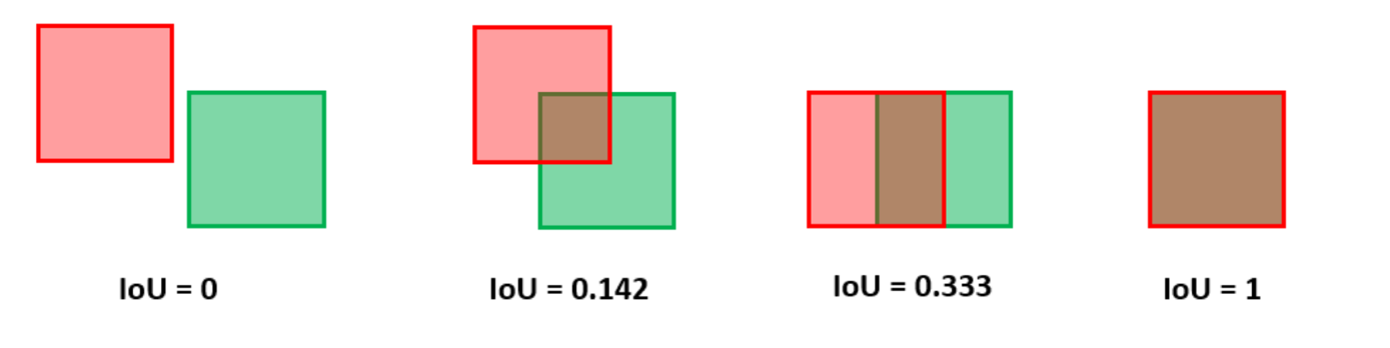
\includegraphics[width=\textwidth]{Iou.png}
        \caption{Schéma de l'Intersection over Union}
    \end{minipage}
\end{figure}

Pour qu'une détection soit considérée comme vraie, le taux de chevauchement entre la boîte d’annotation prédite et celle de la vérité terrain doit être supérieur à 0.5 (50\%). En-dessous de ce seuil de 0.5, la prédiction est considérée comme fausse. Ce seuil délibérément bas a été fixé dans les modalités d’évaluation des modèles lors des challenges PASCAL VOC, pour prendre en compte l’imprécision des boîtes d’annotation qui peut exister dans la vérité terrain \footcite[314]{everingham_pascal_2010}.
Cette métrique est indispensable pour calculer toutes les autres. Elle permet de déterminer : \\

\begin{itemize}
    \item Les vrais positifs (TP), c’est-à-dire un objet dont la classe et l’emplacement ont correctement été détectés.
    \item Les faux positifs (FP), c’est-à-dire une détection correcte de la classe d'un objet mais avec une localisation incorrecte, ou une attribution de classe erronée à un emplacement correspondant à un autre objet.
    \item Les faux négatifs (FN), c’est-à-dire un objet qui aurait dû être détecté mais ne l’a pas été.
\end{itemize}

Enfin, il existe les vrais négatifs (TN), correspondants aux objets qui ont été correctement non reconnus. Cette mesure est impossible à calculer et n’entre de fait pas dans les calculs des métriques.\\

L’IoU nous permet ainsi de calculer le Rappel et la Précision. C’est pourquoi il est important de déterminer le seuil en fonction des résultats attendus, qui influencera nécessairement le calcul de ces autres métriques.

\section{Le Rappel}

Le Rappel se définit par le nombre de vrais positifs (TP), classe et emplacement, au regard du nombre d’objets réellement présents, c’est-à-dire la somme des vrais positifs et des faux négatifs (FN). Ce score s’obtient grâce au calcul suivant :

\begin{center}
\begin{align*}
    R &= \frac{\text{Nombre de TP}}{\text{TP + FN}}
\end{align*}
\end{center}

Plus le score R s’approche de 1 plus le Rappel du modèle est important, c’est-à-dire qu’il détecte la totalité des documents pertinents, attribue les bonnes classes et les localise au bon endroit. En revanche, cela ne garantit pas sa précision. Un Rappel élevé peut également signifier la présence d’un grand nombre de faux positifs, noyant les données bien identifiées au milieu de fausses attributions, c’est-à-dire du bruit. 


\section[La Précision]{La Précision}

Les modèles étant, le plus souvent, entraînés pour analyser un grand nombre de données, un bruit trop important risque de limiter fortement l’exploration des données produites. Il faut donc s’assurer que la Précision du modèle est élevée. La Précision se définit par le nombre de documents correctement identifiés (TP) par rapport au nombre total d’objet détectés. Elle s’obtient donc par le rapport suivant :

\begin{center}
    \begin{align*}
    P &= \frac{\text{Nombre de TP}}{\text{TP + FP}}
    \end{align*}
\end{center}

Plus le score P s’approche de 1, moins le modèle produit de fausses attributions. Cela permet de réduire le bruit mais ne garantit pas que tous les objets à détecter l’ont été. Un modèle correctement entraîné devra présenter un Rappel et une Précision élevés. 

\newpage
\section[Le score F1]{Le score F1}

Le Score F1, appelé aussi \textit{Sørensen-Dice Coefficient}, permet de trouver le bon équilibre entre ces deux pondérations. Il s’obtient grâce à la moyenne harmonique des valeurs de Rappel et de Précision, grâce au calcul suivant :

\begin{center}
    \begin{align*}
    P &= 2 \frac{\text{recall .precision}}{\text{recall+precision}}
    \end{align*}
\end{center}

Un modèle parfait aurait un score F1 = 1, c’est-à-dire que la Précision et le Rappel du modèle seraient tous deux égaux à 1. A l’inverse, un déséquilibre important entre Rappel et Précision sera fortement pénalisé par cette métrique. Il s’agit donc, si l’on cherche l’équilibre entre la Précision et le Rappel, d’obtenir un score le plus proche de 1, afin de garantir que le modèle détecte correctement tous les objets. En combinant le Rappel et la Précision, le score F1 fournit une évaluation globale de la performance d'un modèle. \\

Ces métriques sont cruciales pour évaluer la qualité d'un modèle, en particulier dans des scénarios où les classes sont déséquilibrées ou lorsque les faux positifs et les faux négatifs ont des coûts différents.

\section[Le score de confiance]{Le score de confiance}

Cette métrique est automatiquement calculée par le modèle lors de la détection. Lorsque le modèle génère des prédictions de détection, chaque prédiction est accompagnée d'un score de confiance qui reflète à quel point le modèle estime que sa prédiction est précise. Plus le score de confiance est élevé, plus le modèle est sûr de la détection. Les prédictions avec des scores de confiance faibles indiquent que le modèle est peu sûr de sa détection. Dans les paramètres YOLO, un score de confiance inférieur à 0.25 ne donne pas lieu à une annotation \footnote{\url{https://docs.ultralytics.com/modes/predict\#inference-arguments}}. Il est possible de modifier ce paramètre, ce qui entraînera des conséquences sur la Précision et le Rappel. \\

\paragraph{Conclusion}Le score de confiance associé au Rappel, à la Précision et au score F1 permet de mieux cerner les ajustements à apporter au modèle pour qu’il puisse effectuer correctement les détections souhaitées. Il est tout aussi important d’évaluer le Rappel, la Précision et le score F1 de l’ensemble des classes d’annotations que pour chacune de ces classes. Ceci est particulièrement nécessaire lorsque les classes ne sont pas uniformément représentées au moment de l’entraînement ou si certaines classes sont plus complexes que d’autres \footcite[46]{hutchison_dataset_2006}.

\chapter{Analyse des résultats sur l’inférence des premiers modèles }

\section{Introduction}

Pour déterminer la robustesse des modèles entraînés nous avons évalué pour chaque modèle ses scores de Rappel, de Précision et F1 pour l’ensemble des classes, mais également pour chaque classe d’annotation. Chaque modèle a été évalué sur un jeu de données différent. Nous présenterons ici les résultats de ces premiers entraînements et les jeux de données sur lesquels ils ont été déployés. Chaque détection a généré un fichier ‘txt’, au nom de l’image, contenant les données suivantes : \\
\begin{itemize}
    \item Code de la classe,
    \item Coordonnées relatives de la boîte d’annotation (coordonnée x du centre de la boîte, coordonnée y du centre de la boîte, largeur de la boîte, hauteur de la boîte)
    \item Indice de confiance.
\end{itemize}

\paragraph{}Ces fichiers nous ont permis d’afficher les annotations dans \textit{Label Studio} et de corriger directement les mauvaises détections, générant ainsi de nouveaux fichiers ‘txt’, au nom de l’image, avec les données corrigées permettant de calculer les métriques d’évaluation des modèles \footnote{\url{https://github.com/Chaouabti/Memoire_TNAH_2023/blob/main/Training_model_workflow/4_Model_evaluation.ipynb}}. Nous avons fait le choix de calculer les métriques de l’ensemble des classes d’annotations et de chacune des classes pour proposer des stratégies afin d’améliorer les modèles et les rendre les plus précis possibles. Les résultats de chaque entraînement sont présentés sous forme de tableaux indiquant pour chaque classe : l’ensemble des données, le nombre de vrais positifs (TP), de faux positifs (FP) et de faux négatifs (FN) et les résultats de la précision, du rappel et du score F1.

\section{Résultats de l'entraînement \textit{Coat of Arms}}

Dans le cadre du jeu de données \textit{Coat of Arms}, nous avons entraîné le modèle avec le modèle large YOLOv8. Le \textit{dataset} étant suffisamment riche, nous avons conservé 10\% du \textit{dataset} comme jeu de données test sur lequel nous avons déployé le modèle. \\

\begin{table}[ht]
    \centering
    \begin{tabular}{|c|c|c|c|c|c|c|}
    \hline
    \textbf{Classe} & \textbf{TP} & \textbf{FP} & \textbf{FN} & \textbf{Rappel} & \textbf{Précision} & \textbf{Score F1} \\
    \hline
    timbre & 506 & 19 & 8 & 0.9844 & 0.9638 & 0.974 \\ 
    \hline
    coa & 1190 & 62 & 20 & 0.9835 & 0.9504 & 0.9667 \\ 
    \hline
    reverse-coa & 57 & 8 & 1 & 0.983 & 0.877 & 0.927 \\ 
    \hline
    stamp & 9 & 1 & 0 & 1 & 0.9 & 0.95 \\ 
    \hline
    banner-coa & 25 & 1 & 13 & 0.656 & 0.962 & 0.781 \\ 
    \hline
    pennant-coa & 3 & 2 & 1 & 0.75 & 0.6 & 0.67 \\ 
    \hline
    knight & 7 & 5 & 2 & 0.78 & 0.58 & 0.67 \\ 
    \hline
    clothing-coa & 10 & 10 & 3 & 0.77 & 0.5 & 0.61 \\ 
    \hline
    Total & 1807 & 108 & 48 & 0.9741 & 0.9436 & 0.9586 \\
    \hline
    \end{tabular}
    \caption{Résultats du premier entraînement \textit{Coat of Arms}}
\end{table}


Les résultats globaux de ce premier entraînement sont satisfaisants, malgré des disparités importantes. Les faux négatifs sont peu nombreux (ils représentent moins de 0,2\% des annotations) et concernent principalement les classes les moins représentées. Les faux positifs sont dus à trois raisons principales : \\
\begin{itemize}
    \item Détection d’armoiries fragmentaires, représentées dans les marges de l’image (généralement des armoiries peinte sur le folio suivant). Certaines ont été détectées par le modèle mais non annotées dans la vérité terrain.
    \item Détection (mais pas systématiquement) d'écussons représentés dans les armoiries : ceux-ci ont parfois été annotés mais pas systématiquement. Il sera donc nécessaire de nettoyer la vérité terrain et, éventuellement, de créer une nouvelle classe pour les armoiries avec écusson (coa-with-coa).
    \item Détection des reverse-coa confuse, en partie due à une annotation non homogène (un certain nombre de reverse-coa n’ont pas été annotés). Une rectification dans la vérité terrain permettrait d’affiner le modèle pour cette classe d’annotation.
\end{itemize}

\paragraph{}Les classes les moins représentées dans le jeu de données d’entraînement sont difficilement reconnues par le modèle et souvent confondues avec des éléments architecturaux. La classe ‘banner-coa’ est particulièrement mal reconnue, près d’un tiers des représentations n’a pas été correctement détecté. La classe ‘clothing-coa’ est mal détectée, avec autant de TP que de FP, montrant une grande confusion dans le modèle pour cette classe. Cela peut s’expliquer par la variabilité des formes et des motifs qui composent cette classe, allant de vêtements ornés d’armoiries aux tentures. De même, la classe ‘knight’ a été correctement détectée autant de fois qu’il y a eu de mauvaises détection et attributions.

\paragraph{Conclusion}Le jeu de données d’entraînement mérite d’être repensé et la vérité terrain réannotée.

\section{Résultats de l'entraînement Miniatures}

Nous avons entraîné avec le même jeu de données ‘Miniatures’ deux modèles avec YOLOv8, en utilisant pour le premier le poids pré-entraîné yolov8m.pt, et pour le second yolov8l.pt. La différence entre ces deux modèles est la taille et la qualité des scores : yolo8l.pt est plus lourd mais plus efficient que yolo8m.pt \footnote{\url{  https://docs.ultralytics.com/models/yolov8/\#overview }}. Nous avons gardé les mêmes hyperparamètres à savoir époques, batch, workers, taille de l’image. Pour évaluer la robustesse des deux modèles nous les avons déployés sur des manuscrits de livres d’heures issus de la liste des manuscrits d’HORAE. Les données d’entraînement étant également issues de livres d’heures, nous avons pris soin d’éliminer de nos analyses les images utilisées pour l’entraînement. Cela nous permet d’avoir une évaluation fiable dans un contexte naturel, avec un grand nombre de folios où aucune miniature n’est présente. A noter que toutes les images soumises à l’entraînement du modèle étaient annotées. Nous avons déployé le modèle entraîné avec yolo8m.pt sur les manuscrits suivants :

\begin{itemize}
    \item La Haye, Bibliothèque royale, ‘Heures de Simon de Varye’ (74 G 37 a),
    \item La Haye, Bibliothèque royale, ‘Heures trivulziano’ (KW 1900 A 009),
    \item Angers, Musée des Beaux-arts, ‘Heures à l'usage de Paris’ (2003.1.073),
    \item Angers, Bibliothèque municipale, ‘Heures à l’usage d’Angers’ (Ms. 2111),
    \item Arras, Bibliothèque municipale, ‘Sanctæ Crucis’ (CGM 751 / Ms 780)
\end{itemize}


\begin{table}[ht]
    \centering
    \begin{tabular}{|c|c|c|c|c|c|c|}
    \hline
    \textbf{Manuscrit} & \textbf{TP} & \textbf{FP} & \textbf{FN} & \textbf{Rappel} & \textbf{Précision} & \textbf{Score F1} \\
    \hline
    Heures de Simon de Varye & 36 & 4 & 6 & 0.889 & 0.842 & 0.865 \\ 
    \hline
    Heures trivulziano & 66 & 36 & 0 & 0.455 & 1 & 0.625 \\ 
    \hline
    Heures à l'usage de Paris & 19 & 3 & 0 & 0.842 & 1 & 0.914 \\ 
    \hline
    Heures à l’usage d’Angers & 25 & 2 & 0 & 0.92 & 1 & 0.958 \\ 
    \hline
    Sanctæ Crucis & 23 & 0 & 0 & 1 & 1 & 1 \\ 
    \hline
    \end{tabular}
    \caption{Résultats de l'entraînement Miniatures avec YOLOv7}
\end{table}

Les scores du modèle sur les différents manuscrits sont très hétérogènes. Les faux positifs sont principalement dus à la présence de majuscules ornées, en particulier dans le cas du manuscrit des \textit{Heures trivulziano}, dans lequel elles représentent 14 des 20 FP (70\%). Ce manuscrit est particulièrement intéressant pour réfléchir aux classes des miniatures :  le modèle a correctement détecté 14 majuscules historiées, soit autant que de majuscules ornées détectées. Dans le manuscrit des \textit{Heures de Simon de Varye}, tous les FN sont des miniatures présentes dans des médaillons marginaux.

Pour améliorer la précision, il sera peut-être intéressant d’introduire deux nouvelles classes : \\
\begin{itemize}
    \item Une pour les médaillons marginaux,
    \item Une pour les majuscules historiées afin de les différencier des majuscules ornées. 
\end{itemize}

\paragraph{}Le modèle entraîné avec yolo8l.pt a été déployé sur les mêmes manuscrits et les résultats sont beaucoup moins satisfaisants. Tous les folios du manuscrit des \textit{Heures trivulziano} ont fait l’objet d’une détection (654), avec parfois des détections qui se chevauchent. À la vue de ce constat, nous n’avons pas corrigé manuellement ces données et nous nous sommes concentrés sur le manuscrit des \textit{Heures de Simon de Varye} (74 G 37 a), dont les résultats sont représentatifs de la médiocrité du modèle. Sur les 220 folios, 111 ont fait l’objet de détection par le modèle.\\

\begin{table}[ht]
    \centering
    \begin{tabular}{|c|c|c|c|c|c|c|}
    \hline
    \textbf{Manuscrit} & \textbf{TP} & \textbf{FP} & \textbf{FN} & \textbf{Rappel} & \textbf{Précision} & \textbf{Score F1} \\
    \hline
    Heures de Simon de Varye & 43 & 99 & 11 & 0.796 & 0.303 & 0.439 \\ 
    \hline
    \end{tabular}
    \caption{Résultats de l'entraînement Miniatures avec YOLOv8}
\end{table}

\paragraph{}Les scores sont très insatisfaisants, avec une précision de 0.303. Plus de la moitié des folios présentent une détection, ce qui témoigne de l’incapacité du modèle à reconnaître correctement les miniatures. Les marges ornées de motifs floraux sont systématiquement détectées, voire font l’objet de multiples détections. Pourtant, le jeu de données d’entraînement présentaient des folios avec des miniatures annotées et des marges ornées de motifs non annotées. A l’inverse, les médaillons marginaux présentant des scènes historiées et devant être détectées ne l’ont pas été. Ces résultats témoignent d’une nécessité de spécifier davantage les types de miniatures, comme les médaillons marginaux et éventuellement les majuscules historiées. Il serait également pertinent d’augmenter significativement le jeu de données d’entraînement. \\

\paragraph{Conclusion}Au vu de ces résultats, il nous semble nécessaire d’augmenter le nombre de classes pour pouvoir détecter correctement les miniatures présentes dans les médaillons marginaux. Le choix du modèle a été déterminant sur les résultats, nous nous attarderons à proposer une nouvelle ontologie pour réentraîner un modèle avec yolo8l.pt.


\section{Résultats de l'entraînement \textit{Books in books}}

Le modèle ‘Books in books’ a été déployé sur 350 miniatures issues d’HORAE.


\begin{table}[ht]
    \centering
    \begin{tabular}{|c|c|c|c|c|c|c|}
    \hline
    \textbf{Classe} & \textbf{TP} & \textbf{FP} & \textbf{FN} & \textbf{Rappel} & \textbf{Précision} & \textbf{Score F1} \\
    \hline
    Codex & 330 & 42 & 11 & 0.968 & 0.887 & 0.926 \\ 
    \hline
    Banderole & 55 & 35 & 3 & 0.943 & 0.611 & 0.743 \\ 
    \hline
    Single-Sheet Document & 1 & 0 & 0 & 1 & 1 & 1 \\ 
    \hline
    Scroll & 25 & 17 & 2 & 0.926 & 0.596 & 0.725 \\ 
    \hline
    Total & 411 & 94 & 16 & 0.963 & 0.814 & 0.882 \\ 
    \hline
    \end{tabular}
    \caption{Résultats de l'entraînement \textit{Books in books}}
\end{table}

Les résultats de ce premier entraînement montrent que pour les différentes classes le Rappel est satisfaisant (plus de 0.9 pour chaque classe), contrairement à la Précision. Il n’est en revanche pas possible de tirer de conclusions sur les scores de la classe ‘Single-Sheet Document’, en raison d’un témoin unique dans le jeu d’inférence correctement détecté. Les scores de cette classe contrastent fortement avec ceux des autres classes, en étant bien supérieur mais non déterminants. Cet exemple témoigne parfaitement de la nécessité de calculer les métriques des différentes classes et de prendre en compte le nombre de témoin de chaque classe.

\newpage
\begin{figure}[ht]
    \centering
    \begin{minipage}[b]{0.45\textwidth}
        \centering
        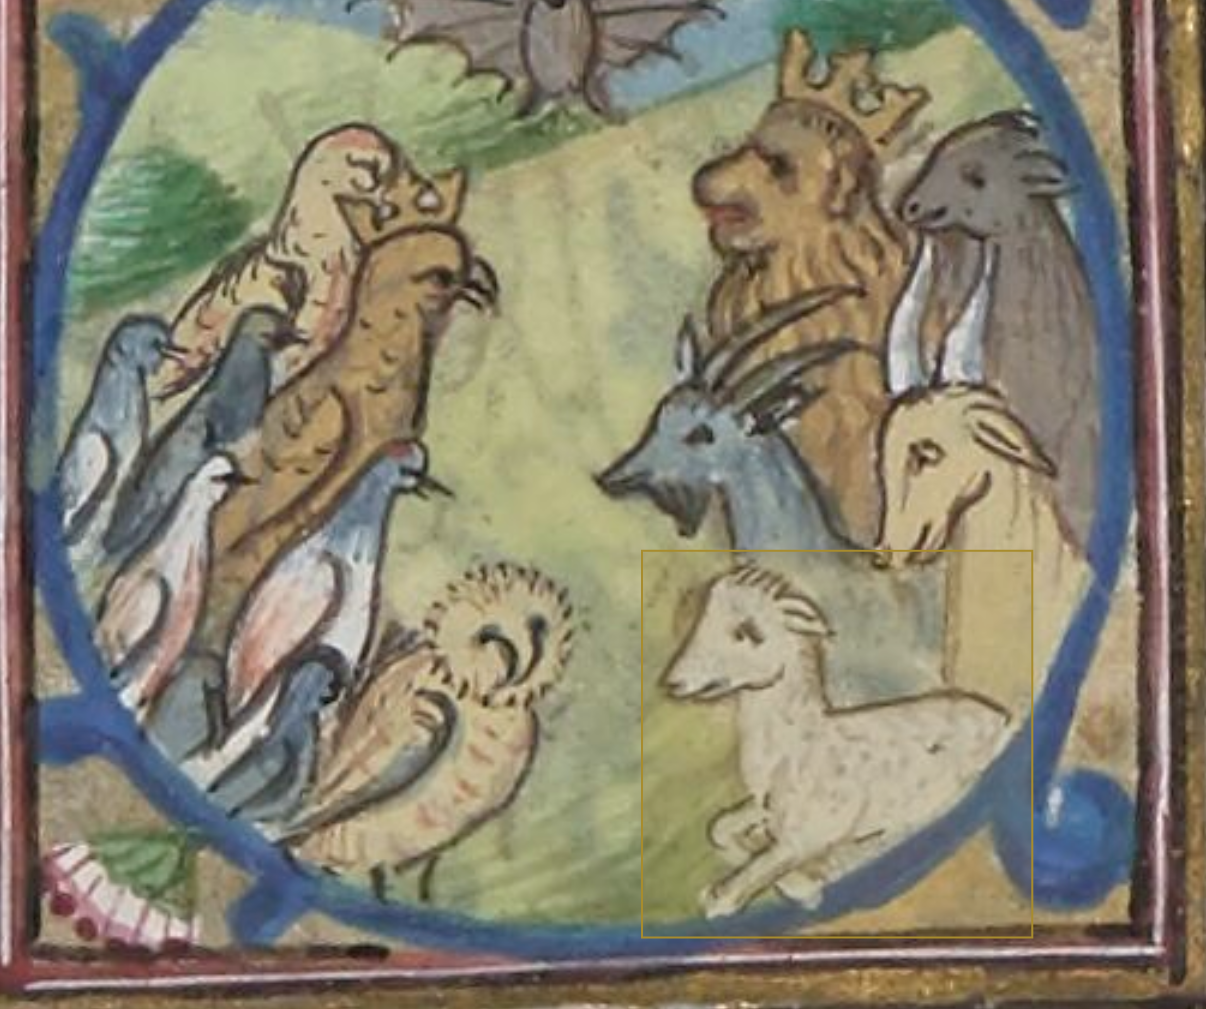
\includegraphics[width=\textwidth]{agneau_scroll.png}
        \caption{Un agneau identifié comme ‘scroll’ (\url{https://gallica.bnf.fr/iiif/ark:/12148/btv1b10527644s/f251/779,2169,507,511/full/0/default.jpg})}
    \end{minipage}
\end{figure}



Le nombre de faux positifs est très élevé dans les différentes classes, entraînant un mauvais score de Précision.  Les faux positifs de la classe ‘banderole’ sont particulièrement nombreux. Lors de la correction nous avons constaté que tout aplat blanc ou ocre clair est détectés comme ‘scroll’.  La majorité des faux positifs de la classe ‘banderole’ sont dus à une mauvaise détection des \textit{Titulus crucis} dans les scènes de crucifixions systématiquement étiqueté ‘banderole’. Les autres faux positifs sont dus à des doubles détections. \\

\begin{figure}[ht]
    \centering
    \begin{minipage}[b]{0.45\textwidth}
        \centering
        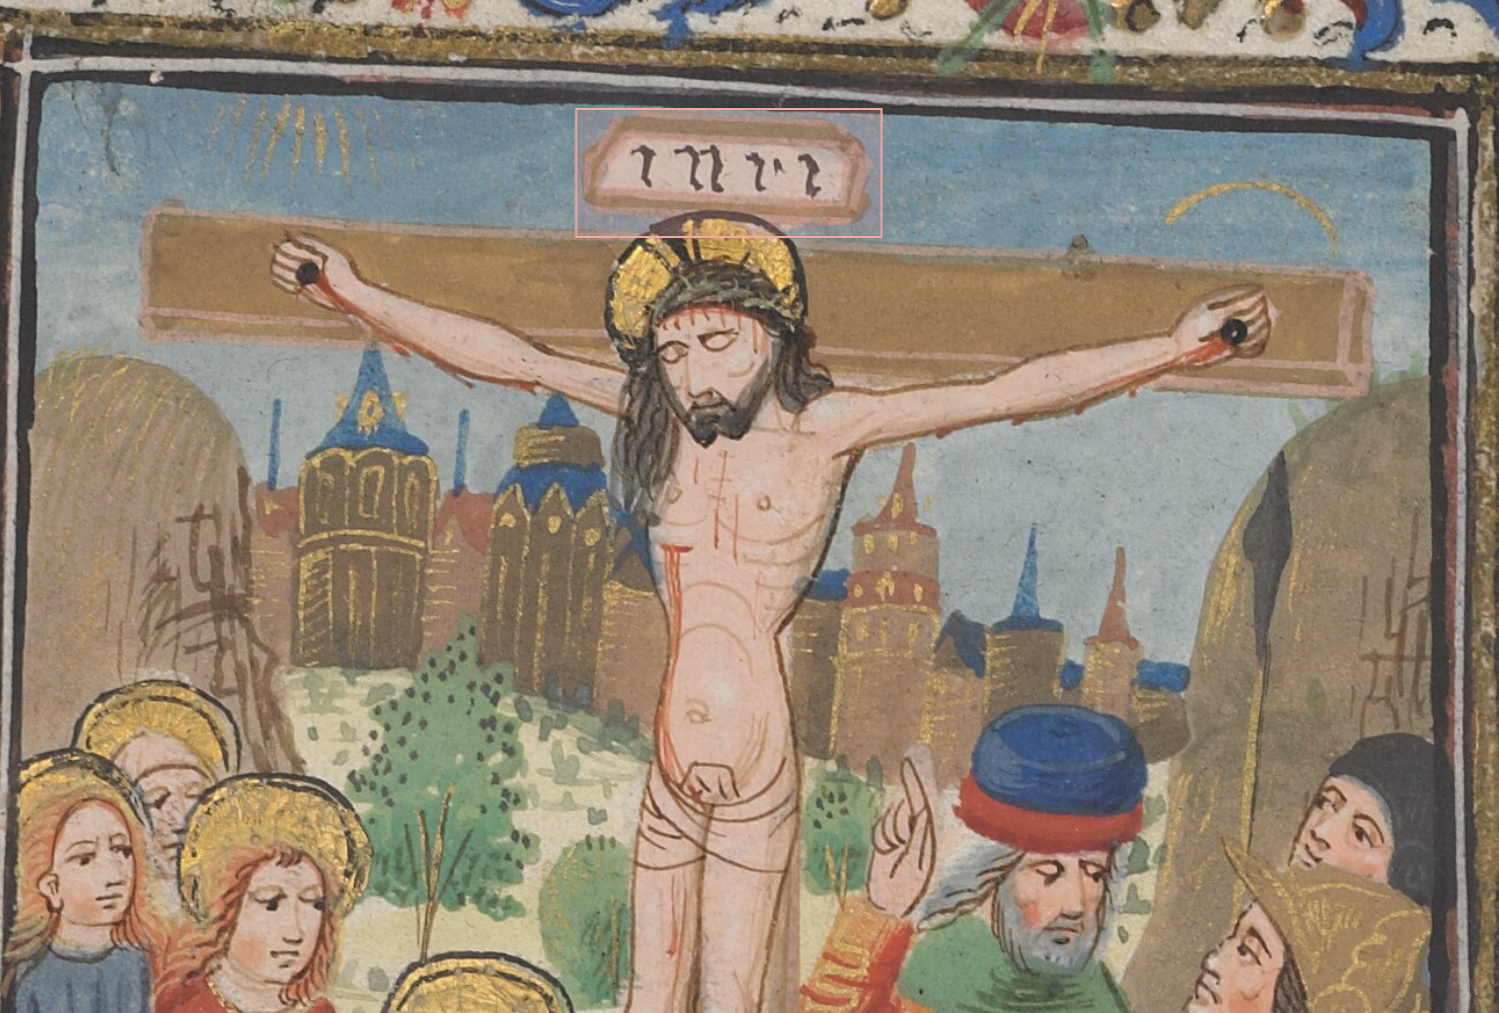
\includegraphics[width=\textwidth]{Titulus crucis.png}
        \caption{\textit{Titulus crucis détecté comme 'scroll'}}
    \end{minipage}
    \hfill
    \begin{minipage}[b]{0.45\textwidth}
        \centering
        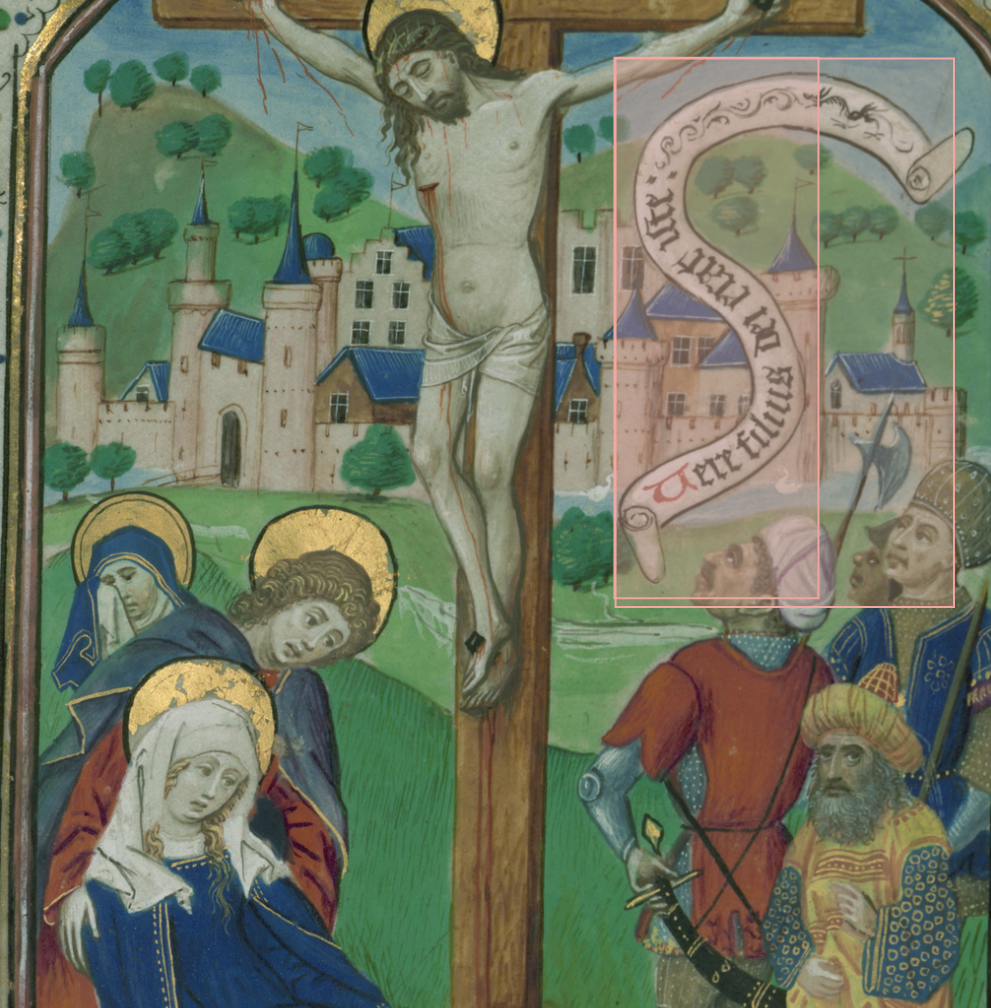
\includegraphics[width=\textwidth]{Double_Scroll.png}
        \caption{Détection multiple d'une même classe 'scroll'}
    \end{minipage}
\end{figure}


\newpage
Enfin, la classe ‘codex’ est celle avec le plus haut score de Rappel mais également celle pour laquelle aucun élément iconographique ne peut être identifié comme source de confusion ou de mauvaise détection. Les mains semblent être le motif iconographique le plus présent dans les fausses détections, ce qui est probablement lié à la nature même de la classe : de nombreux \textit{codices} du jeu d’entraînement sont représentés tenus à la main impliquant nécessairement la présence de ce motif spécifique dans les boîtes d’annotations. 

\begin{figure}[ht]
    \centering
    \begin{minipage}[b]{0.45\textwidth}
        \centering
        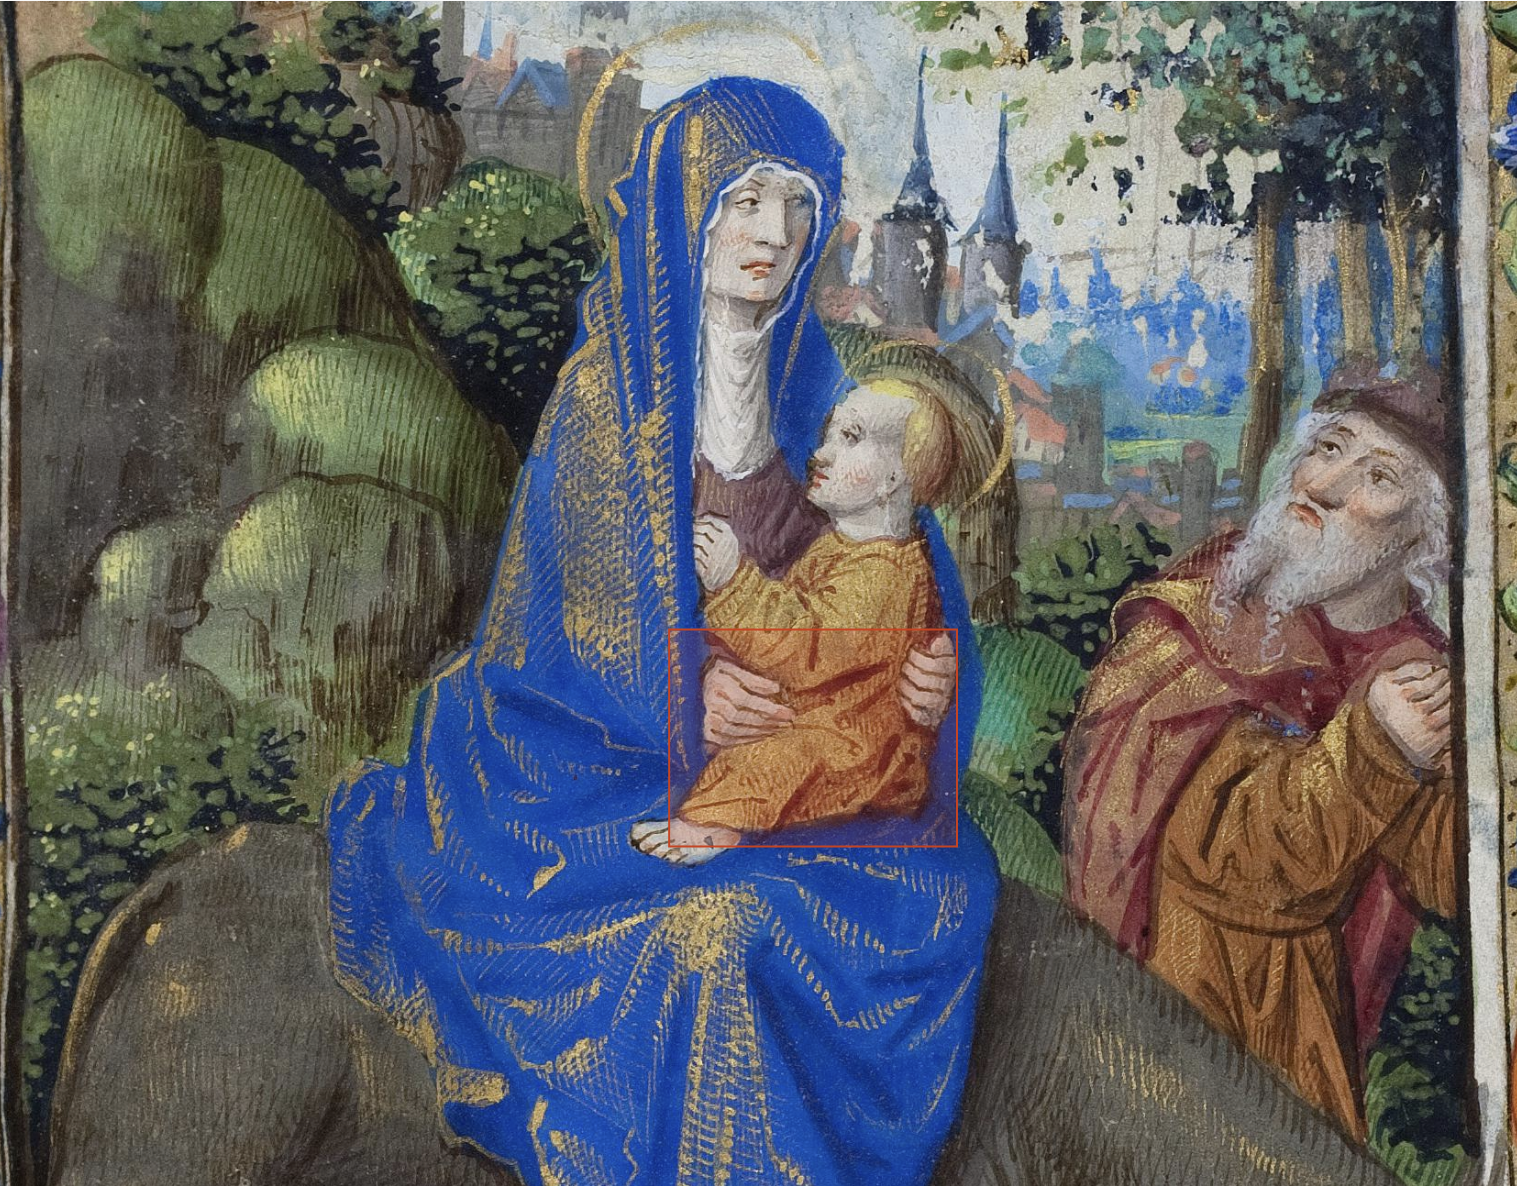
\includegraphics[width=\textwidth]{Codex_non.png}
        \caption{Exemple de mauvaise détection de la classe 'codex'}
    \end{minipage}
\end{figure}

\paragraph{Conclusion}Le Rappel du modèle est élevé contrairement à la précision, il ne semble donc pas nécessaire de modifier l’ontologie première. En revanche, le \textit{dataset } d’entraînement n’est pas suffisamment large et une augmentation des données, permettra certainement d’améliorer le score de précision du modèle. 


\section*{Conclusion}

L’évaluation de ces différents modèles témoigne des différents cas de figures qui peuvent survenir dans le cadre d’une analyse de données historiques par computer vision. Chacune des classes peut inclure des motifs conceptuellement similaires mais parfois très différents formellement. Cela se distingue particulièrement pour les miniatures qui peuvent se déployer dans des cadres rectangulaires, des majuscules ou des médaillons. L’annotation de ces données est complexifiée par les disparités stylistiques qui peuvent survenir entre deux manuscrits entraînant des erreurs dans la vérité terrain et influençant, de fait, l’apprentissage du modèle. Il est donc nécessaire, en fonction des différents cas et de la nature même des données, d’adapter une stratégie spécifique afin de répondre au mieux aux problématiques historiques au fondement même du développement des projets de computer vision. L’enjeu de l’utilisation de la \textit{computer vision} est à la fois de mettre en place des traitements automatisés des données mais aussi d’affiner notre regard sur le matériel d’étude. 

\chapter{Stratégies d’amélioration des modèles}

\section{Introduction}

Les résultats des premiers entraînements témoignent des problèmes de modélisation. Ils témoignent également de la nécessité de repenser la pertinence des choix et des démarches afin d’affiner l’approche historique et de développer des stratégies d’amélioration des modèles en fonction des premiers résultats et des besoins de la recherche. Les résultats des premiers entraînements montre que les modèles peuvent être améliorés selon deux grands schémas :

\begin{itemize}
    \item Corriger le jeu de données, en éliminant les biais induits par une nouvelle annotation, une augmentation des données d’entraînement ou une répartition plus maîtrisée des classes.
    \item Repenser la modélisation de base, la répartition des classes, voire adopter une nouvelle approche afin de redéfinir une ontologie plus à même de répondre à la problématique d’origine. 
\end{itemize}

\paragraph{}Dans ce cadre nous avons essayé différentes approches que nous détaillons ici en présentant les résultats obtenus. Les différents modèles entraînés sont présentés dans l’Annexe 2. Nous signalerons ici les modèles avec le nom utilisé pour les nouveaux entraînements, qui correspond également au nom du modèle tel qu’il est renseigné dans les annexes. 

\newpage
\section{Repenser le \textit{dataset}}
\subsection{Correction de la vérité terrain}

En corrigeant manuellement les données et en utilisant des données annotées, mais non utilisées pour l’entraînement, nous avons pu constater que la détection de motifs ne correspondant pas à leur boîte d’annotation, faux positifs ou négatifs, pouvait être due à une mauvaise annotation de la vérité terrain. \\

Dans le jeu de données Miniatures, les mauvaises annotations de la vérité terrain ont été induites par une inadéquation entre la taille de l’image telle qu’elle est déclarée dans le manifeste et la taille réelle de l’image accessible via l’URL. Cela a eu pour conséquence de placer les boîtes d’annotations aux mauvais endroits. La position des boîtes d'annotation dans les marges des manuscrits explique, en partie, la présence de ces mêmes marges ornées dans les détection du modèle. Par ailleurs, l’annotation automatisée de ce corpus a entraîné l'absence d'annotation pour toutes les miniatures au sein de certains folios. Nous avons donc dans un premier temps réannoté correctement la vérité terrain.


\begin{figure}[ht]
    \centering
    \begin{minipage}[b]{0.45\textwidth}
        \centering
        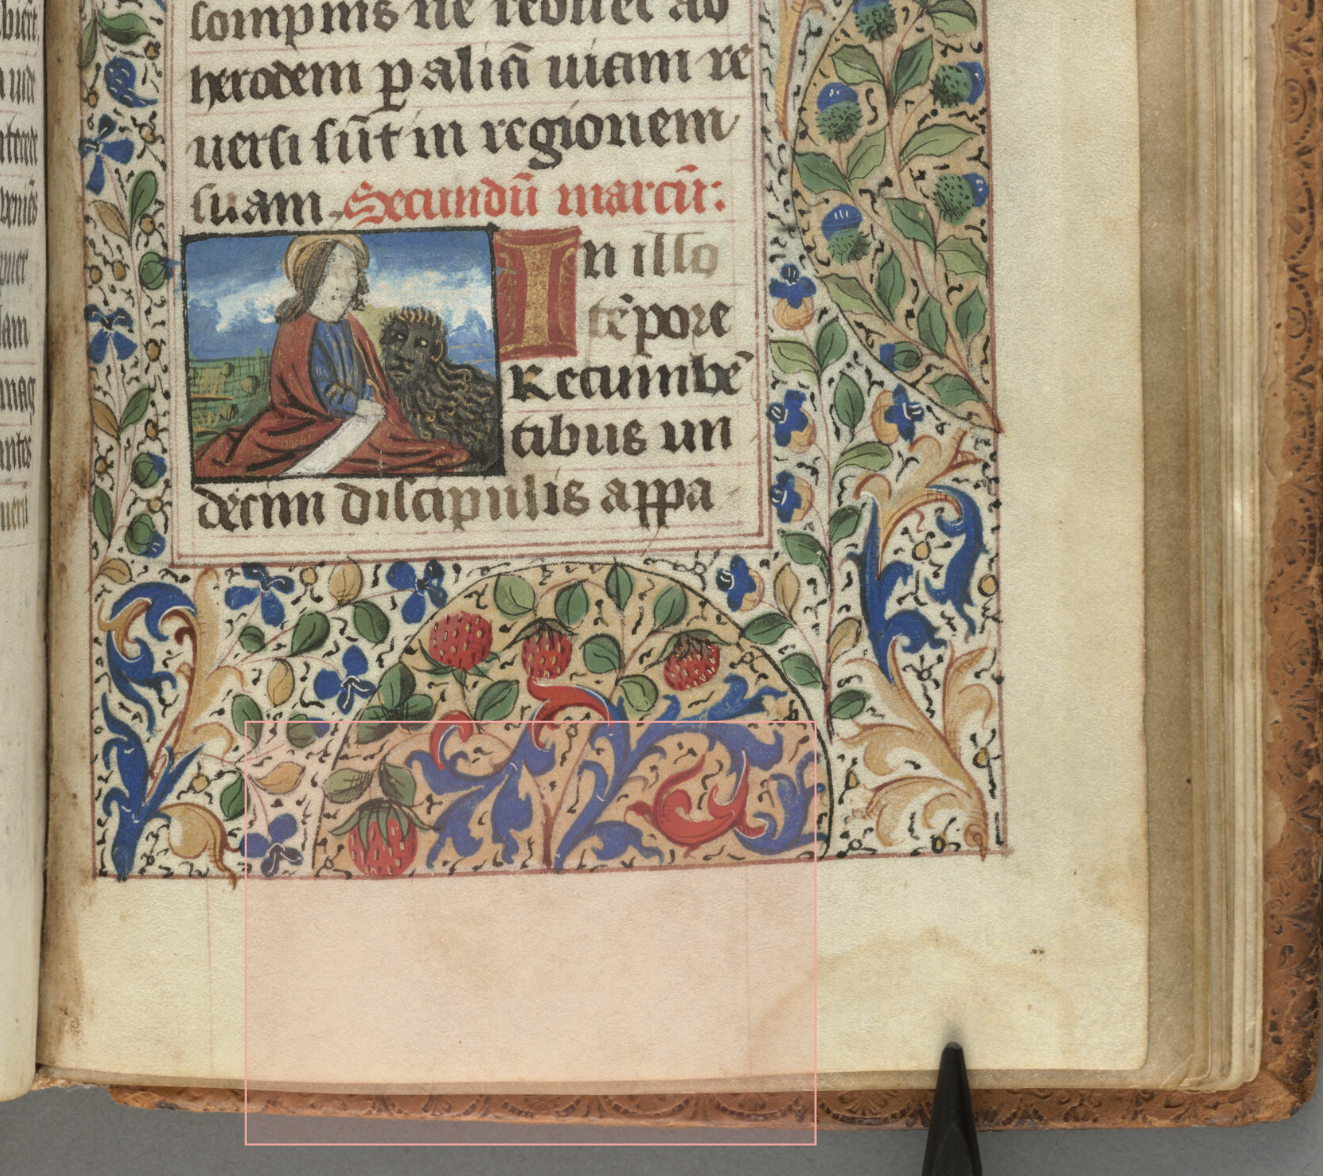
\includegraphics[width=\textwidth]{PB_Image.png}
    \end{minipage}
    \hfill
    \begin{minipage}[b]{0.45\textwidth}
        \centering
        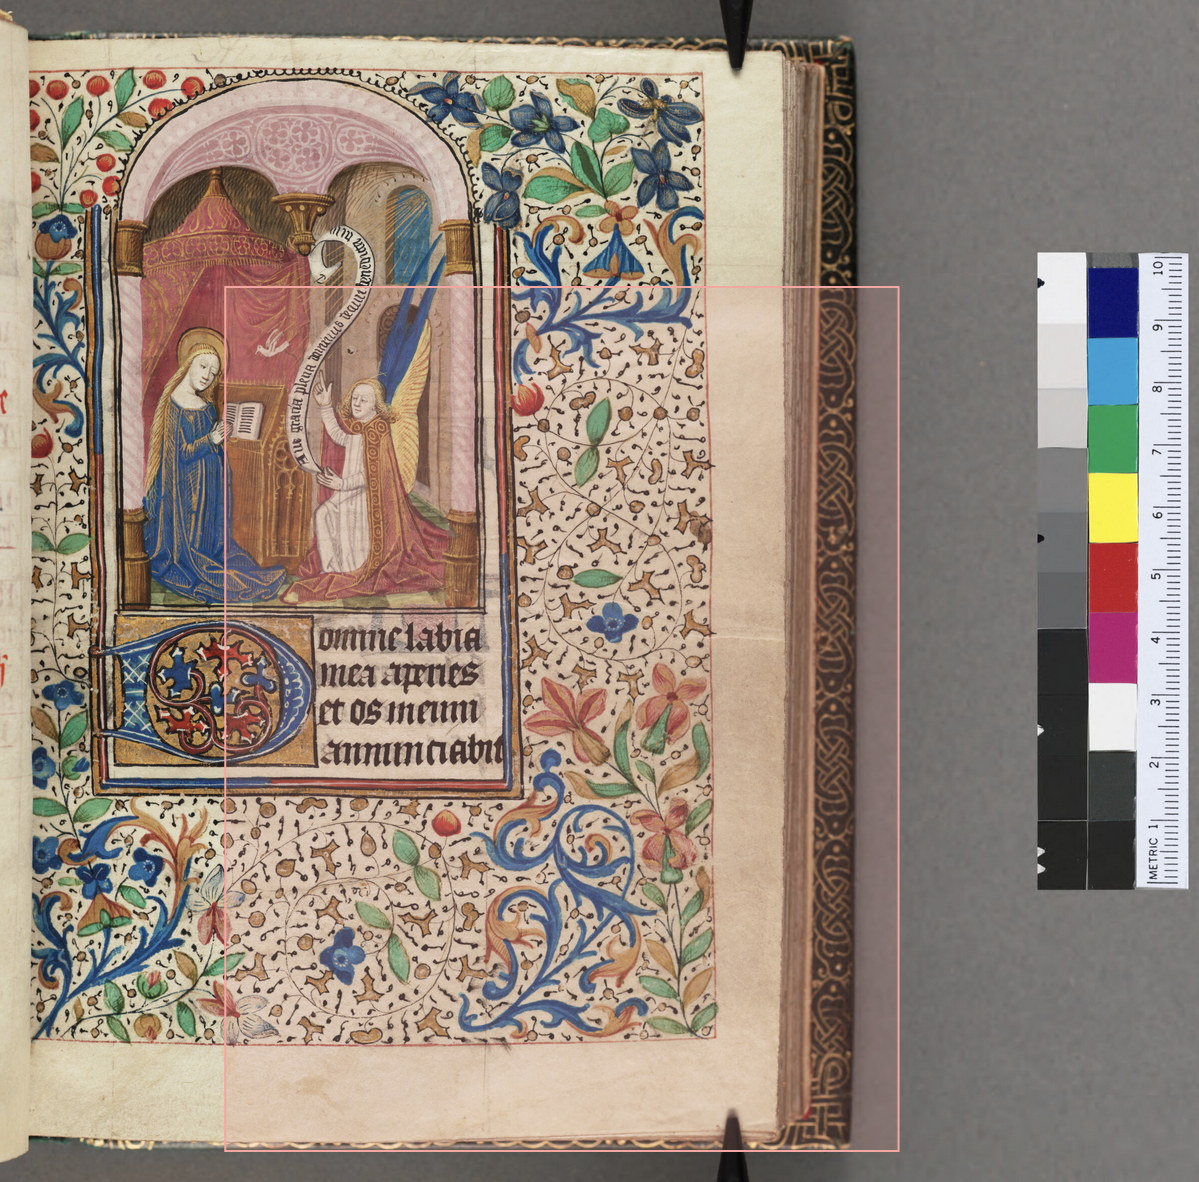
\includegraphics[width=\textwidth]{PB_IMAG2.png}
    \end{minipage}
    \caption{Boîtes d'annotation mal détectée en raison des problèmes de la vérité terrain }
\end{figure}

Dans le jeu de données \textit{Coat of Arms} nous avons constaté un certain nombre de données mal annotées pouvant découlées d’une ontologie trop complexe ou pas assez spécifique, laissant place à l’ambiguïté. Ce risque est d’autant plus accru dans le cadre des annotations du jeu de données \textit{Coat of Arms} où différentes personnes ont la charge de l’annotation. Le jeu de données utilisé était suffisamment étendu pour le modèle soit entraîné correctement. Néanmoins pour s’assurer d’entraîner un modèle le plus robuste possible il est nécessaire de corriger la vérité terrain.  

\paragraph{Conclusion}La qualité des données et de leur annotation constituent la pierre angulaire de tout projet en \textit{computer vision}. Nous constatons bien qu'un \textit{dataset} mal préparé entraîne des faiblesses dans le modèles entraîné, là où un \textit{dataset} parfaitement préparé constitue un atout majeur pour l’entraînement des modèles permettant de se concentrer sur des stratégies plus efficaces. 

\subsection{Augmentation des données}

La taille du dataset d’entraînement et la bonne représentation des différentes classes d’annotations sont deux éléments déterminants pour produire des modèles robustes. Un ensemble de données annotées plus important serait donc nécessaire pour améliorer les performances et la capacité de généralisation de notre modèle \footcite{aouinti_illumination_2022}.
Si l’annotation est une tâche importante mais chronophage, l’utilisation de données issues de bonnes prédictions ou de prédictions corrigées est une stratégie facile à mettre en en place. Cela permet d’utiliser l’ensemble du jeu de données pour l’entraînement, de tester le modèle sur des données neuves, d'augmenter le \textit{dataset }et d'évaluer les modèles grâce aux corrections. \\

Ainsi, pour améliorer le modèle \textit{Books in books} nous avons décidé d’augmenter le \textit{dataset} pour améliorer sa Précision. Pour ce faire nous avons ajouté les données corrigées détectées avec le modèle sur les miniatures issues d’HORAE. Cela nous a permis d’augmenter le jeu de données de 350 nouvelles miniatures. Nous avons déployé ce nouveau modèle (Books\_in\_books\_new\_data) sur des miniatures issues de livre d’heures. Les résultats de ce deuxième entraînement sont les suivants :\\


\begin{table}[ht]
    \centering
    \begin{tabular}{|c|c|c|c|c|c|c|}
    \hline
    \textbf{Classe} & \textbf{TP} & \textbf{FP} & \textbf{FN} & \textbf{Rappel} & \textbf{Précision} & \textbf{Score F1} \\
    \hline
    Codex & 330 & 42 & 11 & 0.968 & 0.887 & 0.926 \\ 
    \hline
    Banderole & 55 & 35 & 3 & 0.943 & 0.611 & 0.743 \\ 
    \hline
    Single-Sheet Document & 1 & 0 & 0 & 1 & 1 & 1 \\ 
    \hline
    Scroll & 25 & 17 & 2 & 0.926 & 0.596 & 0.725 \\ 
    \hline
    Total & 411 & 94 & 16 & 0.963 & 0.814 & 0.882 \\ 
    \hline
    \end{tabular}
    \vspace{0.5cm}  % Ajout d'un espace vertical
    \caption{Résultats de l'entraînement \textit{Books in books} avec ajout de nouvelles données}
\end{table}

\paragraph{}
Les résultats globaux sont étonnament moins bon que pour le premier entraînement. Le Rappel et le score F1 ont légèrement baissé mais la précision a augmenté. Pour les classes ‘codex’ et ‘scroll’ toutes les métriques sont meilleures. Pour la classe ‘banderole’ le Rappel est meilleur, en partie grâce l’absence de \textit{titulus crucis}, dont un seul a été détecté comme ‘banderole’. En revanche, la classe ‘single- sheet document’ n’a pas été détectée une seule fois.  Bien que nous ne puissions garantir qu’aucun objet du jeu de test ne corresponde à la classe d’annotation et celle-ci a systématiquement été confondue avec la classe ‘scroll’ dont elle se rapproche fortement d’un point de vue de formel. Cette classe étant par ailleurs peu présente, il serait judicieux de fusionner ‘single-sheet document’ et ‘scroll’ afin de limiter le classes trop proches et les faux positifs. La vérité terrain et l’ontologie apparaissent bien maîtrisées et un nombre croissant de données ajoutées au modèle participera certainement à augmenter sa robustesse. 

\paragraph{Conclusion}Dans ce cas précis, où la vérité terrain est bien annotée et l’ontologie maîtrisée, il serait plus favorable de \textit{fine tuner} le modèle en n’entraînant que la dernière couche plutôt que de réentraîner un nouveau modèle depuis les poids de YOLOv8, plus génériques.

\subsection{Une approche plus maîtrisée : vers l’isocardinalité }

Dans les différents jeux de données que nous avons envisagés, force est de constater une répartition inégale des classes d’annotations du fait même de la nature des données : une étude sur les armoireries intégrant un nombre important d’armoriaux implique naturellement une sur-représentation des classes ‘coa’ et ‘timbre’. Ces deux classes constituent  la quasi totalité du programme iconographique de ces manuscrits. De même, les miniatures dans les livres d’heures sont plus fréquemment représentées dans des cadres rectangulaire, parfois en pleine page, que dans des médaillons marginaux ou  des majuscules historiées. Ces répartition hétérogènes témoignent d’une représentation naturelle des données.  Se pose donc la question d’aller vers une représentation équilibrée des classes d’annotations, qui fausse dans le même temps la représentativité d’apparition des différentes classes. En augmentant artificiellement les données des classes sous-représentées, cela peut-il avoir un impact sur le modèle qui sera plus à même de détecter ces classes peu représentées, tout en entraînant un nombre important de faux postifs pour ces mêmes classe ? \\

La structure internes du jeu de données \textit{Coat of Arms} a rendu impossible la création d’un dataset avec une représentativité équivalente des différentes classes d’annotation. La classe 'coa' est toujours sur-représentée puisqu'il n'existe pas ou peu d'exemple d'images annotées avec la classe 'banner-coa' mais sans ‘coa’. Il était également exclu de supprimer des annotations pour ne pas impacter la qualité de l'entraînement des modèles qui auraient eu une vérité terrain non homogène avec certains objets ‘coa’ annotés et d'autres non.

\begin{table}[ht]
    \centering
    \begin{tabular}{|c|c|c|c|c|c|c|}
    \hline
    \textbf{Classe} & \textbf{TP} & \textbf{FP} & \textbf{FN} & \textbf{Rappel} & \textbf{Précision} & \textbf{Score F1} \\
    \hline
    timbre & 4010 & 290 & 292 & 0.9321 & 0.9326 & 0.93234 \\ 
    \hline
    coa & 9098 & 991 & 721 & 0.9266 & 0.9018 & 0.91 \\ 
    \hline
    reverse-coa & 405 & 101 & 81 & 0.8333 & 0.8004 & 0.8165 \\ 
    \hline
    stamp & 0 & 0 & 0 & 0 & 0 & 0 \\ 
    \hline
    banner-coa & 1 & 0 & 0 & 1 & 1 & 1 \\ 
    \hline
    pennant-coa & 0 & 0 & 0 & 0 & 0 & 0 \\ 
    \hline
    knight & 0 & 0 & 0 & 0 & 0 & 0 \\ 
    \hline
    clothing-coa & 1 & 0 & 0 & 1 & 1 & 1 \\ 
    \hline
    Total & 13515 & 1382 & 1094 & 0.92511 & 0.90723 & 0.91608 \\
    \hline
    \end{tabular}
    \vspace{0.5cm}  % Ajout d'un espace vertical
    \caption{Résultat de l'entraînement \textit{Coat of Arms} avec des données équilibrées}
\end{table}

\paragraph{}Dans l'ensemble, cet entraînement, fait avec un nombre plus restreint d'images, a montré des performances moyennes généralement plus basses mais une meilleure qualité de détection des classes sous-représentées. Dans ce cadre, une stratégie d'amélioration serait d'augmenter le \textit{dataset} en conservant au maximum un écart modéré entre la représentation des différentes classes d'annotations. Le modèle a été déployé sur les images d’entraînement du premier modèle \textit{Coat of Arms} qui n’ont pas servi à l’entraînement du modèle. Le nombre important d’annotation montre ici la nécessité de ne déployer que des modèles avec de très bonnes métriques : s’il est aisé de corriger manuellement une centaine d’annotation, l’exercice devient beaucoup plus fastidieux quand le nombre de FP et FN dépasse le millier. Il est donc nécessaire de toujours penser l’amélioration des modèles en fonction de leur utilité et de la marge d’erreur qu'il est possible d’accorder à de projet de traitement massif de données.  \\

\paragraph{Conclusion} Si les propriétés des objets de l'ensemble de données, telles que la taille et l'emplacement dans l'image, peuvent être considérées comme représentatives dans leur ensemble, il n'en va pas de même pour la fréquence d'apparition de chaque classe d'objets. Une répartition non naturelle mais mieux maîtrisée des données permet un meilleur apprentissage. 

\newpage
\section{Repenser la modélisation}

Si le jeu de données est bien maîtrisé, cohérent et les annotations rigoureuses, des résultats non satisfaisants peuvent témoigner d’une ontologie mal conçue qu’il est donc nécessaire de réadapter.

\subsection{Fusionner ou supprimer des classes}

Nous avons constaté qu'une meilleure répartition des annotations par classes permet d’obtenir de meilleure détections de ces mêmes classes. Dans le même nous avons constater que leur faible représentativité était en partie due à leur fréquence naturelle d’apparition dans les manuscrits dont sont issues les données d’entraînement. Il apparaît donc qu'il faille se questionner sur la présence même de la multiplicité de ces classes. Il a donc été envisagé pour le jeu de données \textit{Coat of Arms} de fusionner les classes les moins représentées en une seule nommée ‘non-shield-coa’. Cette classe recouvre ainsi toutes les classes avec armoiries mais non représentées sur des écus ou boucliers.

\begin{table}[ht]
    \centering
    \begin{tabular}{|c|c|c|c|c|c|c|}
    \hline
    \textbf{Classe} & \textbf{TP} & \textbf{FP} & \textbf{FN} & \textbf{Rappel} & \textbf{Précision} & \textbf{Score F1} \\
    \hline
    timbre & 502 & 222 & 5 & 0.99 & 0.958 & 0.974 \\ 
    \hline
    coa & 1182 & 58 & 19 & 0.984 & 0.953 & 0.968 \\ 
    \hline
    reverse-coa & 58 & 6 & 1 & 0.98 & 0.91 & 0.94 \\ 
    \hline
    non-shield-coa & 75 & 17 & 14 & 0.84 & 0.82 & 0.83 \\ 
    \hline
    Total & 1817 & 103 & 39 & 0.9789 & 0.9464 & 0.9624 \\
    \hline
    \end{tabular}
    \vspace{0.5cm}  % Ajout d'un espace vertical
    \caption{Résultats d'entraînement \textit{Coat of Arms} avec fusion des classes ‘non-shield-coa’}
\end{table}


\paragraph{}Si les résultats sont satisfaisants pour les trois classes principales que sont ‘coa’, ‘timbre’ et ‘reverse-coa’, ils chutent significativement pour la classe ‘non-shield-coa’.  Cette classe fourre-tout pose la question de la pertinence de regrouper en une seule classe une pluralité de motifs aux formes et aux fonctions bien distinctes. Par ailleurs, le jeu de test présente des données similaires à celles de l’entraînement ce qui ne garantit pas la robustesse du modèle sur des données héraldiques d’une nature différente, notamment dans les miniatures ou scènes historiées où les motifs sont plus complexes à analyser. \\

\paragraph{Conclusion} L’objectif du projet \textit{Digital Heraldry }étant d’identifier de manière massive des données héraldiques pouvant se trouver dans un grand nombre de manuscrits d’époques et de types différents, il semble pertinent d’augmenter la variété des données d’entraînement et de repenser une ontologie plus stricte et permettant d’accéder aux objectifs à l’origine même du projet. 

\subsection{Augmenter les classes}

Nous avons constaté après analyse des résultats de l’entraînement du modèle Miniatures, une confusion dans la détection des miniatures, de mauvaises attributions de classe à des majuscules ornées et la non-détection des médaillons marginaux. Nous proposons donc d’affiner l’ontologie en ajoutant deux nouvelles classes d’annotations : \\
\begin{itemize}
    \item ‘historiated\_initiale’ pour les initiales généralement plus grandes dont la décoration contient un élément iconographique et représente une scène ou un personnage \footcite{boillet_horae_2020}.
    \item ‘Marginal medallion’ pour les miniatures dans les marges, le plus souvent dans des cadres ronds, représentant le plus souvent des portraits (de saints) ou une représentation des travaux des champs. 
\end{itemize}

\paragraph{}
Ce qui peut apparaître comme une multiplication des classes d’annotation permet en réalité de limiter les faux négatifs et faux positifs. C’est la démarche qui a sous-tendue la création de la classe ‘reverse coa’ dans l’ontologie \textit{Coat of Arms}.  En distinguant les ‘coa’ des ‘reverse coa’, l’information fournie nous apprend qu’il n’y a pas à proprement parler de motifs héraldiques à rechercher dans le folio mais qu’il s’agit d’un effet de transparence, limitant ainsi le nombre de faux positifs qui viendrait fausser les résultats de la classe ‘coa’ en baissant sa Précision. Cette amplification des classes dans l’ontologie est une technique efficace mais qui augmente également le risque d’erreur : plus il y a de classes plus le risque de mauvaises annotations s’accroît. Il est nécessaire de toujours se poser la question de la pertinence de la création de classes spécifiques et de leurs définitions. La classe ‘historiated\_initiale’ pourra ainsi limiter le nombre de fausses détections d’initiales ornées, c’est-à-dire décorées d'éléments purement ornementaux (végétaux ou géométriques) et non iconographiques. \\

Nous avons donc entraîné un nouveau modèle Miniatures incluant les deux nouvelles classes d'annotation. Pour comparer les résultats, nous avons déployé ce nouveau modèle sur le même manuscrit que le modèle précédent : La Haye, Bibliothèque royale, \textit{Heures de Simon de Varye} (74 G 37 a). 

\begin{table}[ht]
    \centering
    \begin{tabular}{|c|c|c|c|c|c|c|}
    \hline
    \textbf{Classe} & \textbf{TP} & \textbf{FP} & \textbf{FN} & \textbf{Rappel} & \textbf{Précision} & \textbf{Score F1} \\
    \hline
    Miniature & 21 & 122 & 0 & 1 & 0.15 & 0.26 \\ 
    \hline
    Marginal medallion & 17 & 2 & 0 & 1 & 0.89 & 0.94 \\ 
    \hline
    Historiate initial & 0 & 0 & 0 & 0 & 0 & 0 \\ 
    \hline
    Total & 38 & 124 & 0 & 1 & 0.235 & 0.38 \\
    \hline
    \end{tabular}
    \vspace{0.5cm}  % Ajout d'un espace vertical
    \caption{Résultats entraînement \textit{Books in books} avec nouvelles classes sur les \textit{Heures de Simon de Varye}}
\end{table}

\paragraph{}
Nous constatons que les médaillons marginaux non reconnus avec le modèle précédent sont ici bien détectés au détriment de la classe ‘miniature’ dont le Rappel est bon mais la Précision extrêmement basse. Le constat est le même sur le manuscrit des \textit{Heures trivulziano}.  \\

\begin{table}[ht]
    \centering
    \begin{tabular}{|c|c|c|c|c|c|c|}
    \hline
    \textbf{Classe} & \textbf{TP} & \textbf{FP} & \textbf{FN} & \textbf{Rappel} & \textbf{Précision} & \textbf{Score F1} \\
    \hline
    Miniature & 32 & 43 & 0 & 1 & 0.43 & 0.6 \\ 
    \hline
    Marginal medallion & 1 & 6 & 0 & 1 & 0.15 & 0.25 \\ 
    \hline
    Historiate initial & 8 & 6 & 7 & 0.5 & 0.6 & 0.6 \\ 
    \hline
    Total & 41 & 55 & 7 & 0.85 & 0.427 & 0.569 \\
    \hline
    \end{tabular}
    \vspace{0.5cm}  % Ajout d'un espace vertical
    \caption{Résultats entraînement \textit{Books in books} avec nouvelles classes sur les \textit{Heures trivulziano}}
\end{table}

\paragraph{}Les majuscules historiées sont mal détectées et font parfois l’objet d’une double détection, ‘historiate initial’ et ‘miniature’. Par ailleurs, il y a une grande confusion entre les classes ‘historiate initial’ et ‘marginal medallion’. Enfin, cette classe ‘historiate initial’ initialement créée pour éviter les confusions entre miniature et majuscule ornée, ne semble pas avoir une véritable incidence sur les faux positifs que sont majuscules ornées. 

\paragraph{Conclusion}Au vu de ces résultats peu concluants, il importera d’augmenter le jeu de données, voire de repenser la modélisation ontologique. 

\subsection{Repenser la modélisation ontologique}

Dans l’ontologie \textit{Coat of Arms}, les classes actuelles combinent deux approches différentes : les classes pour la détection de formes (coa, timbre, stamp, banner-coa, pennant-coa et reverse-coa) et celles pour la détection de fonds. Les classes ‘clothing-coa’, ‘structure-coa’ et ‘non-shield-coa’ ne permettent pas rechercher des éléments formellement semblables mais plutôt des éléments dont la fonction est similaire. Les ‘clothing coa’ peuvent aussi bien être des armures que des manteaux royaux ou des parures de chevaux. De même, ‘structure-coa’ intègre, par exemple, les tentures comme les dais. Il apparaît comme nécessaire de distinguer ces deux tâches, fortement imbriquées d’un point de vue historique, mais très éloignées dans le cadre d’une recherche par computer vision. \\

Il sera donc judicieux d’entraîner un nouveau modèle en supprimant les classes d’annotations qui ne permettent pas de détecter une forme mais des motifs héraldiques. Nous pourrons ainsi intégrer de nouvelles classes permettant de détecter les ornements extérieurs aux écus (couronne, collier) et une classe pour les éléments proto-héraldiques (XIIe siècle) en raison d’une forme de bouclier différente de celles des siècles suivants. Dans cette nouvelle approche il sera également nécessaire de repenser le jeu de données en incluant d’avantage de miniatures pour multiplier les formes et contextes dans lesquels se retrouvent les boucliers, fanions, etc. La détection des boucliers dans les scènes complexes, notamment les scènes de batailles où les boîtes d’annotations se superposent et où les angles des boucliers sont multiples, n’est pas suffisamment efficace. Les manuscrits du cycle arthurien constitueraient à cet effet un jeu de données intéressant en raison de la présence fréquente de scènes de batailles contenues dans des miniatures où les chevaliers en armures s'affrontent en offrant des représentation de boucliers sous différents angles. \\

Cette nouvelle approche se déroulerait en deux temps : un premier où un modèle est entrainé pour détecter les différentes formes classiques sur lesquelles peuvent se déployer les motifs héraldiques et dans un deuxième temps rechercher les motifs héraldiques à proprement parler. L’idée étant de récupérer les objets sur lesquels se retrouvent les éléments héraldiques (boucliers, fanions, etc.) afin d’extraire les formes, puis de repasser ces nouvelles données dans un autre modèle qui permettra de retrouver les éléments héraldiques dans ces formes classiques.  \\

\newpage
\section{Repenser l'entraînement}

Si les données, leurs annotations et leur volume jouent un rôle considérable dans l’entraînement de modèle robuste, le choix de l’architecture et les poids d’entraînement sont tout aussi importants. Tous les entraînements que nous avons réalisés ont été repris systématiquement depuis le début en utilisant les poids génériques de YOLOv8. Cependant, lorsque que de nouvelles données sont prêtes à être intégrées dans le \textit{dataset} d'entraînement, il existe deux approches courantes : le réentraînement complet du modèle depuis le début et le \textit{fine-tuning} en utilisant les poids préalablement entraînés.

\subsection{Réentraînement complet de nouveaux modèles}

La rapidité de YOLOv8 et ses performances nous autorise à réentraîner intégralement un modèle rapidement. L’intérêt de réentraîner un modèle \textit{from scracth} est de garantir que l’ensemble des données utilisées ont été corrigées, que les classes d’annotation sont bien définies et que les erreurs qui ont pu être apprises dans les entraînements précédents soient évincées. Cela permet également de repenser son ontologie, de modifier les classes d’annotations et leurs définitions. \\

En revanche, à mesure que les données d’entraînement augmente, le temps d’apprentissage s’accroît également, en particulier si le modèle est complexe et que le jeu de données est important. Il existe également un risque d'\textit{overfiting} accrus, où les performances précédemment acquises sur les anciennes données se perdent dans l’entraînement d’un modèle trop fortement ajusté au jeu de données et donc incapable de faire des prédictions sur des nouvelles données. 

\newpage
\subsection{\textit{Fine tunning} : Réentraîner le modèle ou seulement dernière couche ?}

Le \textit{fine tunning} consiste à réentraîner la dernière couche du modèle afin de l'améliorer, grâce à un jeu de données spécifique et similaire à celui qui a été utilisé pour le premier entraînement. Cela nécessite obligatoirement que le premier jeu de données avec lequel le modèle a été entraîné soit parfaitement conçu : pas de faute dans la vérité terrain, aucune image sans label et que le modèle testé ait déjà un niveau assez élevé \footcite{minderer_simple_2022}. \\

Cette approche différente du réentraînement complet permet de maintenir la performance du modèle en améliorant la détection de caractéristiques spécifiques, voire de l’entraîner à reconnaître de nouvelles classes, liées à celle préexistantes \footcite{moreux_recherche_2019}. Cette technique permet également de limiter les temps d’entraînement. Le \textit{fine tuning} d’un modèle nécessite que celui-ci soit robuste, sans biais et que les nouvelles données d’entraînement soient suffisamment similaires à celle de l’entraînement du modèle d’origine pour que celui-ci puisse s'adapter efficacement aux nouvelles classes d’annotation. \\

Le modèle Books\_in\_books\_new\_data présentant des scores satisfaisants et une ontologie bien définie il serait tout à fait envisageable de continuer à l’entraîner sur des données nouvelles afin qu’il affine ses détections. De manière concrète, le fine tuning des modèles avec YOLOv8 est très simple : il nécessite d’appeler le poids 'best.pt' du modèle préentraîné dans le paramètre ‘model’ au moment de lancer un nouvel entraînement. Une autre approche consisterait à former un modèle de détection de miniature robuste puis de l’ajuster en ajoutant les classes \textit{Books in books} afin de détecter les livres dans les miniatures sur l'intégralité des folios. \\

\paragraph{Conclusion}Ainsi, si les nouvelles données impliquent des classes ou des caractéristiques totalement différentes, il est préférable d’envisager un réentraînement complet pour obtenir des performances optimales. Une fois qu’un modèle est suffisamment robuste, que l’ontologie est définitivement arrêtée, il apparaît plus comme plus efficace et rapide de privilégier le fine-tuning.

\section*{Conclusion}

Les stratégies d’amélioration des modèles sont multiples et doivent être envisagées en fonction des besoins de la recherche de la disponibilité des données et tendre vers une représentation homogène et maîtrisée des classes d'annotation. Plusieurs entraînement peuvent être nécessaire avant d’obtenir des modèles correspondant aux attentes. Dans le cadre de l’analyse d’images médiévales grâce à la \textit{computer vision} la principale difficulté est la composition d’un \textit{dataset} équilibré, permettant de contourner l’influence stylistiques sur la représentation de certaines classes et de bien dissocier les caractéristiques sémantiques des objets de leur représentation formelle. Si pour un humaniste la différence entre un rouleau et un document d’une seule page est signifiante, elle ne l’est pas formellement pour la machine. De même, des tâches qui relèvent du même questionnement historique ne se matérialisent pas nécessairement de la même manière. Il est donc essentiel d’avoir une réelle expertise historique sur ses données et un certain recul pour pouvoir les appréhender dans leur globalité afin de les catégoriser comme des données brutes.

\chapter{Conclusion}

L’évaluation de ces différents modèles témoigne des différents cas de figures qui peuvent survenir dans le cadre d’une analyse de données historiques par \textit{computer vision}. Chacune des classes peut inclure des motifs conceptuellement similaires mais parfois très différents formellement. Cela se distingue particulièrement pour les miniatures qui peuvent se déployer dans des cadres rectangulaires, des majuscules ou des médaillons. L’annotation de ces données est complexifiée par les disparités stylistiques qui peuvent survenir entre deux manuscrits entraînant des erreurs dans la vérité terrain et influençant, de fait, l’apprentissage du modèle. Il est donc nécessaire, en fonction des différents cas et de la nature même des données, d’adapter une stratégie spécifique afin de répondre au mieux aux problématiques historiques au fondement même du développement des projets de \textit{computer vision}. \\

Nous avons pu explorer différentes pistes pour affiner les modèles, de la simple augmentation de données à une refonte de l’ontologie. Il est nécessaire de ne jamais perdre de vue la finalité des tâches qui sont demander à la machine. Si la multiplicité des objets qui composent une image sont faciles à reconnaître pour l'œil exercé du médiéviste, ces mêmes objets constituent des catégories totalement différentes pour la machine. L’enjeu de l’utilisation de la \textit{computer vision} est à la fois de mettre en place des traitements automatisés des données mais aussi d’affiner notre regard sur le matériel d’étude. 


\chapter*{Conclusion générale}
\addcontentsline{toc}{chapter}{Conclusion générale}

Nous avons ainsi pu explorer les différentes étapes qui jalonnent la mise en place d'un projet de recherche sur les données historiques en utilisant la \textit{computer vision}. Ce faisant, nous avons souligné l'importance de la modélisation et la complexité que sa structuration peut revêtir pour l’analyse de motifs iconographiques médiévaux. Ainsi, le choix des modèles et des architectures a été défini en fonction des objectifs des différents projets sur lesquels nous avons travaillé. La construction des trois ontologies a nécessité une maîtrise et une expertise rigoureuses des données utilisées, afin de refléter la complexité propre à chaque jeu de données. Chacun des projets sur lesquels nous avons travaillé nous a conduit à adopter des stratégies différentes, dont les choix ont été motivés par des objectifs de résultats distincts. La collecte des jeux de données a été facilitée par les spécifications IIIF. Nous avons également été confrontés à la difficulté que représente la création d’un jeu de données homogène, en tenant compte de la diversité et de la pluralité des manuscrits de notre corpus. \\

L'évaluation de nos différents modèles a permis de mettre en lumière les nombreuses problématiques auxquelles nous risquons d’être confrontés, dans le cadre d’une analyse de données historiques par \textit{computer vision}. Les stratégies d'amélioration des modèles ont été adaptées en fonction des besoins de la recherche et de la disponibilité des données. Ainsi, plusieurs entraînements ont été nécessaires pour obtenir des pistes solides dans le but d’améliorer les différents modèles. Nous avons donc exploré diverses approches, de l'augmentation simple des données à une refonte de l'ontologie. Il a ainsi été primordial de distinguer les caractéristiques sémantiques des objets de leur représentation formelle. Ces problématiques auxquelles nous avons été confrontés nous ont permis de démontrer l’utilité double de l'utilisation de la \textit{computer vision} dans le cadre d’une recherche historique : l’automatisation du traitement des données et la nécessité d’affiner notre perception du matériel d'étude. \\

Cependant, il est important de souligner quelques limites de l’étude de données historiques par \textit{computer vision}. Premièrement, cette méthode d’analyse ne constitue pas une finalité et l'expertise humaine reste incontournable pour interpréter les résultats. Si les modèles peuvent détecter des motifs, leur interprétation fine nécessite une connaissance historique approfondie. Par ailleurs, les modèles de \textit{computer vision} peuvent refléter les biais présents dans les données d'entraînement, liés à la disponibilité même des corpus. Si le protocole IIIF présente un intérêt considérable, il est essentiel de prendre en compte qu’il représente un biais : toutes les données historiques n’y sont pas encore représentées. L’accessibilité des données représente donc en soit un risque majeur. \\

L’analyse des relations entre les différents objets d’étude, grâce à la \textit{computer vision}, offre des perspectives riches pour comprendre les représentations historiques. Le nombre croissant de données disponibles, le développement des technologies et l'accessibilité de plus en plus grande des données donne aux historiens de nouveaux outils pour repousser sans cesse les limites de la recherche. Dans ce contexte, le développement accru des outils de segmentation et de \textit{computer vision} donne l'occasion de travailler sur des corpus massifs afin de souligner les liens, convergences et similarités au sein de corpus élargis. Les applications de ces technologies sont multiples et représentent un véritable enjeu pour la recherche historique et l'histoire de l'art. L'application de ces méthodes computationnelles aux données historiques transforme les informations inhérentes aux images en nouvelles connaissances. Les méthodes informatiques permettent d’établir des liens entre des milliers d'images, ce qui permet d'identifier l'adaptation de motifs ou de styles spécifiques au fil du temps offrant ainsi des nouvelles perspectives pour l'histoire de l'art, impossibles à obtenir avec des méthodes analogiques. La vision par ordinateur nous aide en proposant des relations entre les différents objets et les changements stylistiques, et en permettant le traitement de grands volumes de données. Cependant, cette intégration doit se faire en harmonie avec l'expertise humaine pour garantir une analyse historique précise et approfondie. Les avantages de cette collaboration entre l'intelligence artificielle et la connaissance historique ouvrent de nouvelles perspectives pour l'interprétation et la compréhension de notre passé culturel.


\cleardoublepage
\phantomsection
\addcontentsline{toc}{chapter}{Annexes}
\appendix

\chapter{Description des modèles entraînés}

Nous présentons ici les descriptions des données d'entraînement des différents modèles présentés dans ce mémoire. Pour chaque modèle nous indiquons les hyperparamètres utilisés, les données globales des données, ainsi que la repartions des classes d'annotation  et le nombre d'images par manuscrits.

\newpage

\section{\textit{Coat of Arms}}
\subsection{\textit{Modèle Coat of Arms}}

\begin{verbatim}
Nom du modèle : train_group_7_20230915_l_i640_e100_b8_w24
Algorithme : YOLOv8
Nombre d'époques : 100
Taille du batch : 8
Taille images: 640
Workers : 24
\end{verbatim}


\begin{figure}[ht]
    \centering
    \begin{minipage}[b]{0.45\textwidth}
        \centering
        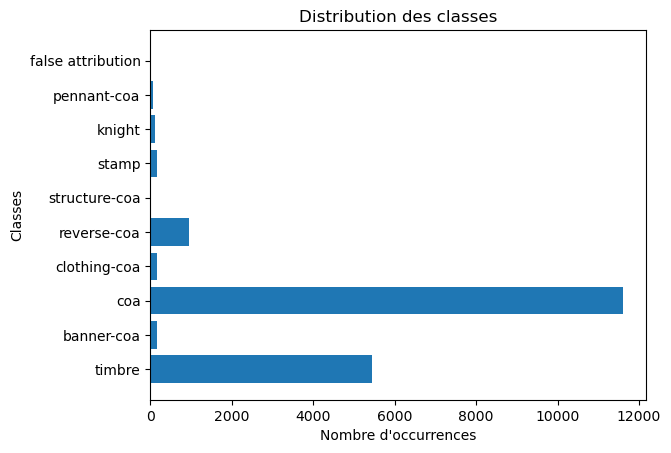
\includegraphics[width=\textwidth]{class_distributiontrain_group_7_20230915_l_i640_e100_b8_w24.png}
    \end{minipage}
    \hfill
    \begin{minipage}[b]{0.45\textwidth}
        \centering
        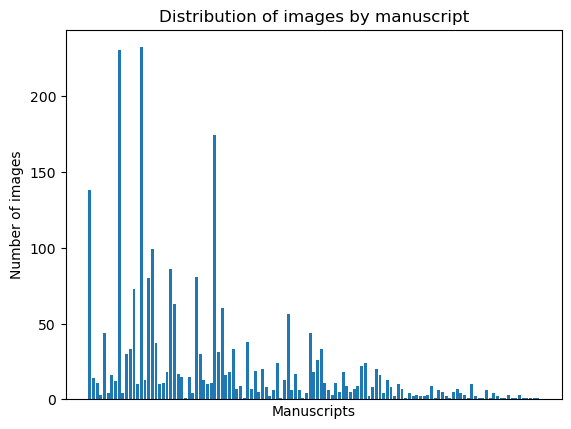
\includegraphics[width=\textwidth]{img_per_ms_train_group_7_20230915_l_i640_e100_b8_w24.png}
    \end{minipage}
\end{figure}

\begin{center}
\begin{table}[ht]
    \centering
    \caption{Données globales du modèle \textit{Coat of Arms}}
    \begin{tabular}{|c|c|}
    \hline
    \textbf{Métrique} & \textbf{Valeur} \\
    \hline
    Nombre de manuscrits & 123 \\ 
    \hline
    Nombre d'images sans annotations & 94 \\ 
    \hline
    Nombre total d'annotations & 18688 \\ 
    \hline
    \end{tabular}
\end{table}    
\end{center}


\newpage
\subsection{\textit{Coat of Arms non shield coa}}

\begin{verbatim}
Nom du modèle : Grouped_non_shield_coa_20230915_l_i640_e100_b8_w24
Algorithme : YOLOv8
Nombre d'époques : 100
Taille du batch : 8
Taille images: 640
Workers : 24
\end{verbatim}


\begin{figure}[ht]
    \centering
    \begin{minipage}[b]{0.45\textwidth}
        \centering
        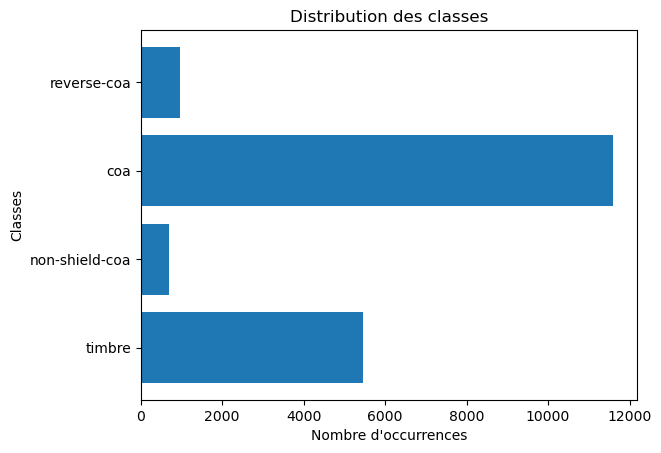
\includegraphics[width=\textwidth]{class_distribution_Grouped_non_shield_coa_20230915_l_i640_e100_b8_w24.png}
    \end{minipage}
    \hfill
    \begin{minipage}[b]{0.45\textwidth}
        \centering
        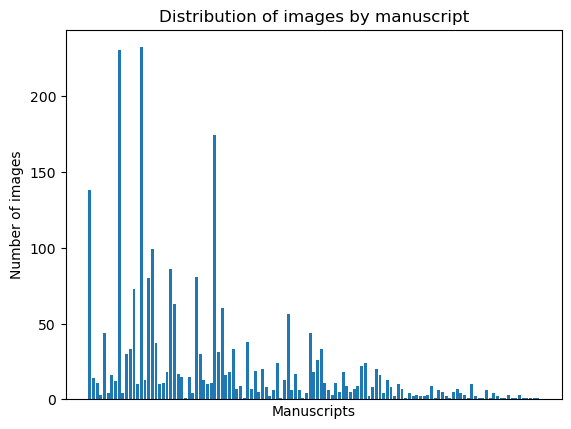
\includegraphics[width=\textwidth]{img_per_ms_Grouped_non_shield_coa_20230915_l_i640_e100_b8_w24.png}
    \end{minipage}
\end{figure}

\begin{center}
\begin{table}[ht]
    \centering
    \caption{Données globales du modèle \textit{Coat of Arms non shield coa}}
    \begin{tabular}{|c|c|}
    \hline
    \textbf{Métrique} & \textbf{Valeur} \\
    \hline
    Nombre de manuscrits & 123 \\ 
    \hline
    Nombre d'images sans annotations & 94 \\ 
    \hline
    Nombre total d'annotations & 18688 \\ 
    \hline
    \end{tabular}
\end{table}    
\end{center}

\newpage
\subsection{\textit{Coat of Arms Isodata}}

\begin{verbatim}
Nom du modèle : COA_Isodata_20230918_l_i640_e100_b8_w24
Algorithme : YOLOv8
Nombre d'époques : 100
Taille du batch : 8
Taille images: 640
Workers : 24
\end{verbatim}


\begin{figure}[ht]
    \centering
    \begin{minipage}[b]{0.45\textwidth}
        \centering
        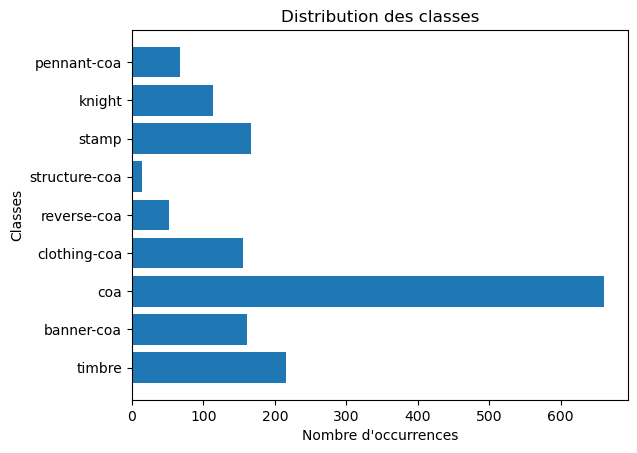
\includegraphics[width=\textwidth]{class_distribution_COA_Isodata_20230918_l_i640_e100_b8_w24.png}
    \end{minipage}
    \hfill
    \begin{minipage}[b]{0.45\textwidth}
        \centering
        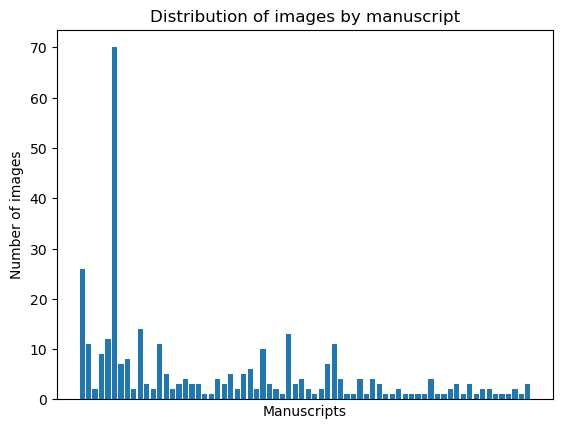
\includegraphics[width=\textwidth]{img_per_ms_COA_Isodata_20230918_l_i640_e100_b8_w24.png}
    \end{minipage}
\end{figure}

\begin{center}
\begin{table}[ht]
    \centering
    \caption{Données globales du modèle \textit{Coat of Arms Isodata}}
    \begin{tabular}{|c|c|}
    \hline
    \textbf{Métrique} & \textbf{Valeur} \\
    \hline
    Nombre de manuscrits & 70 \\ 
    \hline
    Nombre d'images sans annotations & 0 \\ 
    \hline
    Nombre total d'annotations & 1607 \\ 
    \hline
    \end{tabular}
\end{table}    
\end{center}


\newpage
\subsection{\textit{Coat of Arms shapes}}

\begin{verbatim}
Nom du modèle : COA_shapes_20230916_l_i640_e100_b8_w24
Algorithme : YOLOv8
Nombre d'époques : 100
Taille du batch : 8
Taille images: 640
Workers : 24
\end{verbatim}


\begin{figure}[ht]
    \centering
    \begin{minipage}[b]{0.45\textwidth}
        \centering
        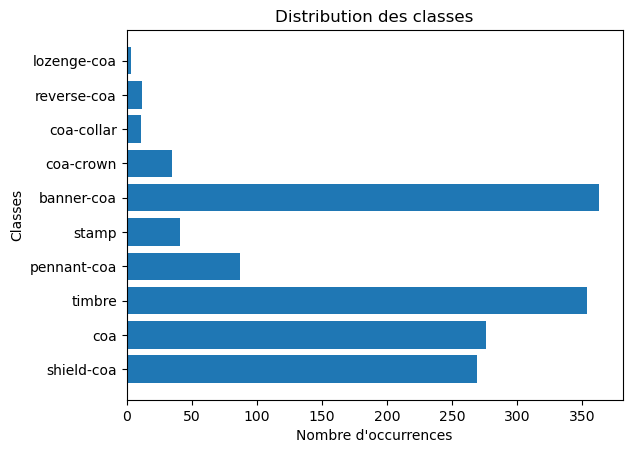
\includegraphics[width=\textwidth]{class_distribution_COA_shapes_20230916_l_i640_e100_b8_w24.png}
    \end{minipage}
    \hfill
    \begin{minipage}[b]{0.45\textwidth}
        \centering
        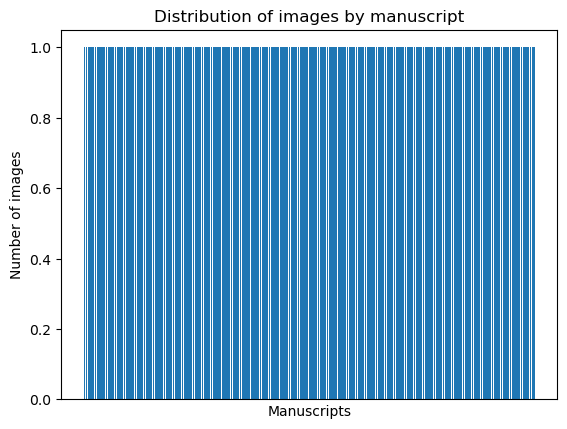
\includegraphics[width=\textwidth]{img_per_ms_COA_shapes_20230916_l_i640_e100_b8_w24.png}
    \end{minipage}
\end{figure}

\begin{center}
\begin{table}[ht]
    \centering
    \caption{Données globales du modèle \textit{Coat of Arms shapes}}
    \begin{tabular}{|c|c|}
    \hline
    \textbf{Métrique} & \textbf{Valeur} \\
    \hline
    Nombre de manuscrits & 249 \\ 
    \hline
    Nombre d'images sans annotations & 3 \\ 
    \hline
    Nombre total d'annotations & 1451 \\ 
    \hline
    \end{tabular}
\end{table}    
\end{center}

\newpage
\section{Miniatures}
\subsection{Miniatures}

\begin{verbatim}
Nom du modèle : Miniatures_20230915_l_i640_e100_b8_w24
Algorithme : YOLOv8
Nombre d'époques : 100
Taille du batch : 8
Taille images: 640
Workers : 24
\end{verbatim}


\begin{figure}[ht]
    \centering
    \begin{minipage}[b]{0.45\textwidth}
        \centering
        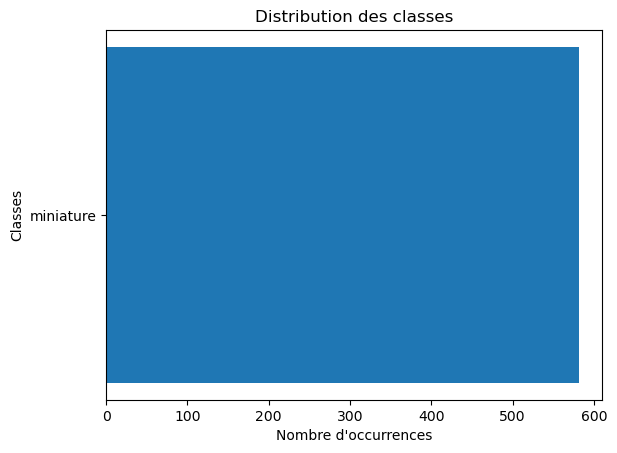
\includegraphics[width=\textwidth]{class_distribution_Miniatures_20230915_l_i640_e100_b8_w24.png}
    \end{minipage}
    \hfill
    \begin{minipage}[b]{0.45\textwidth}
        \centering
        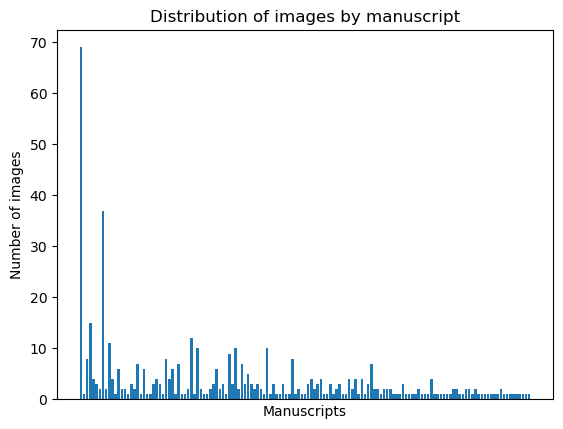
\includegraphics[width=\textwidth]{img_per_ms_Miniatures_20230915_l_i640_e100_b8_w24.png}
    \end{minipage}
\end{figure}

\begin{center}
\begin{table}[ht]
    \centering
    \caption{Données globales du modèle Miniatures}
    \begin{tabular}{|c|c|}
    \hline
    \textbf{Métrique} & \textbf{Valeur} \\
    \hline
    Nombre de manuscrits & 143 \\ 
    \hline
    Nombre d'images sans annotations & 0 \\ 
    \hline
    Nombre total d'annotations & 581 \\ 
    \hline
    \end{tabular}
\end{table}    
\end{center}

\newpage
\subsection{Miniatures \textit{new classes}}

\begin{verbatim}
Nom du modèle : Miniatures_new_classes_20230916_l_i640_e100_b8_w24
Algorithme : YOLOv8
Nombre d'époques : 100
Taille du batch : 8
Taille images: 640
Workers : 24
\end{verbatim}


\begin{figure}[ht]
    \centering
    \begin{minipage}[b]{0.45\textwidth}
        \centering
        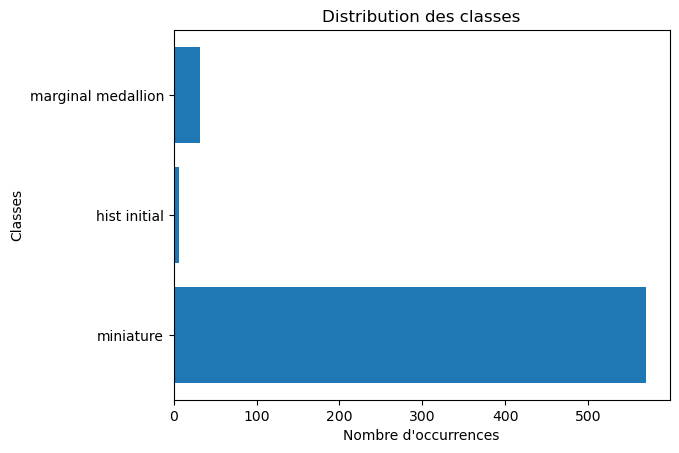
\includegraphics[width=\textwidth]{class_distribution_Miniatures_new_classes_20230916_l_i640_e100_b8_w24.png}
    \end{minipage}
    \hfill
    \begin{minipage}[b]{0.45\textwidth}
        \centering
        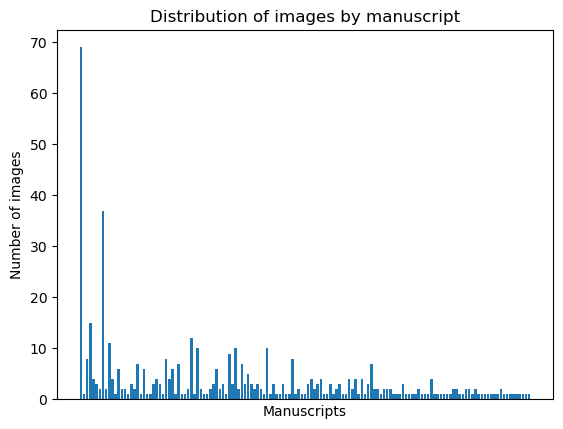
\includegraphics[width=\textwidth]{img_per_ms_Miniatures_new_classes_20230916_l_i640_e100_b8_w24.png}
    \end{minipage}
\end{figure}

\begin{center}
\begin{table}[ht]
    \centering
    \caption{Données globales du modèle Miniatures \textit{new classes}}
    \begin{tabular}{|c|c|}
    \hline
    \textbf{Métrique} & \textbf{Valeur} \\
    \hline
    Nombre de manuscrits & 143 \\ 
    \hline
    Nombre d'images sans annotations & 0 \\ 
    \hline
    Nombre total d'annotations & 609 \\ 
    \hline
    \end{tabular}
\end{table}    
\end{center}

\newpage
\section{\textit{Books in books}}
\subsection{\textit{Books in books}}

\begin{verbatim}
Nom du modèle : Books_in_books_20230910_l_i640_e100_b8_w24
Algorithme : YOLOv8
Nombre d'époques : 100
Taille du batch : 8
Taille images: 640
Workers : 24
\end{verbatim}


\begin{figure}[ht]
    \centering
    \begin{minipage}[b]{0.45\textwidth}
        \centering
        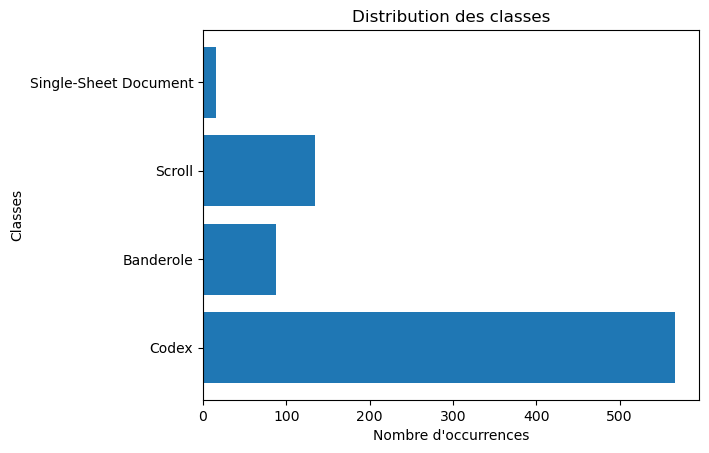
\includegraphics[width=\textwidth]{class_distribution_Books_in_books_20230910_l_i640_e100_b8_w24.png}
    \end{minipage}
    \hfill
    \begin{minipage}[b]{0.45\textwidth}
        \centering
        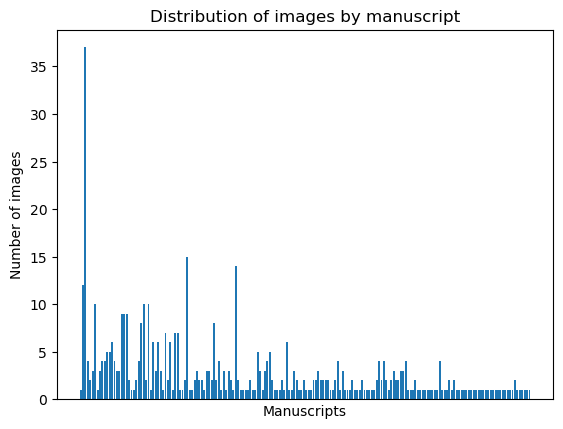
\includegraphics[width=\textwidth]{img_per_ms_Books_in_books_20230910_l_i640_e100_b8_w24.png}
    \end{minipage}
\end{figure}

\begin{center}
\begin{table}[ht]
    \centering
    \caption{Données globales du modèle \textit{Books in books}}
    \begin{tabular}{|c|c|}
    \hline
    \textbf{Métrique} & \textbf{Valeur} \\
    \hline
    Nombre de manuscrits & 186 \\ 
    \hline
    Nombre d'images sans annotations & 0 \\ 
    \hline
    Nombre total d'annotations & 805 \\ 
    \hline
    \end{tabular}
\end{table}    
\end{center}

\newpage
\subsection{\textit{Books in books new data}}

\begin{verbatim}
Nom du modèle : Books_in_books_new_data_20230916_l_i640_e100_b8_w24
Algorithme : YOLOv8
Nombre d'époques : 100
Taille du batch : 8
Taille images: 640
Workers : 24
\end{verbatim}


\begin{figure}[ht]
    \centering
    \begin{minipage}[b]{0.45\textwidth}
        \centering
        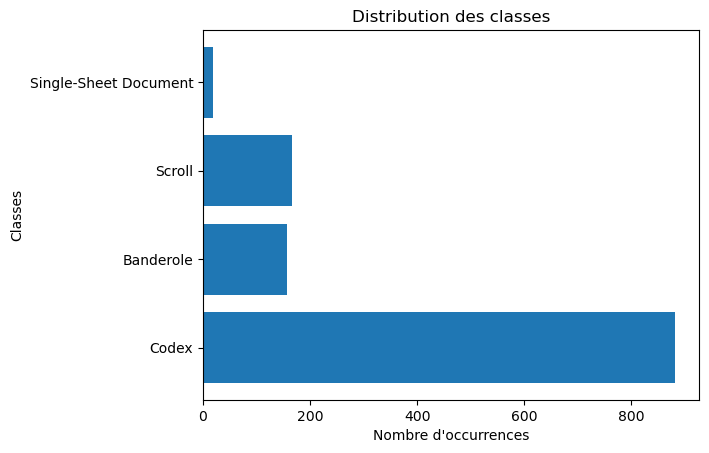
\includegraphics[width=\textwidth]{class_distribution_Books_in_books_new_data_20230916_l_i640_e100_b8_w24.png}
    \end{minipage}
    \hfill
    \begin{minipage}[b]{0.45\textwidth}
        \centering
        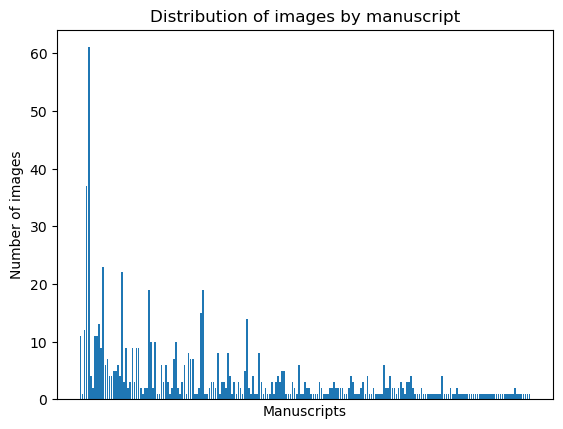
\includegraphics[width=\textwidth]{img_per_ms_Books_in_books_new_data_20230916_l_i640_e100_b8_w24.png}
    \end{minipage}
\end{figure}

\begin{center}
\begin{table}[ht]
    \centering
    \caption{Données globales du modèle \textit{Books in books new data}}
    \begin{tabular}{|c|c|}
    \hline
    \textbf{Métrique} & \textbf{Valeur} \\
    \hline
    Nombre de manuscrits & 217 \\ 
    \hline
    Nombre d'images sans annotations & 0 \\ 
    \hline
    Nombre total d'annotations & 1224 \\ 
    \hline
    \end{tabular}
\end{table}    
\end{center}



\backmatter

\printindex
\cleardoublepage
\phantomsection
\addcontentsline{toc}{chapter}{Liste des figures}
\listoffigures


\cleardoublepage
\phantomsection
\addcontentsline{toc}{chapter}{Liste des tableaux}
\listoftables

\tableofcontents




\end{document}
